\documentclass[9pt,a5paper,]{book}
\usepackage{lmodern}
\usepackage{amssymb,amsmath}
\usepackage{ifxetex,ifluatex}
\usepackage{fixltx2e} % provides \textsubscript
\ifnum 0\ifxetex 1\fi\ifluatex 1\fi=0 % if pdftex
  \usepackage[T1]{fontenc}
  \usepackage[utf8]{inputenc}
\else % if luatex or xelatex
  \ifxetex
    \usepackage{mathspec}
  \else
    \usepackage{fontspec}
  \fi
  \defaultfontfeatures{Ligatures=TeX,Scale=MatchLowercase}
\fi
% use upquote if available, for straight quotes in verbatim environments
\IfFileExists{upquote.sty}{\usepackage{upquote}}{}
% use microtype if available
\IfFileExists{microtype.sty}{%
\usepackage{microtype}
\UseMicrotypeSet[protrusion]{basicmath} % disable protrusion for tt fonts
}{}
\usepackage[left=2cm,right=1.2cm,top=1.5cm,bottom=1.5cm]{geometry}
\usepackage{hyperref}
\hypersetup{unicode=true,
            pdftitle={Regression Models for Count Data: beyond the Poisson model},
            pdfauthor={Wagner Hugo Bonat; Walmes Marques Zeviani; Eduardo Elias Ribeiro Jr},
            pdfborder={0 0 0},
            breaklinks=true}
\urlstyle{same}  % don't use monospace font for urls
\usepackage{natbib}
\bibliographystyle{apalike}
\usepackage{color}
\usepackage{fancyvrb}
\newcommand{\VerbBar}{|}
\newcommand{\VERB}{\Verb[commandchars=\\\{\}]}
\DefineVerbatimEnvironment{Highlighting}{Verbatim}{commandchars=\\\{\}}
% Add ',fontsize=\small' for more characters per line
\newenvironment{Shaded}{}{}
\newcommand{\KeywordTok}[1]{\textbf{{#1}}}
\newcommand{\DataTypeTok}[1]{\underline{{#1}}}
\newcommand{\DecValTok}[1]{{#1}}
\newcommand{\BaseNTok}[1]{{#1}}
\newcommand{\FloatTok}[1]{{#1}}
\newcommand{\ConstantTok}[1]{{#1}}
\newcommand{\CharTok}[1]{{#1}}
\newcommand{\SpecialCharTok}[1]{{#1}}
\newcommand{\StringTok}[1]{{#1}}
\newcommand{\VerbatimStringTok}[1]{{#1}}
\newcommand{\SpecialStringTok}[1]{{#1}}
\newcommand{\ImportTok}[1]{{#1}}
\newcommand{\CommentTok}[1]{\textit{{#1}}}
\newcommand{\DocumentationTok}[1]{\textit{{#1}}}
\newcommand{\AnnotationTok}[1]{\textit{{#1}}}
\newcommand{\CommentVarTok}[1]{\textit{{#1}}}
\newcommand{\OtherTok}[1]{{#1}}
\newcommand{\FunctionTok}[1]{{#1}}
\newcommand{\VariableTok}[1]{{#1}}
\newcommand{\ControlFlowTok}[1]{\textbf{{#1}}}
\newcommand{\OperatorTok}[1]{{#1}}
\newcommand{\BuiltInTok}[1]{{#1}}
\newcommand{\ExtensionTok}[1]{{#1}}
\newcommand{\PreprocessorTok}[1]{\textbf{{#1}}}
\newcommand{\AttributeTok}[1]{{#1}}
\newcommand{\RegionMarkerTok}[1]{{#1}}
\newcommand{\InformationTok}[1]{\textit{{#1}}}
\newcommand{\WarningTok}[1]{\textit{{#1}}}
\newcommand{\AlertTok}[1]{\textbf{{#1}}}
\newcommand{\ErrorTok}[1]{\textbf{{#1}}}
\newcommand{\NormalTok}[1]{{#1}}
\usepackage{longtable,booktabs}
\usepackage{graphicx,grffile}
\makeatletter
\def\maxwidth{\ifdim\Gin@nat@width>\linewidth\linewidth\else\Gin@nat@width\fi}
\def\maxheight{\ifdim\Gin@nat@height>\textheight\textheight\else\Gin@nat@height\fi}
\makeatother
% Scale images if necessary, so that they will not overflow the page
% margins by default, and it is still possible to overwrite the defaults
% using explicit options in \includegraphics[width, height, ...]{}
\setkeys{Gin}{width=\maxwidth,height=\maxheight,keepaspectratio}
\IfFileExists{parskip.sty}{%
\usepackage{parskip}
}{% else
\setlength{\parindent}{0pt}
\setlength{\parskip}{6pt plus 2pt minus 1pt}
}
\setlength{\emergencystretch}{3em}  % prevent overfull lines
\providecommand{\tightlist}{%
  \setlength{\itemsep}{0pt}\setlength{\parskip}{0pt}}
\setcounter{secnumdepth}{5}
% Redefines (sub)paragraphs to behave more like sections
\ifx\paragraph\undefined\else
\let\oldparagraph\paragraph
\renewcommand{\paragraph}[1]{\oldparagraph{#1}\mbox{}}
\fi
\ifx\subparagraph\undefined\else
\let\oldsubparagraph\subparagraph
\renewcommand{\subparagraph}[1]{\oldsubparagraph{#1}\mbox{}}
\fi

%%% Use protect on footnotes to avoid problems with footnotes in titles
\let\rmarkdownfootnote\footnote%
\def\footnote{\protect\rmarkdownfootnote}

%%% Change title format to be more compact
\usepackage{titling}

% Create subtitle command for use in maketitle
\newcommand{\subtitle}[1]{
  \posttitle{
    \begin{center}\large#1\end{center}
    }
}

\setlength{\droptitle}{-2em}
  \title{Regression Models for Count Data: beyond the Poisson model}
  \pretitle{\vspace{\droptitle}\centering\huge}
  \posttitle{\par}
  \author{Wagner Hugo Bonat \\ Walmes Marques Zeviani \\ Eduardo Elias Ribeiro Jr}
  \preauthor{\centering\large\emph}
  \postauthor{\par}
  \date{}
  \predate{}\postdate{}

% Mathematics environments
\usepackage{amssymb}
\usepackage{amsmath}
\usepackage{amstext}
\usepackage{amsfonts}

% Figures
\usepackage{graphics}
\usepackage{natbib}

% Customize itemize's enviroments
\usepackage{enumitem}

% Fonts
\usepackage{mathpazo}
\usepackage{eulervm}
\usepackage{inconsolata}
\urlstyle{tt}

% Compact toc
\usepackage{tocloft}

% Footers and headers styles
\usepackage{fancyhdr}
\pagestyle{fancy}
\fancyhf{}
\fancyhead[LE,RO]{\thepage}
\fancyhead[RE]{\scriptsize\leftmark}
\fancyhead[LO]{\scriptsize\rightmark}

% Modify color in Rcodes/chunks (works well only monochrome highlight)
\usepackage{xcolor}
\definecolor{inputcolor}{RGB}{25,25,112}
\usepackage{framed}
\usepackage{fancyvrb}
\DefineVerbatimEnvironment{Highlighting}{Verbatim}{commandchars=\\\{\},
                                                   fontsize=\small}
\definecolor{shadecolor}{RGB}{248,248,248}
\renewenvironment{Shaded}{\color{inputcolor}}{}
\renewcommand{\DataTypeTok}[1]{{#1}}

% Modify style of verbatim (chunks outputs)
\definecolor{outputcolor}{RGB}{139,0,0}
\makeatletter
\def\verbatim@font{\ttfamily \small \color{outputcolor}}%
\makeatother

% % For table placemente (knitr::kable don't provides this option)
% \usepackage{float}
% \makeatletter
% \renewcommand{\fps@table}{H}
% \makeatother

\usepackage{amsthm}
\newtheorem{theorem}{Theorem}[chapter]
\newtheorem{lemma}{Lemma}[chapter]
\theoremstyle{definition}
\newtheorem{definition}{Definition}[chapter]
\newtheorem{corollary}{Corollary}[chapter]
\newtheorem{proposition}{Proposition}[chapter]
\theoremstyle{definition}
\newtheorem{example}{Example}[chapter]
\theoremstyle{remark}
\newtheorem*{remark}{Remark}
\begin{document}
\maketitle

\thispagestyle{empty}
\cleardoublepage
\thispagestyle{empty}

\topskip0pt

\begin{flushleft}
  \Large \bf
  Regression Models for Count Data:\\
  beyond Poisson model
\end{flushleft}
\vspace*{1.5em}

\begin{flushleft}
Wagner Hugo Bonat\footnotemark[1] \footnotemark[3]\\
\url{www.leg.ufpr.br/~wagner}

Walmes Marques Zeviani\footnotemark[1] \footnotemark[3]\\
\url{www.leg.ufpr.br/~walmes}

Eduardo Elias Ribeiro Jr\footnotemark[2] \footnotemark[3]\\
\url{www.leg.ufpr.br/~eduardojr}
\end{flushleft}
\vspace*{2em}


\footnotemark[1]Departamento de Estatística (DEST)\\
\hspace*{1.5mm}Universidade Federal do Paraná (UFPR)

\footnotemark[2]Departamento de Ciências Exatas (LCE)\\
\hspace*{1.5mm}ESALQ - Universidade de São Paulo (ESALQ-USP)

\footnotemark[3]Laboratório de Estatística e Geoinformação (LEG)\\
\hspace*{1.5mm}\url{http://www.leg.ufpr.br}\\

Supplementary content: \url{http://www.leg.ufpr.br/rmcd}\\
Contact: \url{rmcd@leg.ufpr.br}
\vspace*{\fill}

\begin{center}
XV EMR - Escola de Modelos de Regressão\\
Goiânia - Goiás, Brasil\\
March 26 to 29, 2017
\end{center}

\clearpage
\thispagestyle{empty}
\pagebreak

\setcounter{page}{1}

{
\setcounter{tocdepth}{1}
\tableofcontents
}
\chapter*{Preface}\label{preface}
\addcontentsline{toc}{chapter}{Preface}

The main goal of this material is to provide a technical support for the
students attending the course ''Regression models for count data: beyond
the Poisson model``, given as part of the XV Brazilian School of
Regression models - March/2017 in Goiânia, Goiás, Brazil.

The main goal of this course is to present a wide range of statistical
models to deal with count data. We focus on parametric and second-moment
specified models. We shall present the model specification along with
strategies for model fitting and associated \texttt{R}\citep{R2015}
code. Furthermore, this book-course and supplementary materials, such as
\texttt{R} code and data sets are available for the students on the web
page \url{http://cursos.leg.ufpr.br/rmcd}.

We intend to keep the course in a level suitable for bachelor students
who already attended a course on generalized linear models
\citep{Nelder1972}. However, since the course also covers updated
topics, it can be of interest of postgraduate students and researches in
general.

We designed the course for three hours of tuition. In the first part of
the course, we shall present the analysis of count data based on fully
parametric models. After a brief introduction and motivation on count
data, we present the Poisson, Gamma-Count, Poisson-Tweedie and
COM-Poisson distributions. We explore their properties through a
consideration of dispersion, zero-inflated and heavy tail indexes.
Furthermore, the estimation and inference for these models based on the
likelihood paradigm is discussed along with the associated \texttt{R}
code and worked examples.

In the second part of the course, we provide a brief introduction to the
estimating function approach \citetext{\citealp[
]{Jorgensen2004}; \citealp{Bonat2016a}} and discuss models based on
second-moment assumptions in the style of \citet{Wedderburn1974}. In
particular, we focus on the recently proposed Extended Poisson-Tweedie
model \citep{Bonat2016b} and its special case the quasi-Poisson model.
The estimating function approach adopted for estimation and inference is
presented along with \texttt{R} code and data examples. The use of the
\texttt{R} package \texttt{mcglm} \citep{Bonat2016c} is discussed for
fitting the extended Poisson-Tweedie model.

We acknowledge our gratitude to the scientific committee of XV Brazilian
regression model school for this opportunity.

Department of Statistics, Paraná Federal University, Curitiba, PR,
Brazil.

March 27, 2017.

\chapter{Introduction}\label{introduction}

The analysis of count data has received attention from the statistical
community in the last four decades. Since the seminal paper published by
\citet{Nelder1972}, the class of generalized linear models (GLMs) have a
prominent role for regression modelling of normal and non-normal data.
GLMs are fitted by a simple and efficient Newton scoring algorithm
relying only on second-moment assumptions for estimation and inference.
Furthermore, the theoretical background for GLMs is well established in
the class of dispersion models \citep{Jorgensen1987, Jorgensen1997} as a
generalization of the exponential family of distributions.

In spite of the flexibility of the GLM class, the Poisson distribution
is the only choice for the analysis of count data in this framework.
Thus, in practice there is probably an over-emphasis on the use of the
Poisson distribution for count data. A well known limitation of the
Poisson distribution is its mean and variance relationship, which
implies that the variance equals the mean, referred to as
equidispersion. In practice, however, count data can present other
features, namely underdispersion (mean \textgreater{} variance) and
overdispersion (mean \textless{} variance). There are many different
possible causes for departures from the equidispersion. Furthermore, in
practical data analysis a number of these could be involved.

One possible cause of under/overdispersion is departure from the Poisson
process. It is well known that the Poisson counts can be interpreted as
the number of events in a given time interval where the arrival's times
are exponential distributed. In the cases where this assumption is
violated the resulting counts can be under or overdispersed
\citep{Zeviani2014}. Another possibility and probably more frequent
cause of overdispersion is unobserved heterogeneity of experimental
units. It can be due, for example, to correlation between individual
responses, cluster sampling, omitted covariates and others.

In general, these departures from the Poisson distribution are
manifested in the raw data as a zero-inflated or heavy-tailed count
distribution. It is important to discuss the consequences of failing to
take into account the under or overdispersion when analysing count data.
In the case of overdispersion, the standard errors associated with the
regression coefficients calculated under the Poisson assumption are too
optimistic and associated hypothesis tests will tend to give false
positive results by incorrectly rejecting null hypotheses. The opposite
situation will appear in case of underdispersed data. In both cases, the
Poisson model provides unreliable standard errors for the regression
coefficients and hence potentially misleading inferences. However, the
regression coefficients are still consistently estimated.

The strategies for constructing alternative count distributions are
related with the causes of the non-equidispersion. When departures from
the Poisson process are plausible the class of duration dependence
models \citep{Winkelmann2003} can be employed. This class of models
changes the distribution of the time between events from the exponential
to more general distributions, such as gamma and inverse Gaussian. In
this course, we shall discuss one example of this approach, namely, the
Gamma-Count distribution \citep{Zeviani2014}. This distribution assumes
that the time between events is gamma distributed, thus it can deal with
under, equi and overdispersed count data.

On the other hand, if unobserved heterogeneity is present its in general
implies extra variability and consequently overdispersed count data. In
this case, a Poisson mixtures is commonly applied. This approach
consists of include random effects on the observation level, and thus
take into account the unobserved heterogeneity. Probably, the most
popular example of this approach is the negative binomial model, that
corresponds to a Poisson-gamma mixtures. In this course, we shall
present the Poisson-Tweedie family of distributions, which in turn
corresponds to Poisson-Tweedie mixtures
\citep{Bonat2016b, Jorgensen2014}. Finally, a third approach to deal
with non-equidispersed count data consists of generalize the Poisson
distribution by adding an extra parameter to model under and
overdispersion. Such a generalization can be done using the class of
weighted Poisson distributions \citep{DelCastillo1998}. One popular
example of this approach is the Conway--Maxwell--Poisson distribution
(COM-Poisson) \citep{Sellers2010}. The COM-Poisson is a member of the
exponential family, has the Poisson and geometric distributions as
special cases and the Bernoulli distribution as a limiting case. It can
deal with both under and overdispersed count data. Thus, given the nice
properties of the COM-Poisson distribution for handling count data, we
chose to present this model as part of this course.

In this course, we shall highlight and compare the flexibility of these
distributions to deal with count data through a consideration of
dispersion, zero-inflated and heavy tail indexes. Furthermore, we
specify regression models and illustrate their application with three
worked examples.

In Chapter \ref{models} we present the properties and regression models
associated with the Poisson, Gamma-count, Poisson-Tweedie and
COM-Poisson distributions. Furthermore, we compare these distributions
using the dispersion, zero-inflated and heavy tail indexes. Estimation
and inference for these models based on the likelihood paradigm are
discussed in Chapter \ref{likelihood}. In Chapter \ref{SM}, we extend
the Poisson-Tweedie model using only second-moment assumptions and
present the fitting algorithm based on the estimating functions
approach. Chapter \(5\) presents three worked examples.

\chapter{Count distributions: properties and regression
models}\label{models}

In this chapter, we present the probability mass function and discuss
the main properties of the Poisson, Gamma-Count, Poisson-Tweedie and
COM-Poisson distributions.

\section{Poisson distribution}\label{poisson-distribution}

The Poisson distribution is a notorious discrete distribution. It has a
dual interpretation as a natural exponential family and as an
exponential dispersion model. The Poisson distribution denoted by
\(P(\mu)\) has probability mass function

\begin{eqnarray}
p(y;\mu) &=& \frac{\mu^y}{y!}\exp\{-\mu\} \nonumber \\
         &=& \frac{1}{y!} \exp \{\phi y -  \exp\{\phi\} \}, \quad y \in \mathbb{N}_{0},
\label{eq:Poisson}
\end{eqnarray}

where \(\phi = \log \{\mu\} \in \mathbb{R}\). Hence the Poisson is a
natural exponential family with cumulant generator
\(\kappa(\phi) = \exp\{\phi\}\). We have
\(\mathrm{E}(Y) = \kappa^{\prime}(\phi) = \exp\{\phi\} = \mu\) and
\(\mathrm{var}(Y) = \kappa^{\prime \prime}(\phi) = \exp\{\phi\} = \mu\).
The probability mass function \eqref{eq:Poisson} can be evaluated in
\texttt{R} through the \texttt{dpois()} function.

In order to specify a regression model based on the Poisson
distribution, we consider a cross-section dataset, \((y_i, x_i)\),
\(i = 1,\ldots, n\), where \(y_i\)'s are iid realizations of \(Y_i\)
according to a Poisson distribution. The Poisson regression models is
defined by
\[Y_i \sim P(\mu_i), \quad  \text{with} \quad \mu_i = g^{-1}(\boldsymbol{x_i}^{\top} \boldsymbol{\beta}).\]
In this notation, \(\boldsymbol{x_i}\) and \(\boldsymbol{\beta}\) are
(\(p \times 1\)) vectors of known covariates and unknown regression
parameters, respectively. Moreover, \(g\) is a standard link function,
for which we adopt the logarithm link function, but potentially any
other suitable link function could be adopted.

\section{Gamma-Count distribution}\label{gammacount}

The Poisson distribution as presented in \eqref{eq:Poisson} follows
directly from the natural exponential family and thus fits in the
generalized linear models (GLMs) framework. Alternatively, the Poisson
distribution can be derived by assuming independent and exponentially
distributed times between events \citep{Zeviani2014}. This derivation
allows for a flexible framework to specify more general models to deal
with under and overdispersed count data.

As point out by \citet{Winkelmann2003} the distributions of the arrival
times determine the distribution of the number of events. Following
\citet{Winkelman1995}, let \({\tau_k, k \in \mathbb{N}}\) denote a
sequence of waiting times between the \((k-1)\)th and the \(k\)th
events. Then, the arrival time of the \(y\)th event is given by
\(\nu_y = \sum_{k = 1}^{y} \tau_k\), for \(y = 1, 2, \ldots\).
Furthermore, denote \(Y\) the total number of events in the open
interval between \(0\) and \(T\). For fixed \(T\), \(Y\) is a count
variable. Indeed, from the definitions of \(Y\) and \(\nu_y\) we have
that \(Y < y\) iff \(\nu_y \ge T\), which in turn implies
\(P(Y < y) = P(\nu_y \ge T) = 1 - F_y(T)\), where \(F_y(T)\) denotes the
cumulative distribution function of \(\nu_y\). Furthermore,

\begin{eqnarray}
P(Y = y) &=& P(Y < y+1) - P(Y < y) \nonumber \\
     &=& F_y(T) - F_{y+1}(T).
\label{eq:DURATION}
\end{eqnarray}

Equation \eqref{eq:DURATION} provides the fundamental relation between the
distribution of arrival times and the distribution of counts. Moreover,
this type of specification allows to derive a rich class of models for
count data by choosing a distribution for the arrival times. In this
material, we shall explore the Gamma-Count distribution which is
obtained by specifying the arrival times distribution as gamma
distributed.

Let \(\tau_k\) be identically and independently gamma distributed, with
density distribution (dropping the index \(k\)) given by

\begin{equation}
f(\tau; \alpha, \gamma) = \frac{\gamma^{\alpha}}{\Gamma(\alpha)} \tau^{\alpha-1} \exp\{-\gamma \tau\}, \quad \alpha, \gamma \in \mathbb{R}^{+}.
\end{equation}

In this parametrization \(\mathrm{E}(\tau) = \alpha/\gamma\) and
\(\mathrm{var}(\tau) = \alpha/\gamma^2\). Thus, by applying the
convolution formula for gamma distributions, it is easy to show that the
distribution of \(\nu_y\) is given by

\begin{equation}
f_y(\nu; \alpha, \gamma) = \frac{\gamma^{y\alpha}}{\Gamma(y\alpha)} \nu^{y\alpha-1} \exp\{-\gamma \nu\}.
\end{equation}

To derive the new count distribution, we have to evaluate the cumulative
distribution function, which after the change of variable
\(u = \gamma \alpha\) can be written as

\begin{equation}
F_y(T) = \frac{1}{\Gamma(y\alpha)} \int_0^{\gamma T} u^{n\alpha -1} \exp\{-u\} du,
\label{eq:INTEGRAL}
\end{equation}

where the integral is the incomplete gamma function. We denote the right
side of \eqref{eq:INTEGRAL} as \(G(\alpha y, \gamma T)\). Thus, the number
of event occurrences during the time interval \((0,T)\) has the
two-parameter distribution function

\begin{equation}
P(Y = y) = G(\alpha y, \gamma T) - G(\alpha (y + 1), \gamma T),
\label{eq:MASSFUNCTION}
\end{equation}

for \(y = 0, 1, \ldots\), where \(\alpha, \gamma \in \mathbb{R}^+\).
\citet{Winkelman1995} showed that for integer \(\alpha\) the probability
mass function defined in \eqref{eq:MASSFUNCTION} is given by

\begin{equation}
P(Y = y) = \exp^{\{-\gamma T\}} \sum_{i = 0}^{\alpha -1} \frac{(\gamma T)^{\alpha y + i}}{\alpha y + i}!.
\end{equation}

For \(\alpha = 1\), \(f(\tau)\) is the exponential distribution and
\eqref{eq:MASSFUNCTION} clearly simplifies to the Poisson distribution.
The following \texttt{R} function can be used to evaluate the
probability mass function of the Gamma-Count distribution.

\begin{Shaded}
\begin{Highlighting}[]
\NormalTok{dgc <-}\StringTok{ }\NormalTok{function(y, gamma, alpha, }\DataTypeTok{log =} \OtherTok{FALSE}\NormalTok{) \{}
  \NormalTok{p <-}\StringTok{ }\KeywordTok{pgamma}\NormalTok{(}\DataTypeTok{q =} \DecValTok{1}\NormalTok{,}
              \DataTypeTok{shape =} \NormalTok{y *}\StringTok{ }\NormalTok{alpha,}
              \DataTypeTok{rate =} \NormalTok{alpha *}\StringTok{ }\NormalTok{gamma) -}
\StringTok{    }\KeywordTok{pgamma}\NormalTok{(}\DataTypeTok{q =} \DecValTok{1}\NormalTok{,}
           \DataTypeTok{shape =} \NormalTok{(y +}\StringTok{ }\DecValTok{1}\NormalTok{) *}\StringTok{ }\NormalTok{alpha,}
           \DataTypeTok{rate =} \NormalTok{alpha *}\StringTok{ }\NormalTok{gamma)}
  \NormalTok{if(log ==}\StringTok{ }\OtherTok{TRUE}\NormalTok{) \{p <-}\StringTok{ }\KeywordTok{log}\NormalTok{(p)\}}
  \KeywordTok{return}\NormalTok{(p)}
\NormalTok{\}}
\end{Highlighting}
\end{Shaded}

Although, numerical evaluation of \eqref{eq:MASSFUNCTION} can easily be
done, the moments (mean and variance) cannot be obtained in closed form.
\citet{Winkelman1995} showed for a random variable
\(Y \sim GC(\alpha, \gamma)\), where \(GC(\alpha, \gamma)\) denotes a
Gamma-Count distribution with parameters \(\alpha\) and \(\gamma\),
\(\mathrm{E}(Y) = \sum_{i = 1}^\infty G(\alpha i, \gamma T)\).

Furthermore, for increasing \(T\) it holds that

\begin{equation}
Y(T) \overset{a}{\sim} N\left(\frac{\gamma T}{\alpha}, \frac{\gamma T}{\alpha^2} \right),
\end{equation}

thus the limiting variance-mean ratio equals a constant \(1/\alpha\).
Consequently, the Gamma-Count distribution displays overdispersion for
\(0 < \alpha < 1\) and underdispersion for \(\alpha > 1\). Figure
\ref{fig:PlotGC} presents the probability mass function for some
Gamma-Count distributions. We fixed the parameter \(\gamma = 10\) and
fit the parameter \(\alpha\) in order to have dispersion index
(\(\mathrm{DI} = \mathrm{var}(Y)/\mathrm{E}(Y)\)) equalling to \(0.5\),
\(2\), \(5\) and \(20\).

\begin{figure}[h]

{\centering 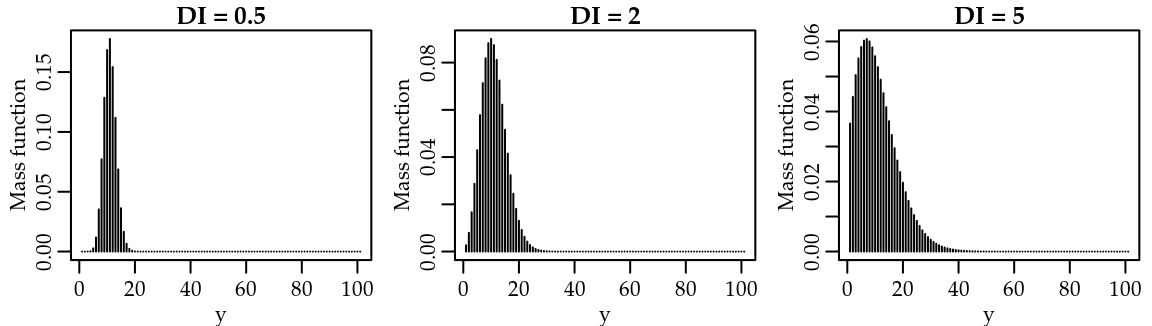
\includegraphics{rmcdbook_files/figure-latex/PlotGC-1} 

}

\caption{Gamma-Count probability mass function by values of the dispersion index (DI).}\label{fig:PlotGC}
\end{figure}

The Gamma-Count regression model assumes that the period at risk \((T)\)
is identical for all observations, thus \(T\) may be set to unity
without loss of generality. In the Gamma-count regression model, the
parameters depend on a vector of individual covariates
\(\boldsymbol{x}_i\). Thus, the Gamma-Count regression model is defined
by

\begin{equation}
\mathrm{E}(\tau_i | \boldsymbol{x}_i) = \frac{\alpha}{\gamma} = g^{-1}(-\boldsymbol{x_i}^\top \boldsymbol{\beta}).
\end{equation}

Consequently, the regression model is for the waiting times and not
directly for the counts. Note that,
\(\mathrm{E}(N_i | \boldsymbol{x}_i) = \mathrm{E}(\tau_i | \boldsymbol{x}_i)^{-1}\)
iff \(\alpha = 1\). Thus, \(\hat{\boldsymbol{\beta}}\) should be
interpreted accordingly. \(-\beta\) measures the percentage change in
the expected waiting time caused by a unit increase in \(x_i\). The
model parameters can be estimated using the maximum likelihood method as
we shall discuss in Chapter \ref{likelihood}.

\section{Poisson-Tweedie distribution}\label{ptw}

The Poisson-Tweedie distribution
\citep{Bonat2016b, Jorgensen2014, Shaarawi2011} consists of include
Tweedie distributed random effects on the observation level of Poisson
random variables, and thus to take into account unobserved
heterogeneity. The Poisson-Tweedie family is given by the following
hierarchical specification

\begin{eqnarray}
Y|Z &\sim& \mathrm{Poisson}(Z) \\
Z &\sim& \mathrm{Tw}_p(\mu, \phi), \nonumber
\label{eq:conditional}
\end{eqnarray}

where \(\mathrm{Tw}_p(\mu, \phi)\) denotes a Tweedie distribution
\citetext{\citealp[ ]{Jorgensen1987}; \citealp{Jorgensen1997}} with
probability function given by

\begin{equation}
f_{Z}(z; \mu, \phi, p) = a(z,\phi,p) \exp\{(z\psi - k_p(\psi))/\phi\}.
\label{eq:tweedie}
\end{equation}

In this notation, \(\mu = k^{\prime}_p(\psi)\) is the expectation,
\(\phi > 0\) is the dispersion parameter, \(\psi\) is the canonical
parameter and \(k_p(\psi)\) is the cumulant function. Furthermore,
\(\mathrm{var}(Z) = \phi V(\mu)\) where
\(V(\mu) = k^{\prime \prime}_p(\psi)\) is the variance function. Tweedie
densities are characterized by power variance functions of the form
\(V(\mu) = \mu^p\), where \(p \in (-\infty ,0] \cup [1,\infty)\) is an
index determining the distribution. The support of the distribution
depends on the value of the power parameter. For \(p \geq 2\),
\(1 < p < 2\) and \(p = 0\) the support corresponds to the positive,
non-negative and real values, respectively. In these cases
\(\mu \in \Omega\), where \(\Omega\) is the convex support (i.e.~the
interior of the closed convex hull of the corresponding distribution
support). Finally, for \(p < 0\) the support corresponds to the real
values, however the expectation \(\mu\) is positive. Here, we required
\(p \geq 1\), to make \(\mathrm{Tw}_p(\mu, \phi)\) non-negative.

The function \(a(z,\phi, p)\) cannot be written in a closed form apart
of the special cases corresponding to the Gaussian (\(p = 0\)), Poisson
(\(\phi = 1\) and \(p = 1\)), non-central gamma (\(p = 3/2\)), gamma
(\(p = 2\)) and inverse Gaussian (\(p = 3\)) distributions
\citep{Jorgensen1997}. The compound Poisson distribution is obtained
when \(1 < p < 2\). This distribution is suitable to deal with
non-negative data with probability mass at zero and highly right-skewed
\citep{Andersen2016}.

The Poisson-Tweedie is an overdispersed factorial dispersion model
\citep{Jorgensen2014} and its probability mass function for \(p > 1\) is
given by

\begin{equation}
f(y;\mu,\phi,p) = \int_0^\infty \frac{z^y \exp{-z}}{y!} a(z,\phi,p) \exp\{(z\psi - k_p(\psi))/\phi\} dz.
\label{eq:pmfPTW}
\end{equation}

The integral \eqref{eq:pmfPTW} has no closed-form apart of the special
case corresponding to the negative binomial distribution, obtained when
\(p = 2\), i.e.~a Poisson gamma mixture. In the case of \(p=1\), the
integral \eqref{eq:pmfPTW} is replaced by a sum and we have the Neyman
Type A distribution. Further special cases include the compound Poisson
\((1 < p < 2)\), factorial discrete positive stable \((p > 2)\) and
Poisson-inverse Gaussian \((p = 3)\) distributions \citetext{\citealp[
]{Jorgensen2014}; \citealp{Kokonendji2004}}.

In spite of other approaches to compute the probability mass function of
the Poisson-Tweedie distribution are available in the literature
\citetext{\citealp[ ]{Esnaola2013}; \citealp{Barabesi2016}}. In this
material, we opted to compute it by numerical evaluation of the integral
in \eqref{eq:pmfPTW} using the Monte Carlo method as implemented by the
following functions.

\begin{Shaded}
\begin{Highlighting}[]
\CommentTok{# Integrand Poisson X Tweedie distributions}
\NormalTok{integrand <-}\StringTok{ }\NormalTok{function(x, y, mu, phi, power) \{}
    \NormalTok{int =}\StringTok{ }\KeywordTok{dpois}\NormalTok{(y, }\DataTypeTok{lambda =} \NormalTok{x)*}\KeywordTok{dtweedie}\NormalTok{(x, }\DataTypeTok{mu =} \NormalTok{mu,}
                                        \DataTypeTok{phi =} \NormalTok{phi, }\DataTypeTok{power =} \NormalTok{power)}
    \KeywordTok{return}\NormalTok{(int)}
\NormalTok{\}}

\CommentTok{# Computing the pmf using Monte Carlo}
\NormalTok{dptw <-}\StringTok{ }\NormalTok{function(y, mu, phi, power, control_sample) \{}
    \NormalTok{pts <-}\StringTok{ }\NormalTok{control_sample$pts}
    \NormalTok{norma <-}\StringTok{ }\NormalTok{control_sample$norma}
    \NormalTok{integral <-}\StringTok{ }\KeywordTok{mean}\NormalTok{(}\KeywordTok{integrand}\NormalTok{(pts, }\DataTypeTok{y =} \NormalTok{y, }\DataTypeTok{mu =} \NormalTok{mu, }\DataTypeTok{phi =} \NormalTok{phi,}
                               \DataTypeTok{power =} \NormalTok{power)/norma)}
    \KeywordTok{return}\NormalTok{(integral)}
\NormalTok{\}}
\NormalTok{dptw <-}\StringTok{ }\KeywordTok{Vectorize}\NormalTok{(dptw, }\DataTypeTok{vectorize.args =} \StringTok{"y"}\NormalTok{)}
\end{Highlighting}
\end{Shaded}

When using the Monte Carlo method, we need to specify a proposal
distribution, from which samples will be taken to compute the integral
as an expectation. In the Poisson-Tweedie case is sensible to use the
Tweedie distribution as proposal. Thus, in our function we use the
argument \texttt{control\_sample} to provide these values. The advantage
of this approach is that we need to simulate values once and we can
reuse them for all evaluations of the probability mass function, as
shown in the following code.

\begin{Shaded}
\begin{Highlighting}[]
\KeywordTok{require}\NormalTok{(tweedie)}
\KeywordTok{set.seed}\NormalTok{(}\DecValTok{123}\NormalTok{)}
\NormalTok{pts <-}\StringTok{ }\KeywordTok{rtweedie}\NormalTok{(}\DataTypeTok{n =} \DecValTok{1000}\NormalTok{, }\DataTypeTok{mu =} \DecValTok{10}\NormalTok{, }\DataTypeTok{phi =} \DecValTok{1}\NormalTok{, }\DataTypeTok{power =} \DecValTok{2}\NormalTok{)}
\NormalTok{norma <-}\StringTok{ }\KeywordTok{dtweedie}\NormalTok{(pts, }\DataTypeTok{mu =} \DecValTok{10}\NormalTok{, }\DataTypeTok{phi =} \DecValTok{1}\NormalTok{, }\DataTypeTok{power =} \DecValTok{2}\NormalTok{)}
\NormalTok{control_sample <-}\StringTok{ }\KeywordTok{list}\NormalTok{(}\StringTok{"pts"} \NormalTok{=}\StringTok{ }\NormalTok{pts, }\StringTok{"norma"} \NormalTok{=}\StringTok{ }\NormalTok{norma)}
\KeywordTok{dptw}\NormalTok{(}\DataTypeTok{y =} \KeywordTok{c}\NormalTok{(}\DecValTok{0}\NormalTok{, }\DecValTok{5}\NormalTok{, }\DecValTok{10}\NormalTok{, }\DecValTok{15}\NormalTok{), }\DataTypeTok{mu =} \DecValTok{10}\NormalTok{, }\DataTypeTok{phi =} \DecValTok{1}\NormalTok{, }\DataTypeTok{power =} \DecValTok{2}\NormalTok{,}
     \DataTypeTok{control_sample =} \NormalTok{control_sample)}
\end{Highlighting}
\end{Shaded}

\begin{verbatim}
## [1] 0.0937 0.0590 0.0354 0.0217
\end{verbatim}

\begin{Shaded}
\begin{Highlighting}[]
\KeywordTok{dnbinom}\NormalTok{(}\DataTypeTok{x =} \KeywordTok{c}\NormalTok{(}\DecValTok{0}\NormalTok{, }\DecValTok{5}\NormalTok{, }\DecValTok{10}\NormalTok{, }\DecValTok{15}\NormalTok{), }\DataTypeTok{mu =} \DecValTok{10}\NormalTok{, }\DataTypeTok{size =} \DecValTok{1}\NormalTok{)}
\end{Highlighting}
\end{Shaded}

\begin{verbatim}
## [1] 0.0909 0.0564 0.0350 0.0218
\end{verbatim}

It is also possible to use the Gauss-Laguerre method to approximate the
integral in \eqref{eq:pmfPTW}. In the supplementary material
\texttt{Script2.R}, we provide \texttt{R} functions using both Monte
Carlo and Gauss-Laguerre methods to approximate the probability mass
function of Poisson-Tweedie distribution.

Figure \ref{fig:ptwpmfplot} presents the empirical probability mass
function of some Poisson-Tweedie distributions computed based on a
sample of size \(100000\) (gray). Furthermore, we present an
approximation (black) for the probability mass function obtained by
Monte Carlo integration. We considered different values of the Tweedie
power parameter \(p = 1.1\), \(2\), and \(3\) combined with different
values of the dispersion index. In all scenarios the expectation \(\mu\)
was fixed at \(10\).

\begin{figure}[h]

{\centering 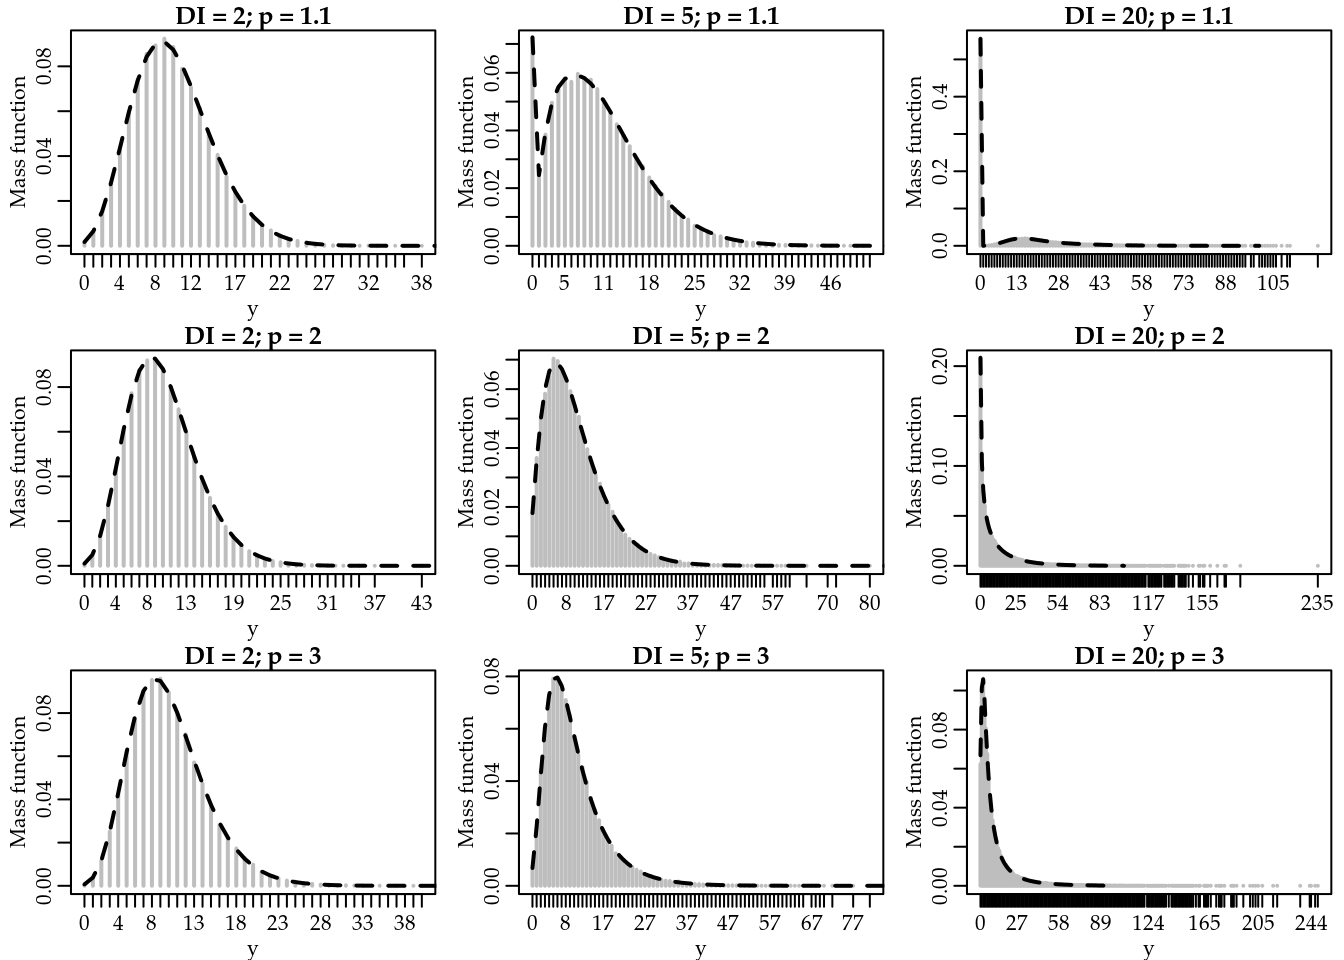
\includegraphics{rmcdbook_files/figure-latex/ptwpmfplot-1} 

}

\caption{Empirical (gray) and approximated (black) Poisson-Tweedie probability mass function by values of the dispersion index (DI) and Tweedie power parameter.}\label{fig:ptwpmfplot}
\end{figure}

For all scenarios considered the Monte Carlo method provides a quite
accurate approximation to the empirical probability mass function. For
these examples, we used \(5000\) random samples from the proposal
distribution.

Finally, the Poisson-Tweedie regression model is defined by
\[Y_i \sim PTw_{p}(\mu_i, \phi), \quad  \text{with} \quad \mu_i = g^{-1}(\boldsymbol{x_i}^{\top} \boldsymbol{\beta}),\]
where \(\boldsymbol{x}_i\) and \(\boldsymbol{\beta}\) are
\((p \times 1)\) vectors of known covariates and unknown regression
parameters. The estimation and inference of Poisson-Tweedie regression
models based on the maximum likelihood method are challenged by the
presence of an intractable integral in the probability mass function and
non-trivial restrictions on the power parameter space. In Chapter
\ref{likelihood}, we discuss maximum likelihood estimation for
Poisson-Tweedie regression. Furthermore, in Chapter \ref{SM} we extended
the Poisson-Tweedie model by using an estimating function approach in
the style of \citet{Wedderburn1974}.

\section{COM-Poisson distribution}\label{com-poisson-distribution}

The COM-Poisson distribution belongs to the family of weighted Poisson
distributions. A random variable \(Y\) is a weighted Poisson
distribution if its probability mass function can be written in the form
\[
f(y; \lambda, \nu) = \frac{\exp^{\{-\lambda\}} \lambda^y w_y}{W y!},
\quad y = 0, 1, \ldots,
\] where
\(W = \sum_{i = 0}^{\infty} \exp^{\{-\lambda\}} \lambda^i w_i / i!\) is
a normalizing constant \citep{Sellers2012}. The COM-Poisson is obtained
when \(w_{y} = (y!)^{1-\nu}\) for \(\nu \geq 0\). The series \(W\) for
COM-Poisson distribution is denoted by \(Z(\lambda, \nu)\) and can be
written as \(\sum_{i=0}^{\infty}\lambda^i/(i!)^\nu\). Note that the
series is theoretically divergent only when \(\nu = 0\) and
\(\lambda \geq 1\), but numerically for small values of \(\nu\) combined
with large values of \(\lambda\), the sum is so huge it causes overflow.
The Table \ref{tab:convergenceZ} shows the sums calculated with \(1000\)
increments, in other words, \(\sum_{i=0}^{1000}\lambda^i/(i!)^\nu\) for
different values of \(\nu\) (horizontal lines) and \(\lambda\) (vertical
lines).

\begin{table}

\caption{\label{tab:convergenceZ}Values for $Z(\lambda, \nu)$ constant (calculated numerically) to combined values of $\lambda$ (0.5 to 50) and $\phi$ (0 to 1)}
\centering
\begin{tabular}[t]{lcccccc}
\toprule
  & 0.5 & 1 & 5 & 10 & 30 & 50\\
\midrule
0 & 2.00 & Inf & Inf & Inf & Inf & Inf\\
0.1 & 1.92 & 7.64 & Inf & Inf & Inf & Inf\\
0.2 & 1.86 & 5.25 & 3.17e+273 & Inf & Inf & Inf\\
0.3 & 1.81 & 4.32 & 1.60e+29 & 2.54e+282 & Inf & Inf\\
0.4 & 1.77 & 3.80 & 4.71e+10 & 1.33e+56 & Inf & Inf\\
0.5 & 1.74 & 3.47 & 1.34e+06 & 3.67e+22 & 3.32e+196 & Inf\\
0.6 & 1.72 & 3.23 & 2.05e+04 & 4.99e+12 & 1.73e+76 & 4.63e+177\\
0.7 & 1.70 & 3.06 & 2.37e+03 & 3.69e+08 & 4.93e+39 & 6.93e+81\\
0.8 & 1.68 & 2.92 & 6.49e+02 & 2.70e+06 & 5.09e+24 & 3.43e+46\\
0.9 & 1.66 & 2.81 & 2.74e+02 & 1.47e+05 & 1.80e+17 & 2.19e+30\\
1 & 1.65 & 2.72 & 1.48e+02 & 2.20e+04 & 1.07e+13 & 5.18e+21\\
\bottomrule
\end{tabular}
\end{table}

In general, the expectation and variance of the COM-Poisson distribution
cannot be expressed in closed-form. However, they can be approximated by
\[\mathrm{E}(Y) \approx \lambda^{1/\nu} - \frac{\nu - 1}{2 \nu}
\quad \text{and} \quad
\mathrm{var}(Y) \approx \frac{1}{\nu} \lambda^{1 /\nu}.
\] These approximations are accurate when \(\nu \leq 1\) or
\(\lambda > 10^{\nu}\). The infinite sum involved in computing the
probability mass function of the COM-Poisson distribution can be
approximated to any level of precision. It can be evaluated in
\texttt{R} using the function \texttt{dcom()} from the
\texttt{compoisson} package \citep{Dunn2012}. Figure
\ref{fig:comPoispmfplot} presents some COM-Poisson probability mass
functions. We tried to find parameters \(\lambda\) and \(\nu\) in order
to have \(\mathrm{E}(Y) = 10\) and dispersion index equals to
\(\mathrm{DI} = 0.5, 2, 5\) and \(20\). However, we could not find any
parameter combination to have \(\mathrm{DI} = 20\). Probably, it was due
to overflow of the sum since \(\nu\) is inversely proportional to the
dispersion index (see table \ref{tab:convergenceZ}).

\begin{figure}[h]

{\centering 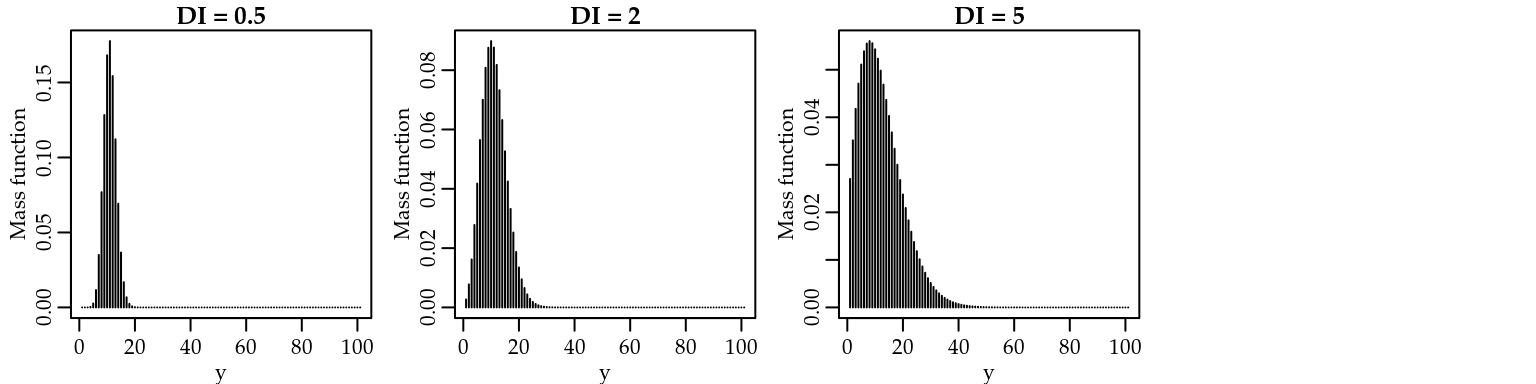
\includegraphics{rmcdbook_files/figure-latex/comPoispmfplot-1} 

}

\caption{COM-Poisson probability mass function by values of the dispersion index (DI).}\label{fig:comPoispmfplot}
\end{figure}

\citet{Sellers2010} proposed a regression model based on the COM-Poisson
distribution where the parameter \(\lambda\) is described by the values
of known covariates in a generalized linear models style. The
COM-Poisson regression model is defined by
\[Y_i \sim CP(\lambda_i, \nu), \quad  \text{with} \quad \lambda_i = g^{-1}(\boldsymbol{x_i}^{\top} \boldsymbol{\beta}).\]
In this notation, the parameter \(\nu\) is considered the dispersion
parameter such that \(\nu > 1\) represents underdispersion and
\(\nu < 1\) overdispersion. The Poisson model is obtained for
\(\nu = 1\) and as usual we adopt the logarithm link function for \(g\).

\section{Comparing count
distributions}\label{comparing-count-distributions}

Let \(Y\) be a count random variable and \(\mathrm{E}(Y) = \mu\) and
\(\mathrm{var}(Y)\) denote its mean and variance, respectively. To
explore and compare the flexibility of the models aforementioned, we
introduce the dispersion \((\mathrm{DI})\), zero-inflation
\((\mathrm{ZI})\) and heavy-tail \((\mathrm{HT})\) indexes, which are
respectively given by

\begin{equation}
\mathrm{DI} = \frac{\mathrm{var}(Y)}{\mathrm{E}(Y)}, \quad
\mathrm{ZI} = 1 + \frac{\log \mathrm{P}(Y = 0)}{\mathrm{E}(Y)}
\end{equation}

and

\begin{equation}
\mathrm{HT} = \frac{\mathrm{P}(Y=y+1)}{\mathrm{P}(Y=y)}\quad \text{for} \quad y \to \infty.
\end{equation}

These indexes are defined in relation to the Poisson distribution. Thus,
the dispersion index indicates underdispersion for \(\mathrm{DI} < 1\),
equidispersion for \(\mathrm{DI} = 1\) and overdispersion for
\(\mathrm{DI} > 1\). Similarly, the zero-inflation index is easily
interpreted, since \(\mathrm{ZI} < 0\) indicates zero-deflation,
\(\mathrm{ZI} = 0\) corresponds to no excess of zeroes and
\(\mathrm{ZI} > 0\) indicates zero-inflation. Finally,
\(\mathrm{HT} \to 1\) when \(y \to \infty\) indicates a heavy tail
distribution.

For the Poisson distribution the dispersion index equals \(1\)
\(\forall \mu\). In the Poisson case, it is easy to show that
\(\mathrm{ZI} = 0\) and \(\mathrm{HT} \to 0\) when \(y \to \infty\).
Thus, it is quite clear that the Poisson model can deal only with
equidispersed data and has no flexibility to deal with zero-inflation
and/or heavy tail count data. In fact, the presented indexes were
proposed in relation to the Poisson distribution in order to highlight
its limitations.

Figure \ref{fig:indexes} presents the relationship between mean and
variance, the dispersion and zero-inflation indexes as a function of the
expected values \(\mu\) for different scenarios and count distributions.
Scenario \(1\) corresponds to the case of underdispersion. Thus, we
fixed the dispersion index at \(\mathrm{DI} = 0.5\) when the mean
equalling \(10\). Since the Poisson-Tweedie cannot deal with
underdispersion, in this scenario we present only the Gamma-Count and
COM-Poisson distributions. Similarly, scenarios \(2--4\) are obtained by
fixing the dispersion index at \(\mathrm{DI} = 2, 5\) and \(10\) when
mean equalling \(10\). In the scenario \(4\) we could not find a
parameter configuration in order to have a COM-Poisson distribution with
dispersion index equals \(20\). Consequently, we present results only
for the Gamma-Count and Poisson-Tweedie distributions. Furthermore,
Figure \ref{fig:heavytail} presents the heavy tail index for some
extreme values of the random variable \(Y\).

\begin{figure}[h]

{\centering 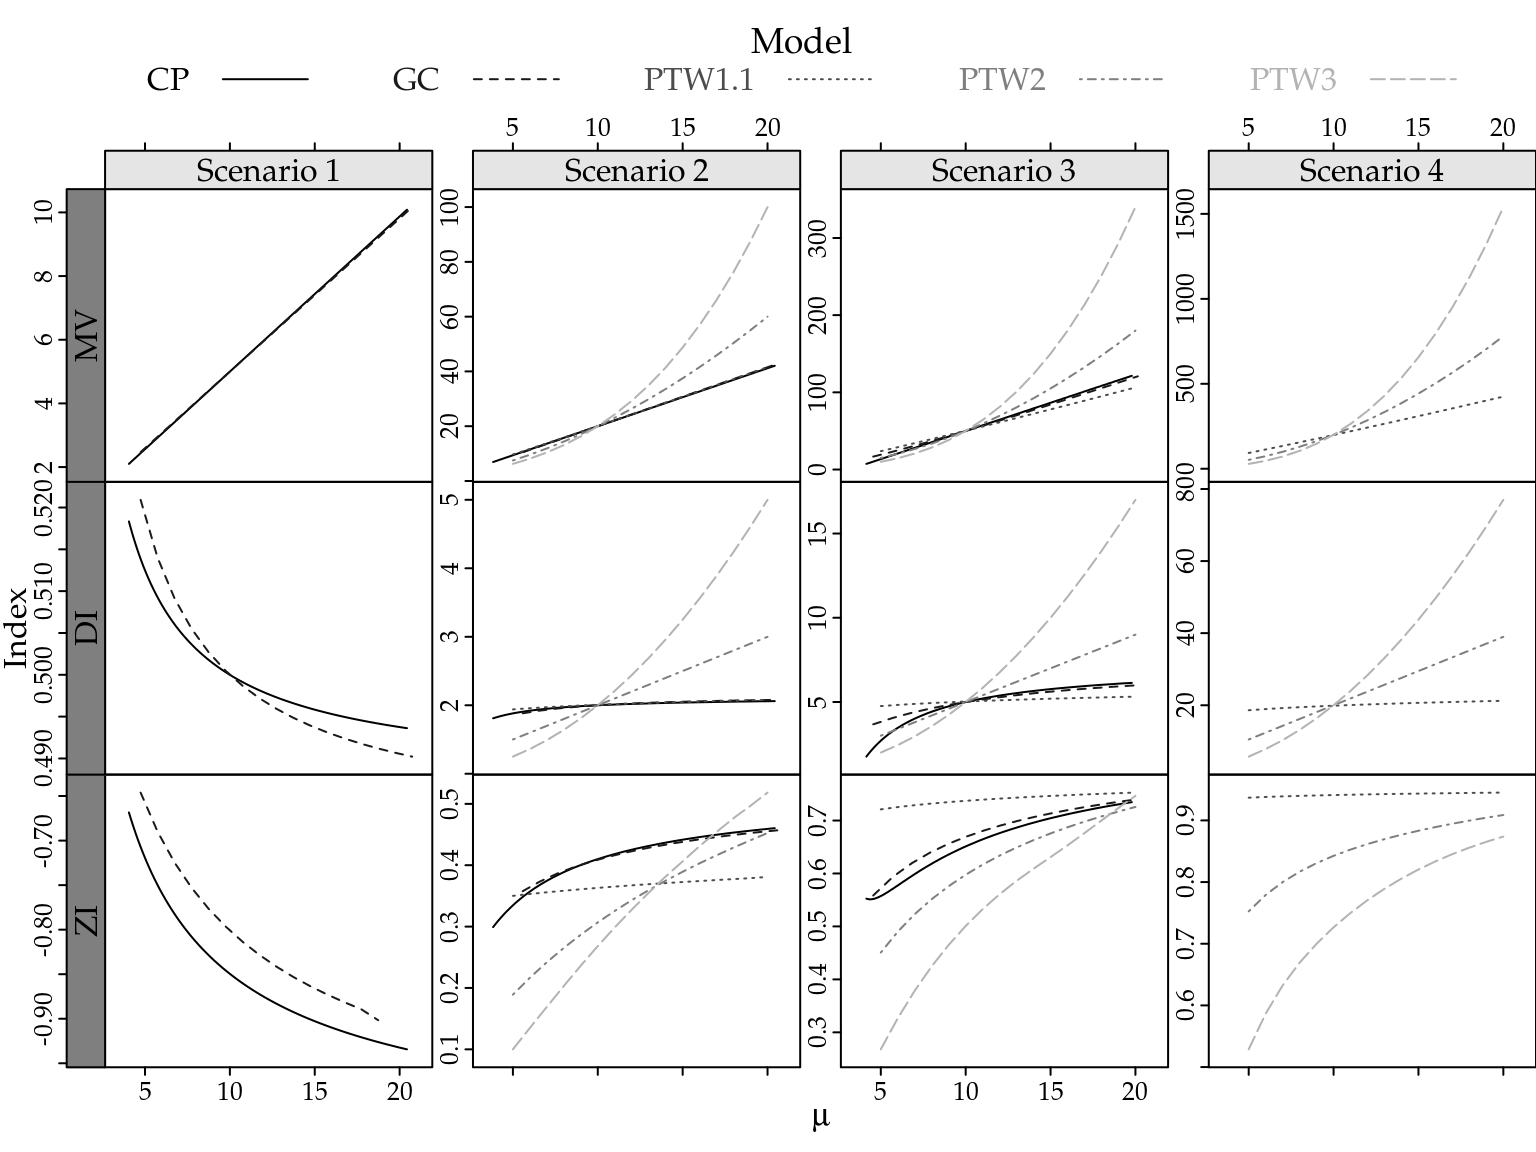
\includegraphics{rmcdbook_files/figure-latex/indexes-1} 

}

\caption{Mean and variance relationship (first line), dispersion (DI) and zero-inflation (ZI) indexes as a function of the expected values by simulation scenarios and count distributions.}\label{fig:indexes}
\end{figure}

\begin{figure}[h]

{\centering 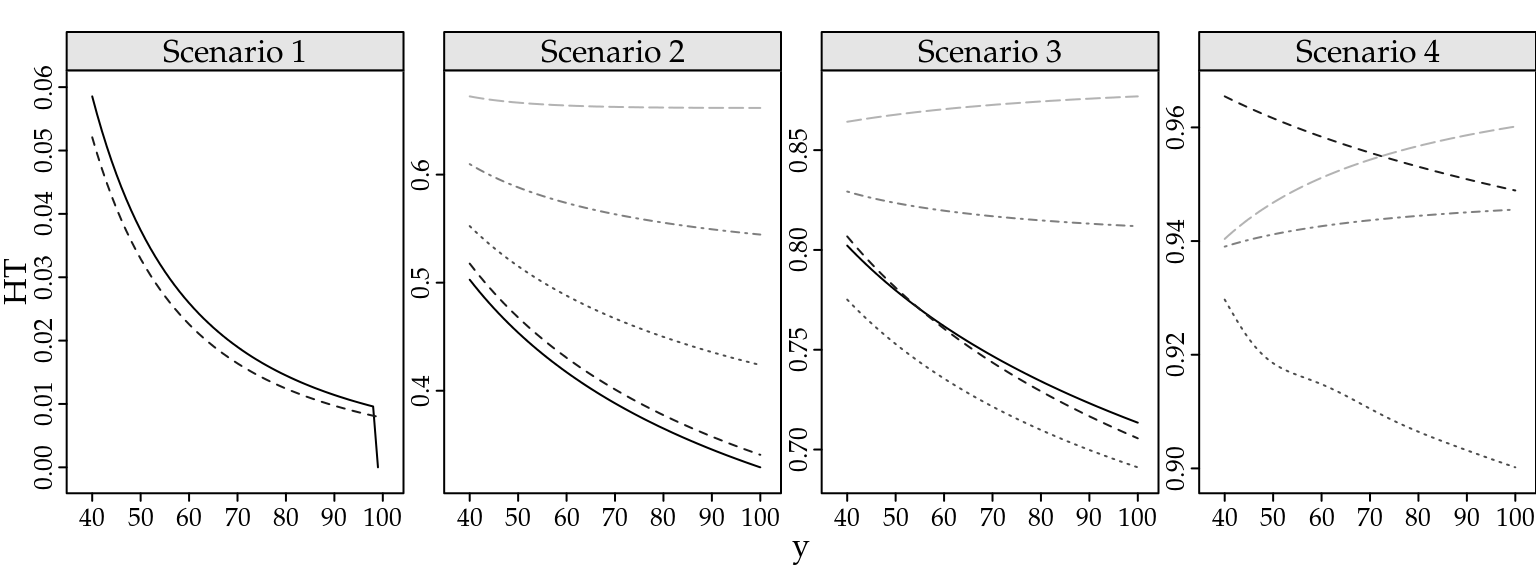
\includegraphics{rmcdbook_files/figure-latex/heavytail-1} 

}

\caption{Heavy tail index for some extreme values of the random variable Y by simulation scenarios and count distributions.}\label{fig:heavytail}
\end{figure}

The indexes presented in Figures \ref{fig:indexes} and
\ref{fig:heavytail} show that for all considered scenarios the
Gamma-Count and COM-Poisson distributions are quite similar. In general,
for these distributions, the indexes slightly depend on the expected
values and tend to stabilize for large values of \(\mu\). Consequently,
the mean and variance relationship is proportional to the dispersion
parameter value. In the overdispersion case, the Gamma-Count and
COM-Poisson distributions can handle with a limited amount of
zero-inflation and are in general light tailed distributions, i.e.
\(\mathrm{HT} \to 0\) for \(y \to \infty\).

Regarding the Poisson-Tweedie distributions the indexes show that for
small values of the power parameter the Poisson-Tweedie distribution is
suitable to deal with zero-inflated count data. In that case, the
\(\mathrm{DI}\) and \(\mathrm{ZI}\) are almost not dependent on the
values of the mean. Furthermore, the \(\mathrm{HT}\) decreases as the
mean increases. On the other hand, for large values of the power
parameter the \(\mathrm{HT}\) increases with increasing mean, showing
that the model is specially suitable to deal with heavy-tailed count
data. In this case, the \(\mathrm{DI}\) and \(\mathrm{ZI}\) increase
quickly as the mean increases giving an extremely overdispersed model
for large values of the mean. In general, the \(\mathrm{DI}\) and
\(\mathrm{ZI}\) are larger than one and zero, respectively, which, of
course, show that the corresponding Poisson-Tweedie distributions cannot
deal with underdispersed and zero-deflated count data.

For multi-parameter probability function, a desirable feature is the
orthogonality betweens parameters. This property leds a series of
statistical implications as allows make inference for one parameter
without worrying about the values of the other and computationally
numerical methods for adjusting distributions with orthogonal parameters
are more stable and fast.

The orthogonality is defined by second derivatives of the log-likelihood
function, however for the Gamma-Count, Poisson-Tweedie and COM-Poisson
and we cannot obtain such derivatives analytically. So we designed a
simulation study to evaluate the properties about log-likelihood
function for Gamma-Count and COM-Poisson. We used sample size \(n=5000\)
for simulate values of Gamma-Count and COM-Poisson following dispersion
indexes \(DI=0.5\), \(2\), \(5\) and \(20\) and plot the deviance
contours around the maximum likelihood estimation. The
\texttt{Script6.R}, in supplement material contains the codes for
simulation study. The results are shows in Figure @(fig:ortho).

This graphics presented in Figure \ref{fig:ortho} show that deviance
contours are similar a quadratic function (blue dashed contours) for
\(DI=0.5\), \(2\), \(5\) in both distributions. However, for the
Gamma-Count with \(DI=20\) the quadratic aproximation not as good. For
\(DI=20\) and \(\mathrm{E}[Y]=10\) we could not find any parameter
combination for COM-Poisson and for Gamma-Count the estimation is
innacurate. With respect to orthogonality the Gamma-Count distribution
is preferable, the deviance contours are well-behaved, while for
COM-Poisson the contour are strongly flat in one direction making the
estimation process difficult..

\begin{figure}[h]

{\centering 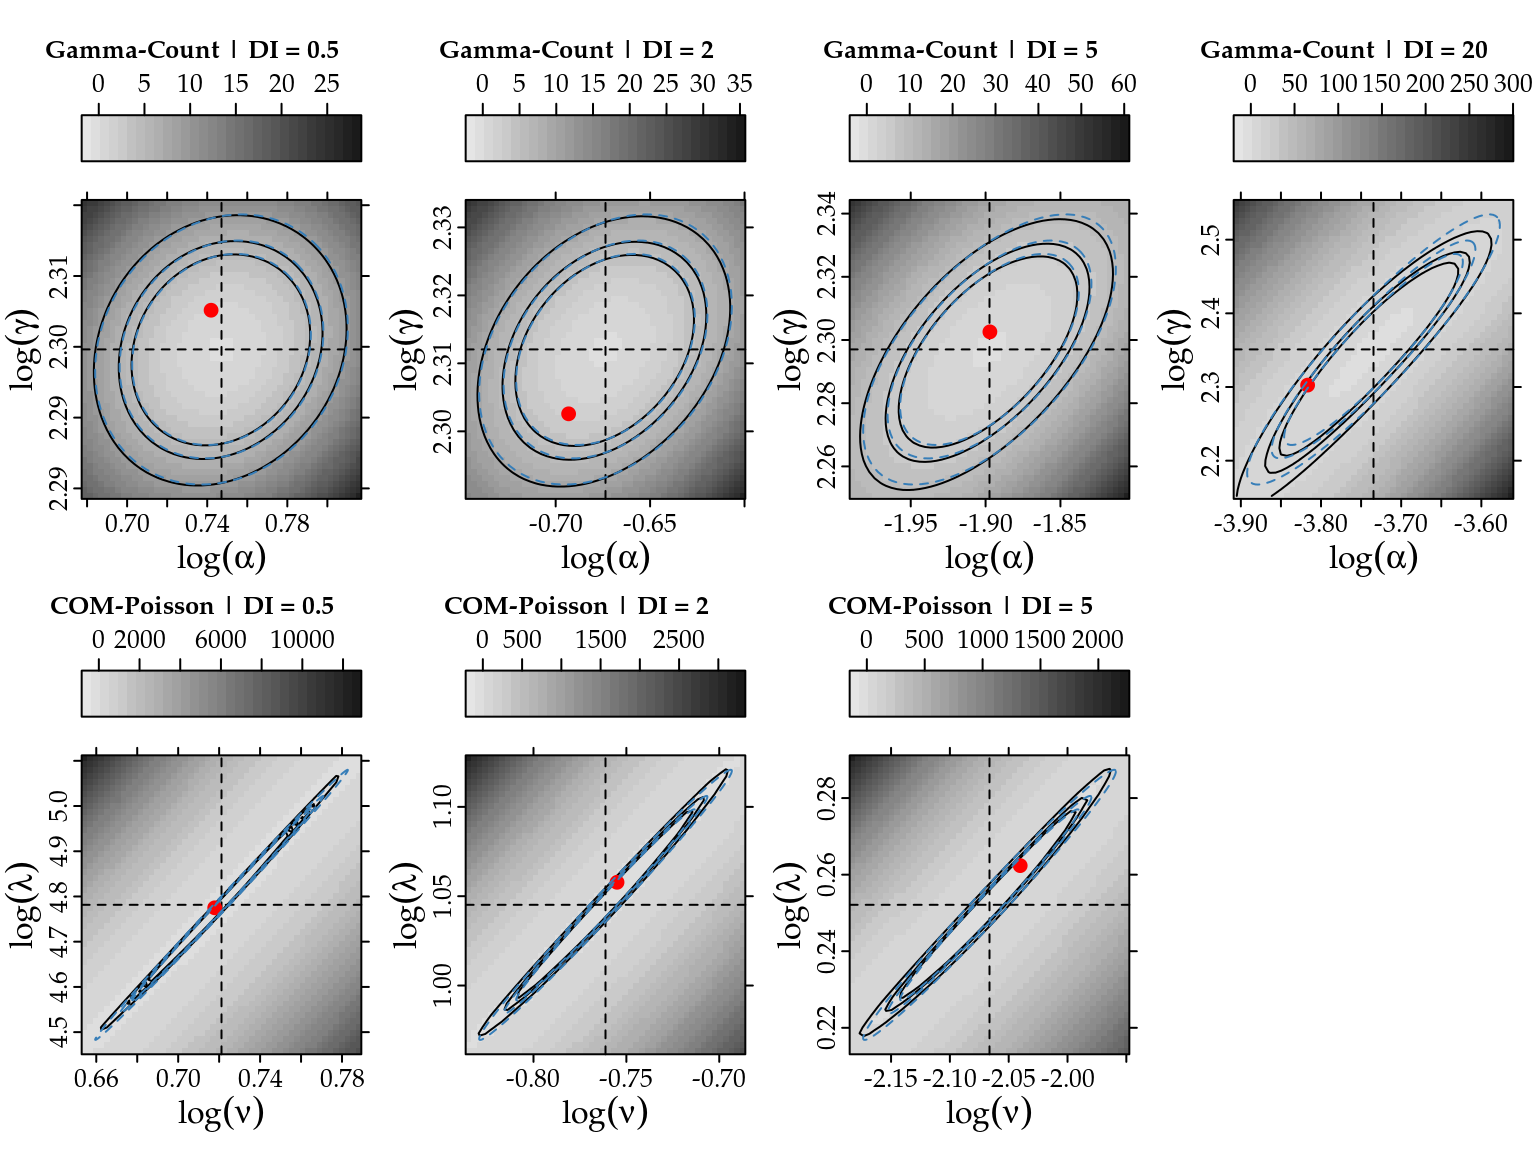
\includegraphics{rmcdbook_files/figure-latex/ortho-1} 

}

\caption{Deviance surfaces and quadratic approximation with confidence regions (90, 95 and, 99\%) for the two parameters following dispersion indexes (DI) in the simulation study. Dashed lines represents the MLE estimation and red points the parameters used in simulation.}\label{fig:ortho}
\end{figure}

In terms of regression models, the Poisson and Poisson-Tweedie models
are easy and convenient to interpret because the expected value is
directly modelled as a function of known covariates in a generalized
linear models manner. On the other hand, the Gamma-Count specifies the
regression model for the expectation of the times between events and,
thus requires careful interpretation. The COM-Poisson regression model
is hard to interpret and compare with the traditional Poisson regression
model, since it specifies the regression model for the parameter
\(\lambda\) that has no easy interpretation in relation to the
expectation of the count response variable.

Finally, in terms of computational implementation the simplicity of the
Poisson regression model is unquestionable. The probability mass
function of the Gamma-Count distribution requires the evaluation of the
difference between two cumulative gamma distributions. For large values
of the random variable \(Y\), such a difference can be time consuming
and inaccurately computed. Similarly, the COM-Poisson probability mass
function involves the evaluation of a infinity sum, which can be
computational expensive and inaccurate for large values of \(Y\).
Furthermore, for extreme values of \(\lambda\) combined with small
values of \(\nu\) the infinite sum can numerically diverges making
impossible to evaluate the probability mass function. Finally, the
Poisson-Tweedie probability mass function involves an intractable
integral, which makes the estimation and inference based on likelihood
methods computationally intensive.

\chapter{The method of maximum likelihood}\label{likelihood}

The estimation and inference for the models discussed in Chapter
\ref{models} can be done by the method of maximum likelihood
\citep{Silvey:1975}. In this Chapter, we present the maximum likelihood
method and its main properties along with some examples in \texttt{R}.
The maximum likelihood method is applicable mainly in situations where
the true distribution of the count random variable \(Y\) is known apart
of the values of a finite number of unknown parameters. Let
\(f(y;\boldsymbol{\theta})\) denote the true probability mass function
of the count random variable \(Y\). We assume that the family
\(f(y;\boldsymbol{\theta})\) is labelled by a (\(p \times 1\)) parameter
vector \(\boldsymbol{\theta}\) taking values in \(\Theta\) a subset of
\(\mathbb{R}^n\). For a given observed value \(y\) of the a random
variable \(Y\), the likelihood function corresponding to the observation
\(y\) is defined as
\(L(\boldsymbol{\theta};y) = f(y;\boldsymbol{\theta})\). It is important
to highlight that \(f(y;\boldsymbol{\theta})\) is a probability mass
function on the sample space. On the other hand,
\(L(\boldsymbol{\theta};y) = f(y;\boldsymbol{\theta})\) is a function on
the parameter space \(\Theta\). The likelihood function expresses the
plausibilities of different parameters after we have observed \(y\), in
the absence of any other information that we may have about these
different values. In particular, for count random variables the
likelihood function is the probability of the point \(y\) when
\(\boldsymbol{\theta}\) is the true parameter.

The method of maximum likelihood has a strong intuitive appeal and
according to it, we estimate the true parameter \(\boldsymbol{\theta}\)
by any parameter which maximizes the likelihood function. In general,
there is a unique maximizing parameter which is the most plausible and
this is the maximum likelihood estimate \citep{Silvey:1975}. In other
words, a maximum likelihood estimate \(\hat{\boldsymbol{\theta}}(y)\) is
any element of \(\Theta\) such that
\(L(\hat{\boldsymbol{\theta}}(y);y) = \underset{\boldsymbol{\theta}\in \Theta}\max L(\boldsymbol{\theta};y).\)
At this stage, we make the distinction between the estimate
\(\hat{\boldsymbol{\theta}}(y)\) and the estimator
\(\hat{\boldsymbol{\theta}}\). However, we are not maintain this
distinction and we shall use only \(\hat{\boldsymbol{\theta}}\) leaving
the context to make it clear whether we are thinking of
\(\hat{\boldsymbol{\theta}}\) as a function or as a particular value of
a function.

Let \(Y_i\) be independent and identically distributed count random
variables with probability mass function \(f(y;\boldsymbol{\theta})\),
whose observed values are denoted by \(y_i\) for \(i = 1, \ldots, n.\)
In this case, the likelihood function can be written as the product of
the individuals probability mass distributions, i.e.

\begin{equation}
L(\boldsymbol{\theta};\boldsymbol{y}) = \prod_{i=1}^n L(\boldsymbol{\theta}; y_i) = \prod_{i=1}^n f(y_i; \boldsymbol{\theta}).
\label{eq:LIK}
\end{equation}

For convenience, in practical situations is advisable to work with the
log-likelihood function obtained by taking the logarithm of Eq.
\eqref{eq:LIK}. Thus, the maximum likelihood estimator (MLE) for the
parameter vector \(\boldsymbol{\theta}\) is obtained by maximizing the
following log-likelihood function,

\begin{equation}
\ell(\boldsymbol{\theta})=\sum^n_{i=1} \log\{ L(\boldsymbol{\theta}; y_i) \}.
\label{eq:LOGLIK}
\end{equation}

Often, it is not possible to find a relatively simple expression in
closed form for the maximum likelihood estimates. However, it is usually
possible to assume that maximum likelihood estimates emerge as a
solution of the likelihood equations or also called score functions,
i.e.

\begin{equation}
\mathcal{U}(\boldsymbol{\theta}) = \left ( \frac{\partial \ell(\boldsymbol{\theta})}{\partial \theta_1}^\top, \ldots, \frac{\partial \ell(\boldsymbol{\theta})}{\partial \theta_p}^\top \right )^\top = \boldsymbol{0}.
\label{eq:SCORE}
\end{equation}

The system of non-linear equations in \eqref{eq:SCORE} often have to be
solved numerically. The entry \((i,j)\) of the \(p \times p\) Fisher
information matrix \(\mathcal{F}_{\boldsymbol{\theta}}\) for the vector
of parameter \(\boldsymbol{\theta}\) is given by

\begin{equation}
\mathcal{F}_{\boldsymbol{\theta}_{ij}} =-\mathrm{E} \left \{ \frac{\partial^2 \ell(\boldsymbol{\theta})}{\partial\theta_i\partial\theta_j} \right \}.
\end{equation}

In order to solve the system of equations
\(\mathcal{U}(\boldsymbol{\theta}) = \boldsymbol{0}\), we employ the
Newton scoring algorithm, defined by

\begin{eqnarray}
\boldsymbol{\theta}^{(i+1)} &=& \boldsymbol{\theta}^{(i)} - \mathcal{F}_{\boldsymbol{\theta}}^{-1} \mathcal{U}(\boldsymbol{\theta}^{(i)}).
\end{eqnarray}

Finally, the well known distribution of the maximum likelihood estimator
\(\boldsymbol{\hat{\theta}}\) is
\(\mathrm{N}(\boldsymbol{\theta}, \mathcal{F}_{\boldsymbol{\theta}}^{-1})\).
Thus, the maximum likelihood estimator is asymptotically consistent,
unbiased and efficient.

A critical point of the approach described so far, is that we should be
able to compute the first and second derivatives of the log-likelihood
function. However, for the Gamma-Count where the log-likelihood function
is given by the difference between two integrals, we cannot obtain such
derivatives analytically. Similarly, for the COM-Poisson the
log-likelihood function involves an infinite sum and consequently such
derivatives cannot be obtained analytically. Finally, in the
Poisson-Tweedie distribution the log-likelihood function is defined by
an intractable integral, which implies that we cannot obtain a
closed-form for the score function and Fisher information matrix.

Thus, an alternative approach is to maximize directly the log-likelihood
function in equation \eqref{eq:LOGLIK} using a derivative-free algorithm
as the Nelder-Mead method \citep{Nelder:1965} or some other numerical
method for maximizing the log-likelihood function, examples include the
\(BFGS\), conjugate gradient and simulated annealing. All of them are
implemented in \texttt{R} through the \texttt{optim()} function. The
package \texttt{bbmle} \citep{bbmle:2014} offers a suite of functions to
work with numerical maximization of log-likelihood functions in
\texttt{R}. As an example, consider the Gamma-Count distribution
described in subsection \ref{gammacount}. The log-likelihood function
for the parameters \(\theta = (\gamma, \alpha)\) in \texttt{R} is given
by

\begin{Shaded}
\begin{Highlighting}[]
\NormalTok{ll_gc <-}\StringTok{ }\NormalTok{function(gamma, alpha, y) \{}
  \NormalTok{ll <-}\StringTok{ }\KeywordTok{sum}\NormalTok{(}\KeywordTok{dgc}\NormalTok{(}\DataTypeTok{y =} \NormalTok{y, }\DataTypeTok{gamma =} \NormalTok{gamma, }\DataTypeTok{alpha =} \NormalTok{alpha, }\DataTypeTok{log =} \OtherTok{TRUE}\NormalTok{))}
  \KeywordTok{return}\NormalTok{(-ll)}
\NormalTok{\}}
\end{Highlighting}
\end{Shaded}

Thus, for a given vector of observed count values, we can numerically
maximize the log-likelihood function above using the function
\texttt{mle2()} from the \texttt{bbmle}package. It is important to
highlight that by default the \texttt{mle2()} function requires the
negative of the log-likelihood function instead of the log-likelihood
itself. Thus, our function returns the negative value of the
log-likelihood function.

\begin{Shaded}
\begin{Highlighting}[]
\KeywordTok{require}\NormalTok{(bbmle)}
\NormalTok{y <-}\StringTok{ }\KeywordTok{rpois}\NormalTok{(}\DecValTok{100}\NormalTok{, }\DataTypeTok{lambda =} \DecValTok{10}\NormalTok{)}
\NormalTok{fit_gc <-}\StringTok{ }\KeywordTok{mle2}\NormalTok{(ll_gc, }\DataTypeTok{start =} \KeywordTok{list}\NormalTok{(}\StringTok{"gamma"} \NormalTok{=}\StringTok{ }\DecValTok{10}\NormalTok{, }\StringTok{"alpha"} \NormalTok{=}\StringTok{ }\DecValTok{1}\NormalTok{),}
               \DataTypeTok{data =} \KeywordTok{list}\NormalTok{(}\StringTok{"y"} \NormalTok{=}\StringTok{ }\NormalTok{y))}
\end{Highlighting}
\end{Shaded}

The great advantage of the \texttt{bbmle} package for maximum likelihood
estimation in \texttt{R}, is that it already provides standard methods,
such as \texttt{summary()}, \texttt{coef()}, \texttt{confint()},
\texttt{vcov()}, \texttt{profile()} and other for objects of
\texttt{mle2} class.

\begin{Shaded}
\begin{Highlighting}[]
\KeywordTok{summary}\NormalTok{(fit_gc)}
\end{Highlighting}
\end{Shaded}

\begin{verbatim}
## Maximum likelihood estimation
## 
## Call:
## mle2(minuslogl = ll_gc, start = list(gamma = 10, alpha = 1), 
##     data = list(y = y))
## 
## Coefficients:
##       Estimate Std. Error z value   Pr(z)    
## gamma    9.842      0.335   29.38 < 2e-16 ***
## alpha    0.929      0.139    6.68 2.5e-11 ***
## ---
## Signif. codes:  0 '***' 0.001 '**' 0.01 '*' 0.05 '.' 0.1 ' ' 1
## 
## -2 log L: 518
\end{verbatim}

Similar functions can be done for the Poisson, Poisson-Tweedie and
COM-Poisson distributions.

\chapter{Models specified by second-moment assumptions}\label{SM}

In Chapter \ref{models}, we presented four statistical models to deal
with count data and in the Chapter \ref{likelihood} the method of
maximum likelihood was introduced to estimate the model's parameters. As
discussed in Chapter \ref{likelihood} the method of maximum likelihood
assumes that the true distribution of the count random variable \(Y\) is
known apart of the values of a finite number of unknown parameters. In
this Chapter, we shall present a different approach for model
specification, estimation and inference based only on second-moment
assumptions.

\section{Extended Poisson-Tweedie
model}\label{extended-poisson-tweedie-model}

The Poisson-Tweedie distribution as presented in subsection \ref{ptw}
provides a very flexible family of count distributions, however, such a
family has two main drawbacks: it cannot deal with underdispersed count
data and its probability mass function is given by an intractable
integral, which implies that estimation based on the maximum likelihood
method is computational demanding for practical data analysis.

In spite of these issues \citet{Jorgensen2014} showed using factorial
cumulant function that for \(Y \sim PTw_p(\mu, \phi)\),
\(\mathrm{E}(Y) = \mu\) and \(\mathrm{var}(Y) = \mu + \phi \mu^p\). This
fact motivates \citet{Bonat2016b} to specify a model by using only
second-moment assumptions, i.e.~mean and variance.

Thus, consider a cross-section dataset, \((y_i, \boldsymbol{x}_i)\),
\(i = 1, \ldots, n\), where \(y_i\)'s are i.i.d. realizations of \(Y_i\)
according to an unspecified distribution, whose expectation and variance
are given by

\begin{align}
\mathrm{E}(Y_i) = \mu_i = g^{-1}(\boldsymbol{x}_i^{\top} \boldsymbol{\beta}) \nonumber \\
\mathrm{var}(Y_i) = C_i = \mu_i + \phi \mu_i^p,
\label{eq:EPTW}
\end{align}

where as before \(\boldsymbol{x}_i\) and \(\boldsymbol{\beta}\) are
(\(p \times 1\)) vectors of known covariates and unknown regression
parameters and \(g\) is the logarithm link function. The regression
model specified in \eqref{eq:EPTW} is parametrized by
\(\boldsymbol{\theta} = (\boldsymbol{\beta}^\top, \boldsymbol{\lambda}^\top )^\top\),
where \(\boldsymbol{\lambda} = (\phi, p)\).

Note that, based on second-moment assumptions, the only restriction to
have a proper model is that \(\mathrm{var}(Y_i) > 0\), thus
\[\phi > - \mu^{(1-p)}_i,\] which shows that at least at some extent
negative values for the dispersion parameter are allowed. Consequently,
the Poisson-Tweedie model can be extended to deal with underdispersed
count data, however, in doing so the associated probability mass
functions do not exist. However, in a regression modelling framework as
discussed in this material, we are in general interested in the
regression coefficient effects, thus such an issue does not imply any
loss of interpretation and applicability. The formulation of the
extended Poisson-Tweedie model is exactly the same of the quasi-binomial
and quasi-Poisson models popular in the context of generalized linear
models, see \citep[\citet{Nelder1972}]{Wedderburn1974} for details.
Furthermore, note that for \(p = 1\) the extended Poisson-Tweedie
regression model corresponds to a reparametrization of the popular
quasi-Poisson regression model.

It is also important to highlight that in this case the relationship
between mean and variance is proportional to the dispersion parameter
\(\phi\) as in the Gamma-Count and COM-Poisson distributions. Thus, we
expect for \(\phi < 0\) and \(p = 1\) the extended Poisson-Tweedie model
presents results in terms of regression coefficients really similar the
ones from the Gamma-Count and COM-Poisson regression models.

\section{Estimation and Inference}\label{estimation-and-inference}

Since the model presented in \eqref{eq:EPTW} is based only on
second-moment assumptions the method of maximum likelihood cannot be
employed. \citet{Bonat2016b} based on ideas of \citet{Jorgensen2004} and
\citet{Bonat2016a} proposed an estimating function approach for
estimation and inference for the extended Poisson-Tweedie regression
model. \citet{Bonat2016b} combined the quasi-score and Pearson
estimating functions for estimation of the regression and dispersion
parameters respectively. Following \citet{Bonat2016b} the quasi-score
function for \(\boldsymbol{\beta}\) has the following form,

\begin{equation*}
\psi_{\boldsymbol{\beta}}(\boldsymbol{\beta}, \boldsymbol{\lambda}) = \left (\sum_{i=1}^n \frac{\partial \mu_i}{\partial \beta_1}C^{-1}_i(Y_i - \mu_i), \ldots, \sum_{i=1}^n \frac{\partial \mu_i}{\partial \beta_p}C^{-1}_i(Y_i - \mu_i)  \right )^\top,
\end{equation*}

where \(\partial \mu_i/\partial \beta_j = \mu_i x_{ij}\) for
\(j = 1, \ldots, p\). The sensitivity matrix is defined as the
expectation of the first derivative of the estimating function with
respect to the model parameters. Thus, the entry \((j,k)\) of the
\(p \times p\) sensitivity matrix for \(\psi_{\boldsymbol{\beta}}\) is
given by

\begin{equation}
\mathrm{S}_{\boldsymbol{\beta}_{jk}} = \mathrm{E}\left ( \frac{\partial}{\partial \beta_k} \psi_{\boldsymbol{\beta}_j}(\boldsymbol{\beta}, \boldsymbol{\lambda})  \right ) = -\sum_{i=1}^n \mu_i x_{ij} C^{-1}_i x_{ik} \mu_i.
\label{eq:Sbeta}
\end{equation}

In a similar way, the variability matrix is defined as the variance of
the estimating function. In particular, for the quasi-score function the
entry \((j,k)\) of the \(p \times p\) variability matrix is given by

\begin{equation*}
\label{Vbeta}
\mathrm{V}_{\boldsymbol{\beta}_{jk}} = \mathrm{Cov}(\psi_{\boldsymbol{\beta}_j}(\boldsymbol{\beta}, \boldsymbol{\lambda}),\psi_{\boldsymbol{\beta}_k}(\boldsymbol{\beta}, \boldsymbol{\lambda})) = \sum_{i=1}^n \mu_i x_{ij} C^{-1}_i x_{ik} \mu_i.
\end{equation*}

The Pearson estimating function for the dispersion parameters has the
following form,

\begin{equation*}
\label{Pearson}
\psi_{\boldsymbol{\lambda}}(\boldsymbol{\lambda}, \boldsymbol{\beta}) = \left (-\sum_{i=1}^n \frac{\partial C^{-1}_i}{\partial \phi} \left [ (Y_i - \mu_i)^2 - C_i \right ], -\sum_{i=1}^n \frac{\partial C^{-1}_i}{\partial p}  \left [ (Y_i - \mu_i)^2 - C_i \right ]  \right )^\top.
\end{equation*}

Note that, the Pearson estimating functions are unbiased estimating
functions for \(\boldsymbol{\lambda}\) based on the squared residuals
\((Y_i - \mu_i)^2\) with expected value \(C_i\).

The entry \((j,k)\) of the \(2 \times 2\) sensitivity matrix for the
dispersion parameters is given by

\begin{equation}
\mathrm{S}_{\boldsymbol{\lambda}_{jk}} = \mathrm{E}\left ( \frac{\partial}{\partial \lambda_k}\psi_{\boldsymbol{\lambda}_j}(\boldsymbol{\lambda}, \boldsymbol{\beta})  \right ) = -\sum_{i=1}^n \frac{\partial C^{-1}_i}{\partial \lambda_j} C_i \frac{\partial C^{-1}_i}{\partial \lambda_k}C_i,
\label{eq:Slambda}
\end{equation}

where \(\lambda_1\) and \(\lambda_2\) denote either \(\phi\) or \(p\).

Similarly, the cross entries of the sensitivity matrix are given by

\begin{equation}
\mathrm{S}_{\boldsymbol{\beta}_j \boldsymbol{\lambda}_k} = \mathrm{E}\left ( \frac{\partial}{\partial \lambda_k}\psi_{\boldsymbol{\beta}_j}(\boldsymbol{\beta}, \boldsymbol{\lambda})  \right ) = 0
\label{eq:Sbetalambda}
\end{equation}

and

\begin{equation}
\mathrm{S}_{\boldsymbol{\lambda}_j \boldsymbol{\beta}_k} = \mathrm{E}\left ( \frac{\partial}{\partial \beta_k}\psi_{\boldsymbol{\lambda}_j}(\boldsymbol{\lambda}, \boldsymbol{\beta})  \right ) = -\sum_{i=1}^n \frac{\partial C_i^{-1}}{\partial \lambda_j} C_i \frac{\partial C_i^{-1}}{\partial \beta_k} C_i.
\label{eq:Slambdabeta}
\end{equation}

Finally, the joint sensitivity matrix for the parameter vector
\(\boldsymbol{\theta}\) is given by

\begin{equation*}
\mathrm{S}_{\boldsymbol{\theta}} = \begin{pmatrix}
\mathrm{S}_{\boldsymbol{\beta}} & \boldsymbol{0} \\
\mathrm{S}_{\boldsymbol{\lambda}\boldsymbol{\beta}} & \mathrm{S}_{\boldsymbol{\lambda}}
\end{pmatrix},
\end{equation*}

whose entries are defined by equations \eqref{eq:Sbeta}, \eqref{eq:Slambda},
\eqref{eq:Sbetalambda} and \eqref{eq:Slambdabeta}.

We now calculate the asymptotic variance of the estimating function
estimators denoted by \(\boldsymbol{\hat{\theta}}\), as obtained from
the inverse Godambe information matrix, whose general form for a vector
of parameter \(\boldsymbol{\theta}\) is
\(\mathrm{J}^{-1}_{\boldsymbol{\theta}} = \mathrm{S}^{-1}_{\boldsymbol{\theta}} \mathrm{V}_{\boldsymbol{\theta}} \mathrm{S}^{-\top}_{\boldsymbol{\theta}}\),
where \(-\top\) denotes inverse transpose. The variability matrix for
\(\boldsymbol{\theta}\) has the form

\begin{equation}
\mathrm{V}_{\boldsymbol{\theta}} = \begin{pmatrix}
\mathrm{V}_{\boldsymbol{\beta}} & \mathrm{V}_{\boldsymbol{\beta}\boldsymbol{\lambda}} \\
\mathrm{V}_{\boldsymbol{\lambda}\boldsymbol{\beta}} & \mathrm{V}_{\boldsymbol{\lambda}}
\end{pmatrix},
\label{eq:VTHETA}
\end{equation}

where
\(\mathrm{V}_{\boldsymbol{\lambda}\boldsymbol{\beta}} = \mathrm{V}^{\top}_{\boldsymbol{\beta}\boldsymbol{\lambda}}\)
and \(\mathrm{V}_{\boldsymbol{\lambda}}\) depend on the third and fourth
moments of \(Y_i\), respectively. In order to avoid this dependence on
higher-order moments, we use the empirical versions of
\(\mathrm{V}_{\boldsymbol{\lambda}}\) and
\(\mathrm{V}_{\boldsymbol{\lambda}\boldsymbol{\beta}}\) as given by

\begin{equation*}
\tilde{\mathrm{V}}_{\boldsymbol{\lambda}_{jk}} = \sum_{i=1}^n \psi_{\boldsymbol{\lambda}_j}(\boldsymbol{\lambda}, \boldsymbol{\beta})_i\psi_{\boldsymbol{\lambda}_k}(\boldsymbol{\lambda}, \boldsymbol{\beta})_i \quad \text{and} \quad \tilde{\mathrm{V}}_{\boldsymbol{\lambda}_j \boldsymbol{\beta}_k} = \sum_{i=1}^n \psi_{\boldsymbol{\lambda}_j}(\boldsymbol{\lambda}, \boldsymbol{\beta})_i \psi_{\boldsymbol{\beta}_k}(\boldsymbol{\lambda}, \boldsymbol{\beta})_i.
\end{equation*}

Finally, the well known asymptotic distribution of
\(\boldsymbol{\hat{\theta}}\) \citep{Jorgensen2004} is given by

\begin{equation*}
\boldsymbol{\hat{\theta}} \sim \mathrm{N}(\boldsymbol{\theta}, \mathrm{J}_{\boldsymbol{\theta}}^{-1}), \quad \text{where} \quad
\mathrm{J}^{-1}_{\boldsymbol{\theta}} = \mathrm{S}^{-1}_{\boldsymbol{\theta}} \mathrm{V}_{\boldsymbol{\theta}} \mathrm{S}^{-\top}_{\boldsymbol{\theta}}.
\end{equation*}

To solve the system of equations
\(\psi_{\boldsymbol{\beta}} = \boldsymbol{0}\) and
\(\psi_{\boldsymbol{\lambda}} = \boldsymbol{0}\) \citet{Jorgensen2004}
proposed the modified chaser algorithm, defined by

\begin{eqnarray*}
\label{chaser}
\boldsymbol{\beta}^{(i+1)} &=& \boldsymbol{\beta}^{(i)} - \mathrm{S}_{\boldsymbol{\beta}}^{-1} \psi_{\boldsymbol{\beta}}(\boldsymbol{\beta}^{(i)}, \boldsymbol{\lambda}^{(i)}) \nonumber \\
\boldsymbol{\lambda}^{(i+1)} &=& \boldsymbol{\lambda}^{(i)} - \alpha \mathrm{S}_{\boldsymbol{\lambda}}^{-1} \psi_{\boldsymbol{\lambda}}(\boldsymbol{\beta}^{(i+1)}, \boldsymbol{\lambda}^{(i)}).
\end{eqnarray*}

The modified chaser algorithm uses the insensitivity property
\eqref{eq:Sbetalambda}, which allows us to use two separate equations to
update \(\boldsymbol{\beta}\) and \(\boldsymbol{\lambda}\). We introduce
the tuning constant, \(\alpha\), to control the step-length. This
algorithm is a special case of the flexible algorithm presented by
\citet{Bonat2016a} in the context of multivariate covariance generalized
linear models. Hence, estimation for the extended Poisson-Tweedie model
is easily implemented in \texttt{R} through the \texttt{mcglm}
\citep{Bonat2016c} package.

\chapter{Applications}\label{applications}

In this chapter, we will bring some applications based on real data sets
to show how use R packages to analyse count data.

\section{Cotton Bolls}\label{cotton-bolls}

Cotton production can be drastically reduced by attack of defoliating
insects. Depending on the growth stage, the plant can recover from the
caused damage and keeps production not affected or can have the
production reduced by low intensity defoliation.

A greenhouse experiment with cotton plants (\emph{Gossypium hirsutum})
was done under a completely randomized design with five replicates to
assess the effects of five defoliation levels (0\%, 25\%, 50\%,75\% and
100\%) on the observed number of bolls produced by plants at five growth
stages: vegetative, flower-bud, blossom, fig and cotton boll. The
experimental unity was a pot with two plants \citep[for
more]{Silva2012a}. The number of cotton bolls was recorded at the
hasvest of the experiment.

\begin{Shaded}
\begin{Highlighting}[]
\KeywordTok{library}\NormalTok{(lattice)}
\KeywordTok{library}\NormalTok{(latticeExtra)}
\KeywordTok{library}\NormalTok{(gridExtra)}
\KeywordTok{library}\NormalTok{(plyr)}
\KeywordTok{library}\NormalTok{(car)}
\KeywordTok{library}\NormalTok{(corrplot)}
\KeywordTok{library}\NormalTok{(doBy)}
\KeywordTok{library}\NormalTok{(multcomp)}
\KeywordTok{library}\NormalTok{(mcglm)}
\KeywordTok{library}\NormalTok{(MRDCr)}
\KeywordTok{ls}\NormalTok{(}\StringTok{"package:MRDCr"}\NormalTok{)}
\end{Highlighting}
\end{Shaded}

\begin{verbatim}
##  [1] "apc"                  "calc_mean_cmp"       
##  [3] "calc_mean_gcnt"       "calc_var_cmp"        
##  [5] "cambras"              "capdesfo"            
##  [7] "capmosca"             "cmp"                 
##  [9] "conftemp"             "confterm"            
## [11] "convergencez"         "dcmp"                
## [13] "dgcnt"                "dpgnz"               
## [15] "gcnt"                 "led"                 
## [17] "llcmp"                "llgcnt"              
## [19] "llpgnz"               "nematoide"           
## [21] "ninfas"               "panel.beeswarm"      
## [23] "panel.cbH"            "panel.groups.segplot"
## [25] "peixe"                "pgnz"                
## [27] "postura"              "prepanel.cbH"        
## [29] "seguros"              "soja"
\end{verbatim}

\begin{Shaded}
\begin{Highlighting}[]
\CommentTok{# Documentation in Portuguese.}
\KeywordTok{help}\NormalTok{(capdesfo, }\DataTypeTok{help_type =} \StringTok{"html"}\NormalTok{)}
\end{Highlighting}
\end{Shaded}

\begin{Shaded}
\begin{Highlighting}[]
\KeywordTok{str}\NormalTok{(capdesfo)}
\end{Highlighting}
\end{Shaded}

\begin{verbatim}
## 'data.frame':    125 obs. of  4 variables:
##  $ est : Factor w/ 5 levels "vegetativo","botão floral",..: 1 1 1 1 1 1 1 1 1 1 ...
##  $ des : num  0 0 0 0 0 0.25 0.25 0.25 0.25 0.25 ...
##  $ rept: int  1 2 3 4 5 1 2 3 4 5 ...
##  $ ncap: int  10 9 8 8 10 11 9 10 10 10 ...
\end{verbatim}

\begin{Shaded}
\begin{Highlighting}[]
\KeywordTok{levels}\NormalTok{(capdesfo$est) <-}\StringTok{ }\KeywordTok{c}\NormalTok{(}\StringTok{"vegetative"}\NormalTok{,}
                          \StringTok{"flower-bud"}\NormalTok{,}
                          \StringTok{"blossom"}\NormalTok{,}
                          \StringTok{"fig"}\NormalTok{,}
                          \StringTok{"cotton boll"}\NormalTok{)}
\KeywordTok{xtabs}\NormalTok{(~est +}\StringTok{ }\NormalTok{des, }\DataTypeTok{data =} \NormalTok{capdesfo)}
\end{Highlighting}
\end{Shaded}

\begin{verbatim}
##              des
## est           0 0.25 0.5 0.75 1
##   vegetative  5    5   5    5 5
##   flower-bud  5    5   5    5 5
##   blossom     5    5   5    5 5
##   fig         5    5   5    5 5
##   cotton boll 5    5   5    5 5
\end{verbatim}

Figure \ref{fig:bools-mean-var} (top) shows the beeswarm plot of number
of cotton bolls recorded for each combination of defoliation level and
growth stage. All the points in the sample means and variances
dispersion diagram (bottom) are below the identity line, clearly
suggesting data with underdispersion.

\begin{figure}[h]

{\centering 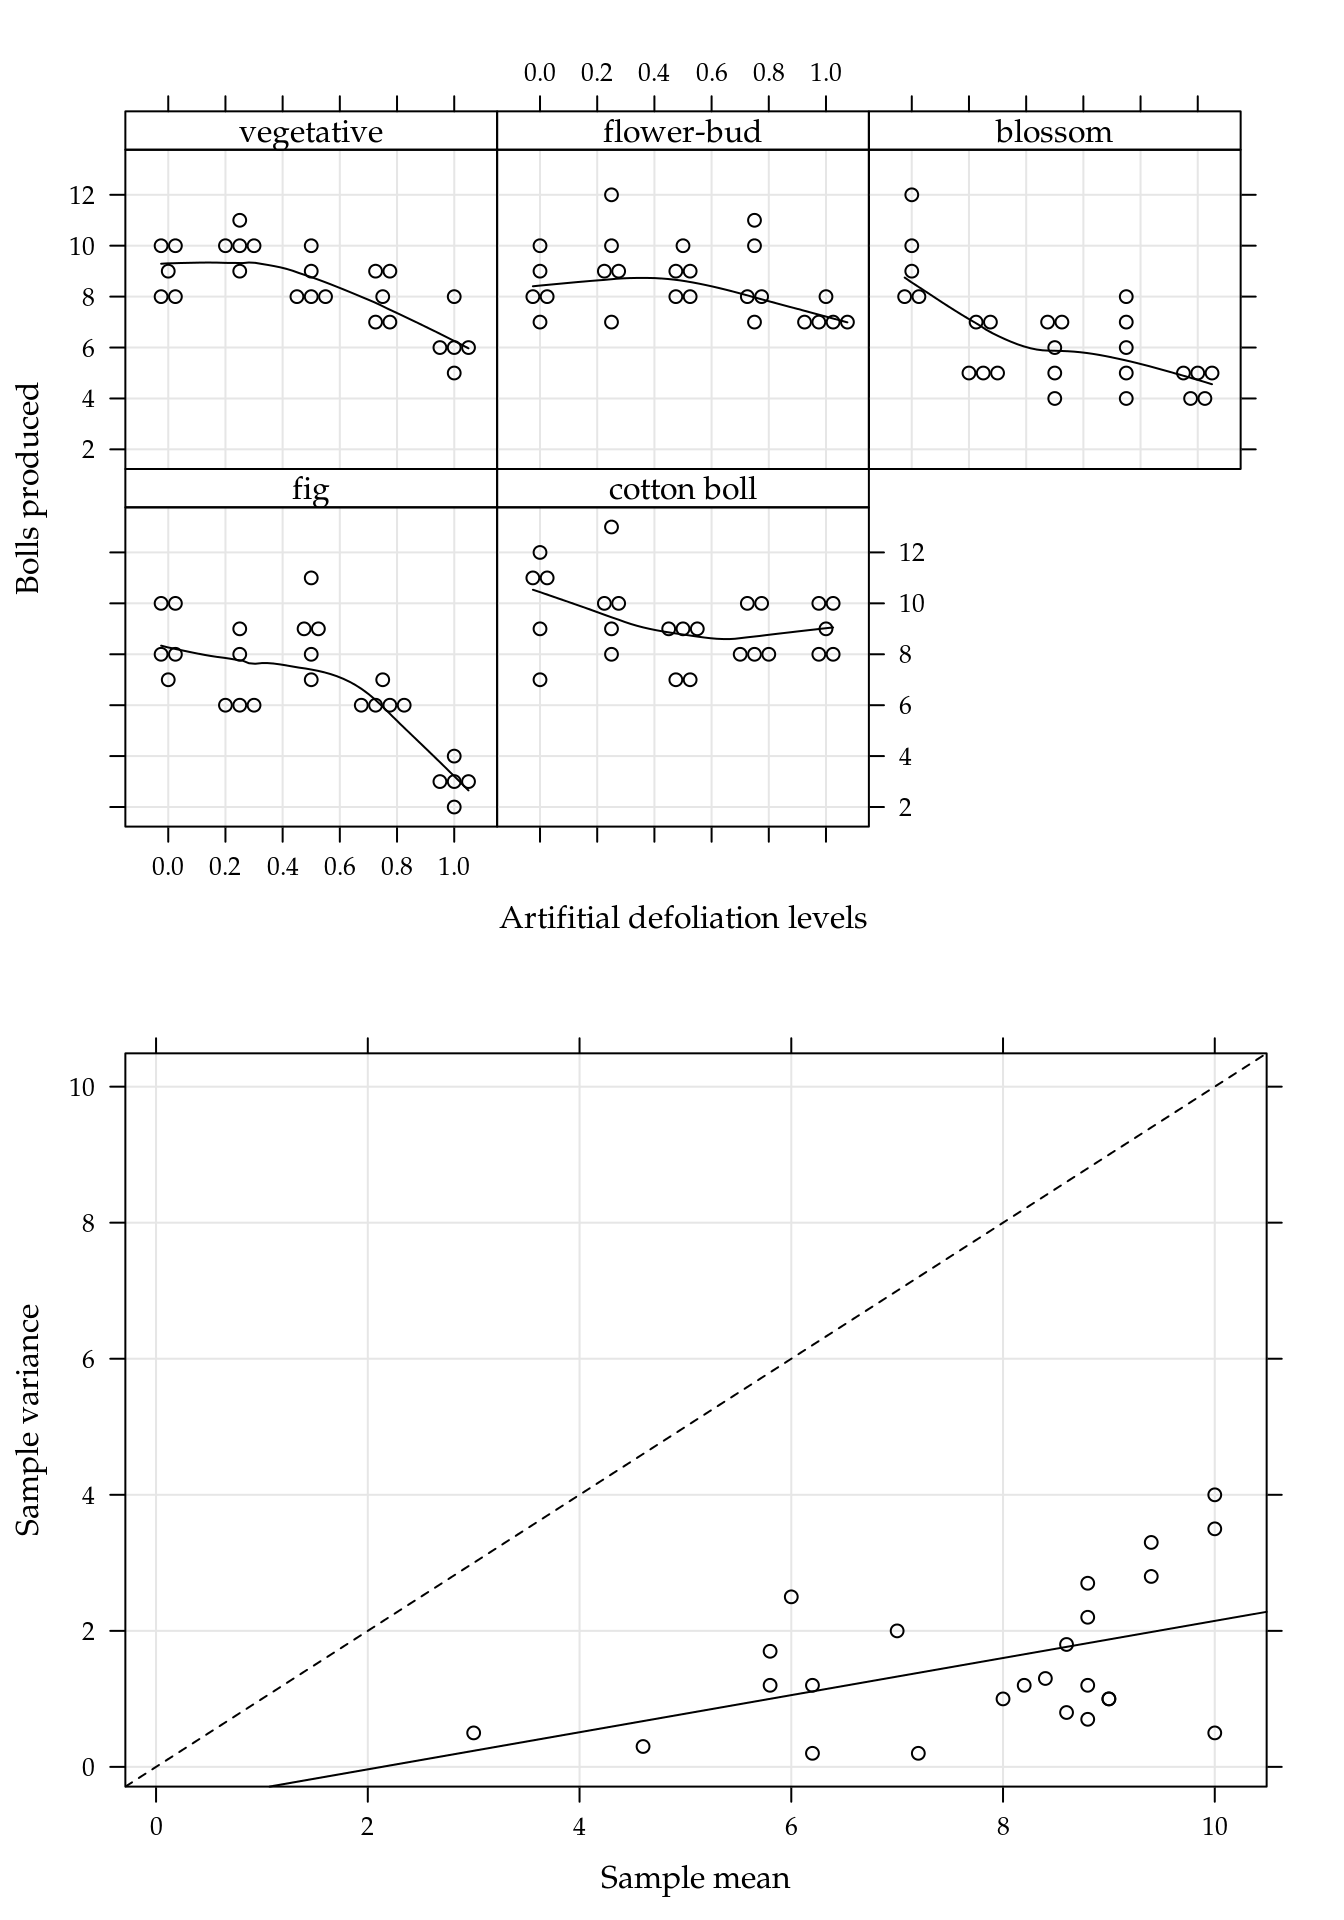
\includegraphics{rmcdbook_files/figure-latex/bools-mean-var-1} 

}

\caption{(top) Number of bolls produced for each artificial defoliation level and each growth stage. (bottom) Sample variance against the sample mean of the five replicates for each combination of defoliation level and growth stage.}\label{fig:bools-mean-var}
\end{figure}

The exploratory data analysis, although simple, was able to detect
departures from the Poisson equidispersion assumption. So, we have in
advance few conditions met for the use of GLM Poisson as a regression
model to analyse this experiment.

Poisson, as being a process derived from the memoryless waiting times
Exponential distribuition, implies that each boll is an independent
event in the artificial subjacent domain, that can be thought was the
natural resource domain that the plant has to allocate bolls. Its is
easy to assume, based on plant fisiology, that the probability of a boll
decreases with the number of previous bolls because the plant's resource
to produce bolls is limited and it is a non memoryless process
equivalent.

Based on the exploratory data analysis, a predictor with 2nd order
effect of defoliation for each growth stage should be enough to model
the number of bolls mean in a regression model. The analysis and
assessment of the effects of the experimental factors are based on the
Poisson, Gamma-count and Poisson Tweedie models.

\begin{Shaded}
\begin{Highlighting}[]
\NormalTok{m0 <-}\StringTok{ }\KeywordTok{glm}\NormalTok{(ncap ~}\StringTok{ }\NormalTok{est *}\StringTok{ }\NormalTok{(des +}\StringTok{ }\KeywordTok{I}\NormalTok{(des^}\DecValTok{2}\NormalTok{)),}
          \DataTypeTok{data =} \NormalTok{capdesfo,}
          \DataTypeTok{family =} \NormalTok{poisson)}

\KeywordTok{summary}\NormalTok{(m0)}
\end{Highlighting}
\end{Shaded}

\begin{verbatim}
## 
## Call:
## glm(formula = ncap ~ est * (des + I(des^2)), family = poisson, 
##     data = capdesfo)
## 
## Deviance Residuals: 
##     Min       1Q   Median       3Q      Max  
## -1.0771  -0.3098  -0.0228   0.2704   1.1665  
## 
## Coefficients:
##                         Estimate Std. Error z value Pr(>|z|)    
## (Intercept)               2.2142     0.1394   15.89   <2e-16 ***
## estflower-bud            -0.0800     0.2007   -0.40     0.69    
## estblossom               -0.0272     0.2001   -0.14     0.89    
## estfig                   -0.1486     0.2051   -0.72     0.47    
## estcotton boll            0.1129     0.1922    0.59     0.56    
## des                       0.3486     0.6805    0.51     0.61    
## I(des^2)                 -0.7384     0.6733   -1.10     0.27    
## estflower-bud:des         0.1364     0.9644    0.14     0.89    
## estblossom:des           -1.5819     1.0213   -1.55     0.12    
## estfig:des                0.4755     1.0194    0.47     0.64    
## estcotton boll:des       -0.8210     0.9395   -0.87     0.38    
## estflower-bud:I(des^2)    0.1044     0.9447    0.11     0.91    
## estblossom:I(des^2)       1.4044     1.0191    1.38     0.17    
## estfig:I(des^2)          -0.9294     1.0323   -0.90     0.37    
## estcotton boll:I(des^2)   1.0757     0.9210    1.17     0.24    
## ---
## Signif. codes:  0 '***' 0.001 '**' 0.01 '*' 0.05 '.' 0.1 ' ' 1
## 
## (Dispersion parameter for poisson family taken to be 1)
## 
##     Null deviance: 75.514  on 124  degrees of freedom
## Residual deviance: 25.331  on 110  degrees of freedom
## AIC: 539.7
## 
## Number of Fisher Scoring iterations: 4
\end{verbatim}

\begin{Shaded}
\begin{Highlighting}[]
\KeywordTok{logLik}\NormalTok{(m0)}
\end{Highlighting}
\end{Shaded}

\begin{verbatim}
## 'log Lik.' -255 (df=15)
\end{verbatim}

We fit the GLM Poisson regression model using the stardard
\texttt{glm()} function in R. The fitted model summary shows the
estimated parameters for the second order effect of defoliation crossed
with growth stages levels. The residual deviance was 25.33 based on 110
degrees of freedoom. The ratio \(25.33/110 = 0.23\) is a strong evidence
against Poisson equidispersion assumption that uses a dispersion
parameter equals 1.

\begin{Shaded}
\begin{Highlighting}[]
\KeywordTok{anova}\NormalTok{(m0, }\DataTypeTok{test =} \StringTok{"Chisq"}\NormalTok{)}
\end{Highlighting}
\end{Shaded}

\begin{verbatim}
## Analysis of Deviance Table
## 
## Model: poisson, link: log
## 
## Response: ncap
## 
## Terms added sequentially (first to last)
## 
## 
##              Df Deviance Resid. Df Resid. Dev Pr(>Chi)    
## NULL                           124       75.5             
## est           4    19.96       120       55.6  0.00051 ***
## des           1    15.86       119       39.7  6.8e-05 ***
## I(des^2)      1     1.29       118       38.4  0.25557    
## est:des       4     6.71       114       31.7  0.15212    
## est:I(des^2)  4     6.36       110       25.3  0.17388    
## ---
## Signif. codes:  0 '***' 0.001 '**' 0.01 '*' 0.05 '.' 0.1 ' ' 1
\end{verbatim}

The analysis of deviance table did not stated effect of any
interactions, neither second order effect of defiliation. Although, all
these effects are noticeable in Figure \ref{bools-mean-var}.

\begin{figure}[h]

{\centering 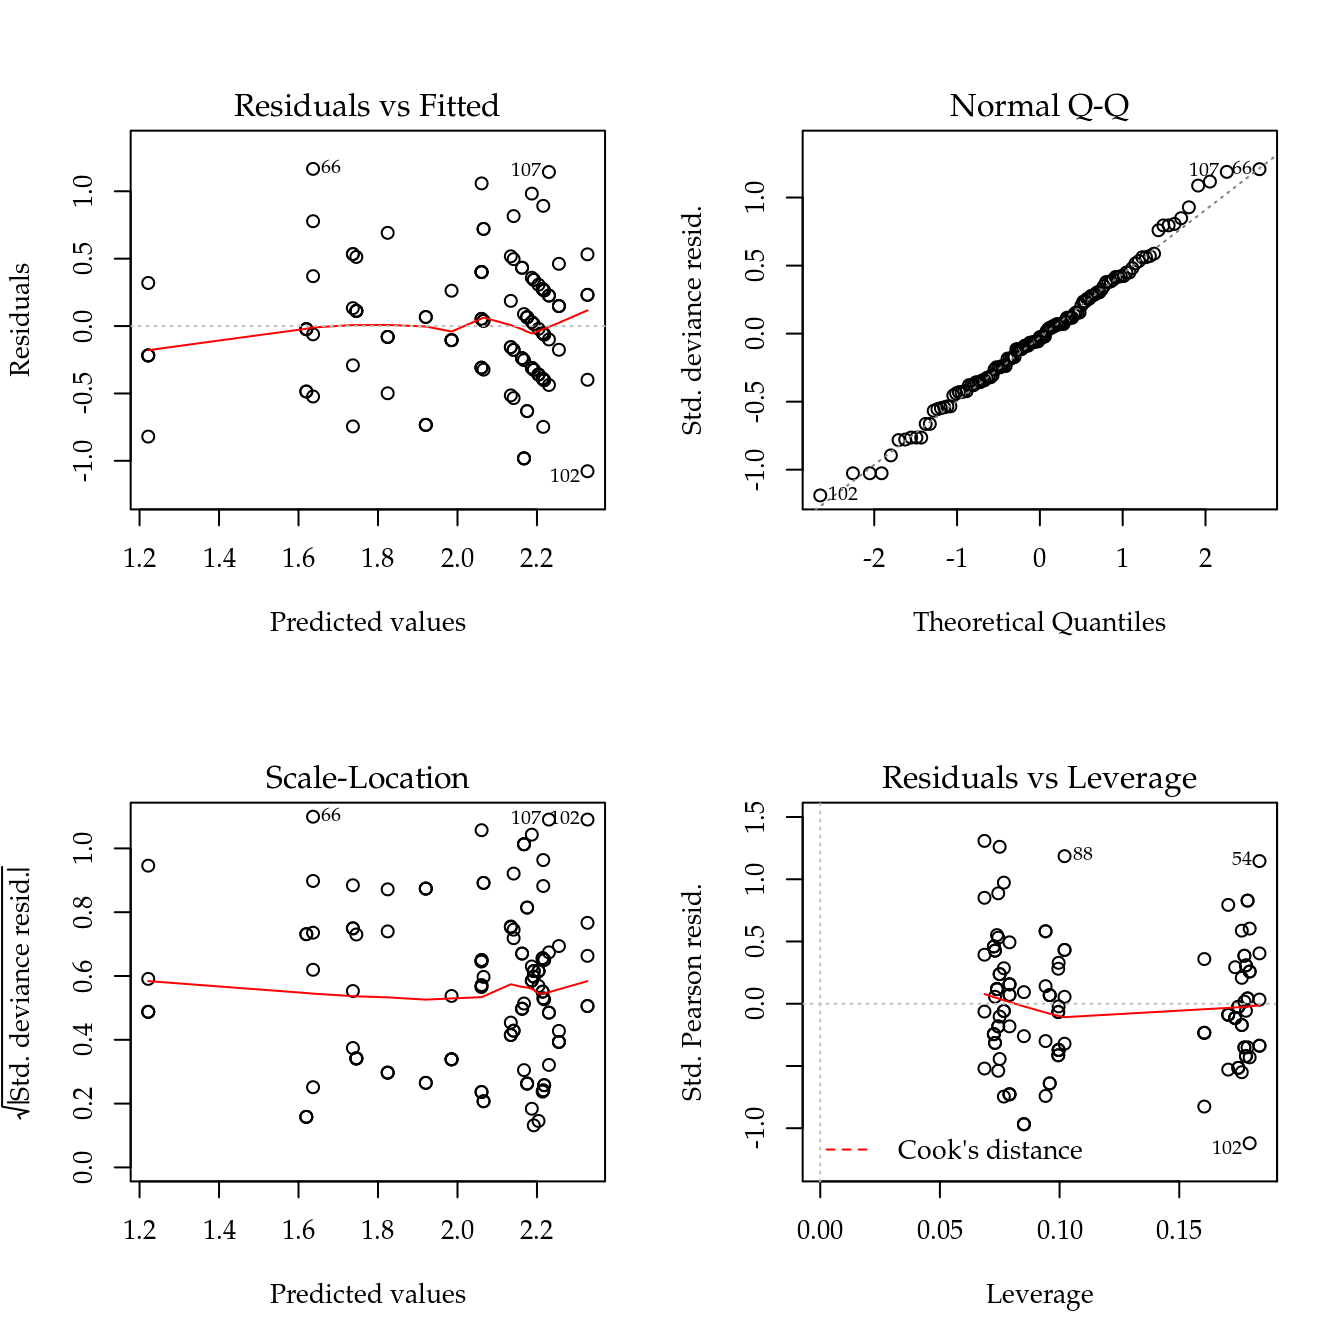
\includegraphics{rmcdbook_files/figure-latex/bolls-plot-residuals-1} 

}

\caption{The 4 plots for checking departures of assumptions in the GLM-Poisson regression model for the number of cotton bolls.}\label{fig:bolls-plot-residuals}
\end{figure}

Figure \ref{bolls-plot-residuals} displays the four residual plots for
the fitted model. Based on these plots, there is no concern about
mispecifications regarding to the model predictor or influential
observations. The only remarkable aspect is about the range of the
stardartized deviance residuals quite distant from the expected -3 to 3
from the normal distribution. Once more, these is another measure
indicating a underdispersed count data.

The \texttt{gcnt()} is a function defined in the \texttt{MRDCr} package
\citep{mrdcr-pkg} to fit the Gamma-Count regression model. This function
fits a GML-Poisson to use the estimates as initial values to optimize
Gamma-Count likelihood using \texttt{optim()} through \texttt{bblme}
package \citep{bblme-pkg}.

\begin{Shaded}
\begin{Highlighting}[]
\NormalTok{m1 <-}\StringTok{ }\KeywordTok{gcnt}\NormalTok{(ncap ~}\StringTok{ }\NormalTok{est *}\StringTok{ }\NormalTok{(des +}\StringTok{ }\KeywordTok{I}\NormalTok{(des^}\DecValTok{2}\NormalTok{)),}
           \DataTypeTok{data =} \NormalTok{capdesfo)}
\KeywordTok{summary}\NormalTok{(m1)}
\end{Highlighting}
\end{Shaded}

\begin{verbatim}
## Maximum likelihood estimation
## 
## Call:
## bbmle::mle2(minuslogl = llgcnt, start = start, data = list(y = y, 
##     X = X, offset = off), vecpar = TRUE)
## 
## Coefficients:
##                         Estimate Std. Error z value   Pr(z)    
## alpha                     1.7110     0.1352   12.66 < 2e-16 ***
## (Intercept)               2.2580     0.0593   38.05 < 2e-16 ***
## estflower-bud            -0.0765     0.0854   -0.90 0.37025    
## estblossom               -0.0253     0.0851   -0.30 0.76616    
## estfig                   -0.1398     0.0872   -1.60 0.10885    
## estcotton boll            0.1084     0.0818    1.33 0.18476    
## des                       0.3294     0.2896    1.14 0.25543    
## I(des^2)                 -0.6997     0.2866   -2.44 0.01464 *  
## estflower-bud:des         0.1337     0.4105    0.33 0.74456    
## estblossom:des           -1.5020     0.4345   -3.46 0.00055 ***
## estfig:des                0.4218     0.4336    0.97 0.33062    
## estcotton boll:des       -0.7820     0.3998   -1.96 0.05046 .  
## estflower-bud:I(des^2)    0.0943     0.4021    0.23 0.81452    
## estblossom:I(des^2)       1.3382     0.4335    3.09 0.00202 ** 
## estfig:I(des^2)          -0.8333     0.4390   -1.90 0.05768 .  
## estcotton boll:I(des^2)   1.0222     0.3920    2.61 0.00911 ** 
## ---
## Signif. codes:  0 '***' 0.001 '**' 0.01 '*' 0.05 '.' 0.1 ' ' 1
## 
## -2 log L: 408
\end{verbatim}

During the optimization process for this dataset, \texttt{optim()} has
found \texttt{NaN} when evaluating the likelihood. This occurs due
little numerical precision to calculate the difference of Gamma CDFs on
tails or for extreme values, resulting in numerical zeros and
corresponding \texttt{-Inf} log-likelihood. This is a numerical problem
that can narrow, or make things difficult, the use of Gamma-Count
regression model.

The dispersion parameter is the first position in the parameter vector.
The optimization was carried out on the log scale to avoid problems
regarding to bounded parameter spaces. As the dispersion parameter is in
fact interpreted as a precision coefficient, the positive estimate
indicates an underdispersed count. According to the \(z\) statistic,
\(\hat{alpha}\) is significantly different from zero (Poisson case).
Poisson is special case of Gamma-Count when \(\alpha = 0\), so we can
perform a likelihood ratio test to the hypothesis \(H_0: \alpha = 0\).

\begin{Shaded}
\begin{Highlighting}[]
\CommentTok{# Likelihood ratio test.}
\NormalTok{chi <-}\StringTok{ }\DecValTok{2} \NormalTok{*}\StringTok{ }\NormalTok{(}\KeywordTok{logLik}\NormalTok{(m1) -}\StringTok{ }\KeywordTok{logLik}\NormalTok{(m0))}
\NormalTok{pval <-}\StringTok{ }\DecValTok{2} \NormalTok{*}\StringTok{ }\KeywordTok{pchisq}\NormalTok{(chi, }\DataTypeTok{df =} \DecValTok{1}\NormalTok{, }\DataTypeTok{lower.tail =} \OtherTok{FALSE}\NormalTok{)}
\KeywordTok{cat}\NormalTok{(}\StringTok{"Likelihood Ratio Test}\CharTok{\textbackslash{}n}\StringTok{"}\NormalTok{,}
    \StringTok{"Chisq:}\CharTok{\textbackslash{}t\textbackslash{}t}\StringTok{ "}\NormalTok{, chi, }\StringTok{"}\CharTok{\textbackslash{}n}\StringTok{"}\NormalTok{,}
    \StringTok{"Pr(>Chisq):}\CharTok{\textbackslash{}t}\StringTok{ "}\NormalTok{, pval, }\StringTok{"}\CharTok{\textbackslash{}n}\StringTok{"}\NormalTok{,}
    \DataTypeTok{sep =} \StringTok{""}\NormalTok{)}
\end{Highlighting}
\end{Shaded}

\begin{verbatim}
## Likelihood Ratio Test
## Chisq:        102
## Pr(>Chisq):   1.01e-23
\end{verbatim}

\begin{Shaded}
\begin{Highlighting}[]
\CommentTok{# Log-likelihood profile for alpha.}
\KeywordTok{plot}\NormalTok{(}\KeywordTok{profile}\NormalTok{(m1, }\DataTypeTok{which =} \StringTok{"alpha"}\NormalTok{))}
\end{Highlighting}
\end{Shaded}

\begin{center}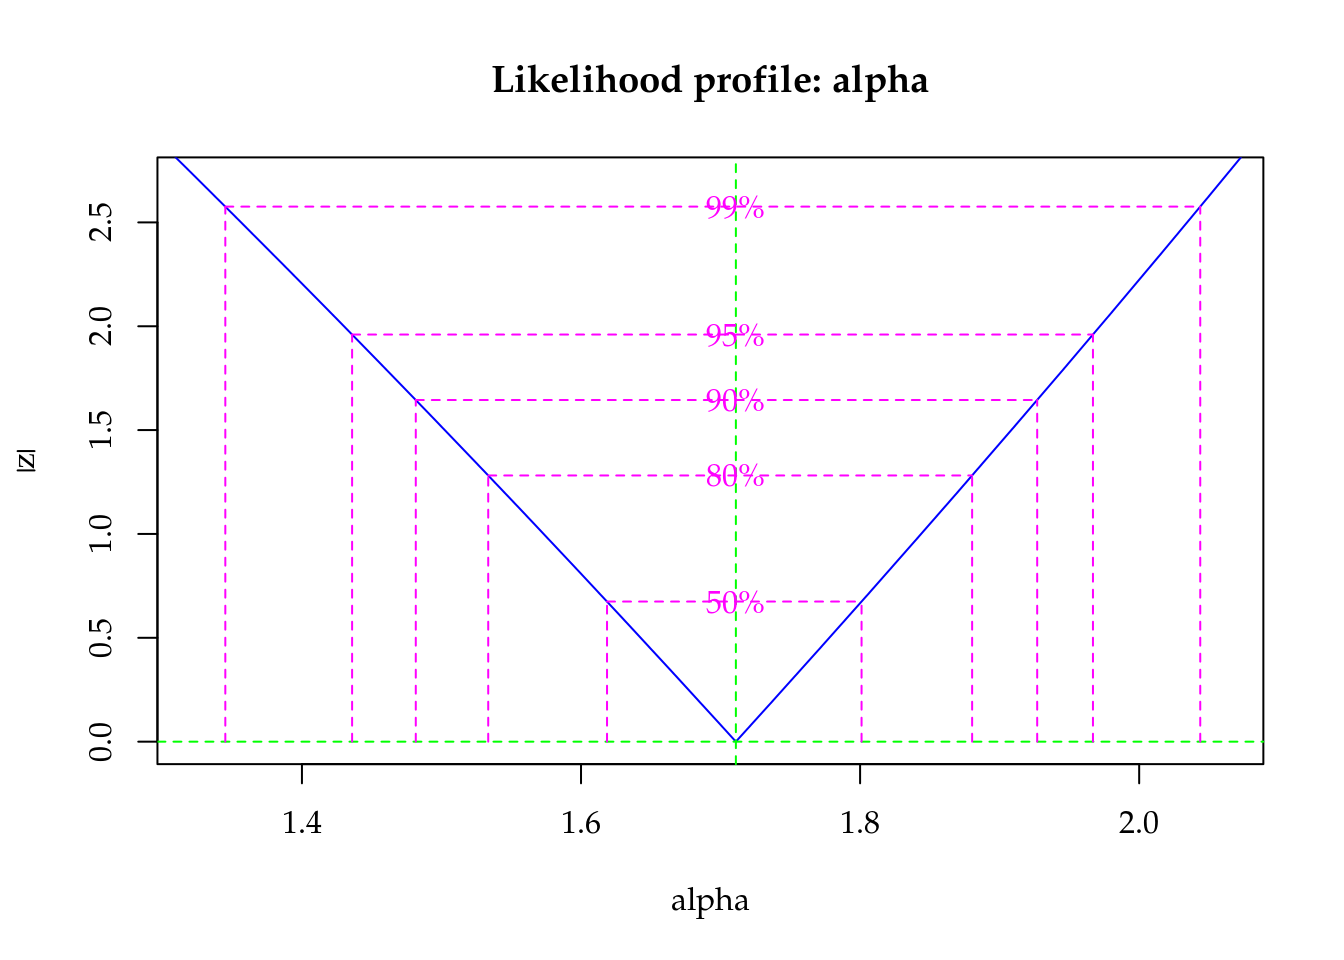
\includegraphics{rmcdbook_files/figure-latex/unnamed-chunk-15-1} \end{center}

\begin{Shaded}
\begin{Highlighting}[]
\KeywordTok{cbind}\NormalTok{(}\KeywordTok{c}\NormalTok{(}\DecValTok{0}\NormalTok{, }\KeywordTok{coef}\NormalTok{(m0)), }\KeywordTok{coef}\NormalTok{(m1))}
\end{Highlighting}
\end{Shaded}

\begin{verbatim}
##                            [,1]    [,2]
##                          0.0000  1.7110
## (Intercept)              2.2142  2.2580
## estflower-bud           -0.0800 -0.0765
## estblossom              -0.0272 -0.0253
## estfig                  -0.1486 -0.1398
## estcotton boll           0.1129  0.1084
## des                      0.3486  0.3294
## I(des^2)                -0.7384 -0.6997
## estflower-bud:des        0.1364  0.1337
## estblossom:des          -1.5819 -1.5020
## estfig:des               0.4755  0.4218
## estcotton boll:des      -0.8210 -0.7820
## estflower-bud:I(des^2)   0.1044  0.0943
## estblossom:I(des^2)      1.4044  1.3382
## estfig:I(des^2)         -0.9294 -0.8333
## estcotton boll:I(des^2)  1.0757  1.0222
\end{verbatim}

\begin{Shaded}
\begin{Highlighting}[]
\NormalTok{rstd <-}\StringTok{ }\KeywordTok{summary}\NormalTok{(m1)@coef[-}\DecValTok{1}\NormalTok{, }\DecValTok{2}\NormalTok{]/}\KeywordTok{summary}\NormalTok{(m0)$coeff[, }\DecValTok{2}\NormalTok{]}
\NormalTok{plyr::}\KeywordTok{each}\NormalTok{(mean, range)(rstd)}
\end{Highlighting}
\end{Shaded}

\begin{verbatim}
##   mean range1 range2 
##  0.426  0.425  0.426
\end{verbatim}

The estimates for the location parameters were very close. The ratio
between Gamma-Count parameters standard error and Poisson ones, on the
other hand, were 0.426 for all estimates, for 3 decimals of precision.
This leads to the conclusion that TODO relação linear no parâmetro de
dispersão.

\begin{Shaded}
\begin{Highlighting}[]
\CommentTok{# Wald test for the interaction.}
\NormalTok{a <-}\StringTok{ }\KeywordTok{c}\NormalTok{(}\DecValTok{0}\NormalTok{, }\KeywordTok{attr}\NormalTok{(}\KeywordTok{model.matrix}\NormalTok{(m0), }\StringTok{"assign"}\NormalTok{))}
\NormalTok{ai <-}\StringTok{ }\NormalTok{a ==}\StringTok{ }\KeywordTok{max}\NormalTok{(a)}
\NormalTok{L <-}\StringTok{ }\KeywordTok{t}\NormalTok{(}\KeywordTok{replicate}\NormalTok{(}\KeywordTok{sum}\NormalTok{(ai), }\KeywordTok{rbind}\NormalTok{(}\KeywordTok{coef}\NormalTok{(m1) *}\StringTok{ }\DecValTok{0}\NormalTok{), }\DataTypeTok{simplify =} \StringTok{"matrix"}\NormalTok{))}
\NormalTok{L[, ai] <-}\StringTok{ }\KeywordTok{diag}\NormalTok{(}\KeywordTok{sum}\NormalTok{(ai))}

\KeywordTok{linearHypothesis}\NormalTok{(}\DataTypeTok{model =} \NormalTok{m0, }\CommentTok{# m0 is not being used here.}
                 \DataTypeTok{hypothesis.matrix =} \NormalTok{L,}
                 \DataTypeTok{vcov. =} \KeywordTok{vcov}\NormalTok{(m1),}
                 \DataTypeTok{coef. =} \KeywordTok{coef}\NormalTok{(m1))}
\end{Highlighting}
\end{Shaded}

\begin{verbatim}
## Linear hypothesis test
## 
## Hypothesis:
## estflower - bud:I(des^2) = 0
## estblossom:I(des^2) = 0
## estfig:I(des^2) = 0
## estcotton boll:I(des^2) = 0
## 
## Model 1: restricted model
## Model 2: ncap ~ est * (des + I(des^2))
## 
## Note: Coefficient covariance matrix supplied.
## 
##   Res.Df Df Chisq Pr(>Chisq)    
## 1    114                        
## 2    110  4  30.5    3.8e-06 ***
## ---
## Signif. codes:  0 '***' 0.001 '**' 0.01 '*' 0.05 '.' 0.1 ' ' 1
\end{verbatim}

\begin{Shaded}
\begin{Highlighting}[]
\CommentTok{# Fitting Poisson-Tweedie model.}
\NormalTok{m2 <-}\StringTok{ }\KeywordTok{mcglm}\NormalTok{(}\DataTypeTok{linear_pred =} \KeywordTok{c}\NormalTok{(ncap ~}\StringTok{ }\NormalTok{est *}\StringTok{ }\NormalTok{(des +}\StringTok{ }\KeywordTok{I}\NormalTok{(des^}\DecValTok{2}\NormalTok{))),}
            \DataTypeTok{matrix_pred =} \KeywordTok{list}\NormalTok{(}\KeywordTok{mc_id}\NormalTok{(}\DataTypeTok{data =} \NormalTok{capdesfo)),}
            \DataTypeTok{link =} \StringTok{"log"}\NormalTok{,}
            \DataTypeTok{variance =} \StringTok{"poisson_tweedie"}\NormalTok{,}
            \DataTypeTok{power_fixed =} \OtherTok{FALSE}\NormalTok{,}
            \DataTypeTok{data =} \NormalTok{capdesfo,}
            \DataTypeTok{control_algorithm =} \KeywordTok{list}\NormalTok{(}\DataTypeTok{verbose =} \OtherTok{FALSE}\NormalTok{,}
                                     \DataTypeTok{max_iter =} \DecValTok{100}\NormalTok{,}
                                     \DataTypeTok{tunning =} \FloatTok{0.5}\NormalTok{,}
                                     \DataTypeTok{correct =} \OtherTok{FALSE}\NormalTok{))}
\end{Highlighting}
\end{Shaded}

\begin{verbatim}
## Automatic initial values selected.
\end{verbatim}

\begin{Shaded}
\begin{Highlighting}[]
\CommentTok{# Parameter estimates.}
\KeywordTok{summary}\NormalTok{(m2)}
\end{Highlighting}
\end{Shaded}

\begin{verbatim}
## Call: ncap ~ est * (des + I(des^2))
## 
## Link function: log
## Variance function: poisson_tweedie
## Covariance function: identity
## Regression:
##                         Estimates Std.error Z value
## (Intercept)                2.2143    0.0627  35.308
## estflower-bud             -0.0800    0.0904  -0.886
## estblossom                -0.0265    0.0900  -0.294
## estfig                    -0.1485    0.0924  -1.607
## estcotton boll             0.1128    0.0864   1.306
## des                        0.3486    0.3065   1.137
## I(des^2)                  -0.7385    0.3037  -2.432
## estflower-bud:des          0.1361    0.4345   0.313
## estblossom:des            -1.5875    0.4612  -3.442
## estfig:des                 0.4693    0.4602   1.020
## estcotton boll:des        -0.8204    0.4228  -1.940
## estflower-bud:I(des^2)     0.1048    0.4259   0.246
## estblossom:I(des^2)        1.4098    0.4609   3.059
## estfig:I(des^2)           -0.9205    0.4671  -1.971
## estcotton boll:I(des^2)    1.0752    0.4149   2.592
## 
## Power:
##   Estimates Std.error Z value
## 1      1.01     0.136    7.43
## 
## Dispersion:
##   Estimates Std.error Z value
## 1    -0.781     0.217   -3.59
## 
## Algorithm: chaser
## Correction: FALSE
## Number iterations: 14
\end{verbatim}

\begin{Shaded}
\begin{Highlighting}[]
\KeywordTok{plot}\NormalTok{(m2, }\DataTypeTok{type =} \StringTok{"algorithm"}\NormalTok{)}
\end{Highlighting}
\end{Shaded}

\begin{center}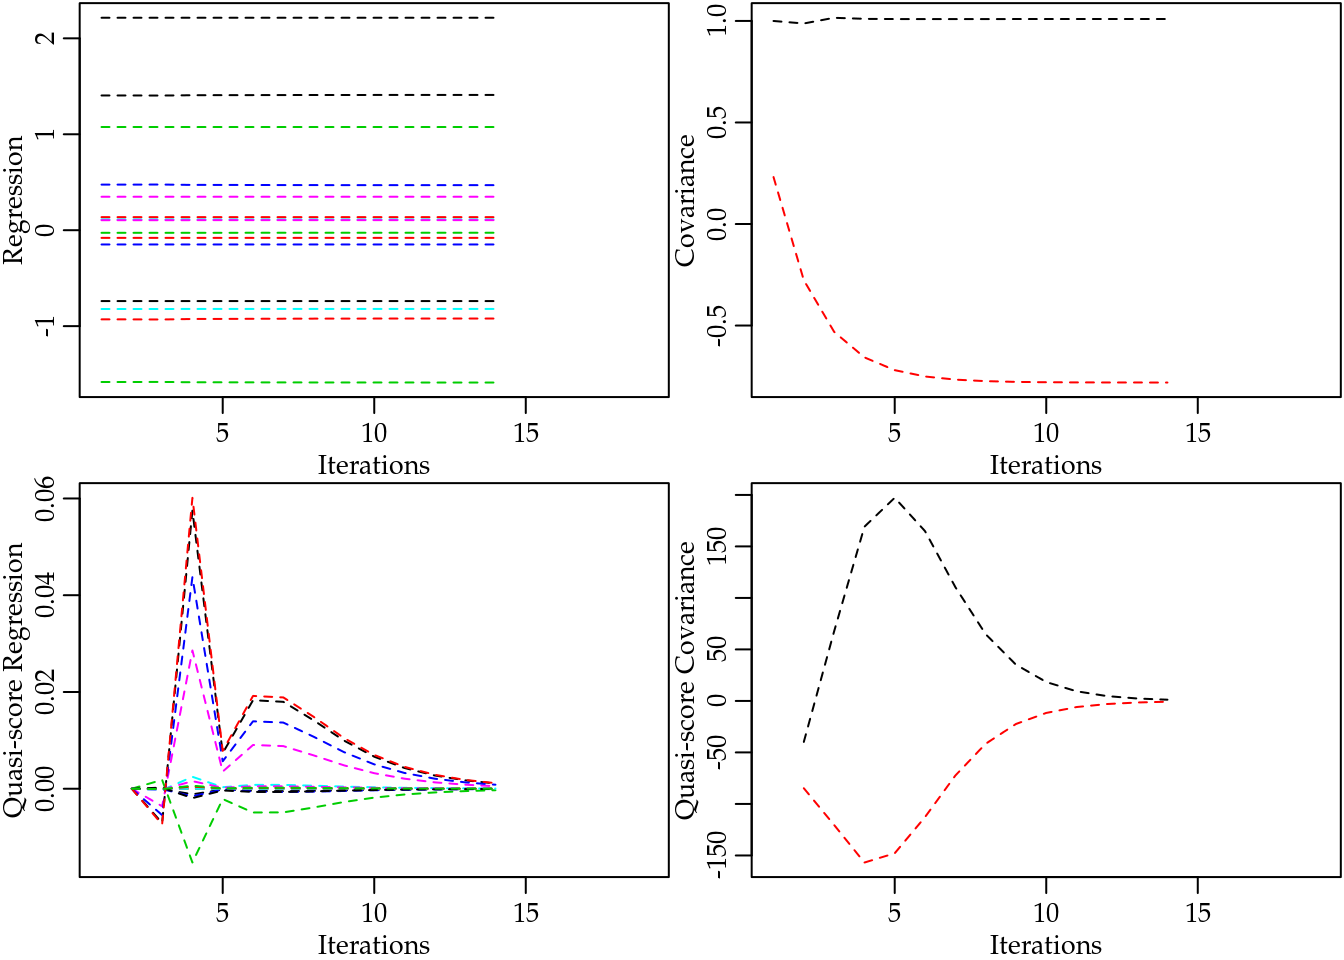
\includegraphics{rmcdbook_files/figure-latex/unnamed-chunk-18-1} \end{center}

\begin{Shaded}
\begin{Highlighting}[]
\CommentTok{# Wald test for fixed effects.}
\KeywordTok{anova}\NormalTok{(m2)}
\end{Highlighting}
\end{Shaded}

\begin{verbatim}
## Wald test for fixed effects
## Call: ncap ~ est * (des + I(des^2))
## 
##                Covariate Chi.Square Df p.value
## 1          estflower-bud       9.54  4  0.0489
## 2                    des       1.29  1  0.2555
## 3               I(des^2)       5.91  1  0.0150
## 4      estflower-bud:des      25.00  4  0.0001
## 5 estflower-bud:I(des^2)      30.72  4  0.0000
\end{verbatim}

\begin{Shaded}
\begin{Highlighting}[]
\CommentTok{# New data values for prediction.}
\NormalTok{pred <-}\StringTok{ }\KeywordTok{with}\NormalTok{(capdesfo,}
             \KeywordTok{expand.grid}\NormalTok{(}\DataTypeTok{est =} \KeywordTok{levels}\NormalTok{(est),}
                         \DataTypeTok{des =} \KeywordTok{seq}\NormalTok{(}\DecValTok{0}\NormalTok{, }\DecValTok{1}\NormalTok{, }\DataTypeTok{length.out =} \DecValTok{30}\NormalTok{)))}

\CommentTok{# Corresponding model matrix.}
\NormalTok{X <-}\StringTok{ }\KeywordTok{model.matrix}\NormalTok{(}\KeywordTok{formula}\NormalTok{(m0)[-}\DecValTok{2}\NormalTok{], }\DataTypeTok{data =} \NormalTok{pred)}

\CommentTok{#--------------------------------------------}
\CommentTok{# Poisson.}

\NormalTok{yp <-}\StringTok{ }\KeywordTok{predict}\NormalTok{(m0, }\DataTypeTok{newdata =} \NormalTok{pred, }\DataTypeTok{se.fit =} \OtherTok{TRUE}\NormalTok{)}
\NormalTok{em <-}\StringTok{ }\KeywordTok{outer}\NormalTok{(yp$se.fit,}
            \KeywordTok{c}\NormalTok{(}\DataTypeTok{lwrP =} \NormalTok{-}\DecValTok{1}\NormalTok{, }\DataTypeTok{fitP =} \DecValTok{0}\NormalTok{, }\DataTypeTok{uprP =} \DecValTok{1}\NormalTok{) *}\StringTok{ }\KeywordTok{qnorm}\NormalTok{(}\FloatTok{0.975}\NormalTok{),}
            \DataTypeTok{FUN =} \StringTok{"*"}\NormalTok{)}
\NormalTok{ci <-}\StringTok{ }\KeywordTok{sweep}\NormalTok{(em, }\DataTypeTok{MARGIN =} \DecValTok{1}\NormalTok{, }\DataTypeTok{STATS =} \NormalTok{yp$fit, }\DataTypeTok{FUN =} \StringTok{"+"}\NormalTok{)}
\NormalTok{ci <-}\StringTok{ }\NormalTok{m0$family$}\KeywordTok{linkinv}\NormalTok{(ci)}

\NormalTok{pred <-}\StringTok{ }\KeywordTok{cbind}\NormalTok{(pred, }\KeywordTok{as.data.frame}\NormalTok{(ci))}
\KeywordTok{str}\NormalTok{(pred)}
\end{Highlighting}
\end{Shaded}

\begin{verbatim}
## 'data.frame':    150 obs. of  5 variables:
##  $ est : Factor w/ 5 levels "vegetative","flower-bud",..: 1 2 3 4 5 1 2 3 4 5 ...
##  $ des : num  0 0 0 0 0 ...
##  $ lwrP: num  6.97 6.37 6.72 5.88 7.91 ...
##  $ fitP: num  9.15 8.45 8.91 7.89 10.25 ...
##  $ uprP: num  12 11.2 11.8 10.6 13.3 ...
\end{verbatim}

\begin{Shaded}
\begin{Highlighting}[]
\CommentTok{# TODO predito pelo 3 modelos.}
\end{Highlighting}
\end{Shaded}

TODO: pares de estimativa e erros padrões.

\section{Soybean pod and beans}\label{soybean-pod-and-beans}

The tropical soils, usually poor in potassium (K), demand potassium
fertilization when cultivated with soybean (\emph{Glycine max} L.) to
obtain satisfactory yields. Soybean production is affected by long
exposition to water deficit. As postassium is a nutrient involved in the
water balance in plant, by hyphotesis, a good supply of potassium avoids
lose production.

The aim of this experiment was to evaluate the effects of K doses and
soil humidity levels on soybean production. The experiment was carried
out in a greenhouse, in pots with two plants, containing 5
dm\textsuperscript{3} of soil. The experimental design was completely
randomized block with treatments in a 5 x 3 factorial arrangement. The K
doses were 0, 30, 60, 120 and 180 mg dm\textsuperscript{-3} , and the
soil humidity ranged from 35 to 40, 47.5 to 52.5, and 60 to 65\% of the
total porosity \citep[for more details]{Serafim2012}.

Two count variables were recorded in this experiment: the total number
of pods per plot and the total number of grains per plot. The ratio,
grains/pod, can also be analysed, since the fisiological response can
change it.

There is an outlier in the dataset at position 74 that must be removed.
Potassion amount (K) will be converted to a categorical factor, despite
it is a numerical one, to prevent concerns with lack of fit, that is not
the main scope of the following analysis.

\begin{Shaded}
\begin{Highlighting}[]
\KeywordTok{data}\NormalTok{(soja)}
\KeywordTok{str}\NormalTok{(soja)}
\end{Highlighting}
\end{Shaded}

\begin{verbatim}
## 'data.frame':    75 obs. of  5 variables:
##  $ K   : int  0 30 60 120 180 0 30 60 120 180 ...
##  $ umid: Factor w/ 3 levels "37,5","50","62,5": 1 1 1 1 1 2 2 2 2 2 ...
##  $ bloc: Factor w/ 5 levels "I","II","III",..: 1 1 1 1 1 1 1 1 1 1 ...
##  $ ngra: int  136 159 156 171 190 140 193 200 208 237 ...
##  $ nvag: int  56 62 66 68 82 63 86 94 86 97 ...
\end{verbatim}

\begin{Shaded}
\begin{Highlighting}[]
\CommentTok{# Removing an outlier.}
\NormalTok{soja <-}\StringTok{ }\NormalTok{soja[-}\DecValTok{74}\NormalTok{, ]}
\NormalTok{soja <-}\StringTok{ }\KeywordTok{transform}\NormalTok{(soja, }\DataTypeTok{K =} \KeywordTok{factor}\NormalTok{(K))}
\end{Highlighting}
\end{Shaded}

\subsection{Number of pods}\label{number-of-pods}

The pod is a dehiscent fruit of a leguminous plant such as the beans and
soybeans. The pod is the basic unit of production in soybean, so factors
that reduces or increases the number of pods have impact in crop
production.

The potassium amount (K) increased the number of pods and number of
beans in all soil water content levels (A)
(\ref{fig:pods-beans-scatter}). For lowest soil water level, the mean
was fairly low than the other levels that perform very similar. The
pattern driven by the mean lines suggests interaction between applied
potassium amount and soil water content for both variables.

We could obtain the sample variance and sample mean for each cell
combination for checking dispersion level but it would ignore the block
effect, that can enlarges the variance.

\begin{Shaded}
\begin{Highlighting}[]
\KeywordTok{xyplot}\NormalTok{(nvag +}\StringTok{ }\NormalTok{ngra ~}\StringTok{ }\NormalTok{K,}
       \DataTypeTok{groups =} \NormalTok{umid,}
       \DataTypeTok{outer =} \OtherTok{TRUE}\NormalTok{,}
       \DataTypeTok{data =} \NormalTok{soja,}
       \DataTypeTok{type =} \KeywordTok{c}\NormalTok{(}\StringTok{"p"}\NormalTok{, }\StringTok{"a"}\NormalTok{),}
       \DataTypeTok{scales =} \StringTok{"free"}\NormalTok{,}
       \DataTypeTok{ylab =} \OtherTok{NULL}\NormalTok{,}
       \DataTypeTok{xlab =} \KeywordTok{expression}\NormalTok{(}\StringTok{"Applied potassium amount"} \NormalTok{~}\StringTok{ }\NormalTok{(mg ~}\StringTok{ }\NormalTok{dm^\{-}\DecValTok{3}\NormalTok{\})),}
       \DataTypeTok{auto.key =} \KeywordTok{list}\NormalTok{(}\DataTypeTok{title =} \StringTok{"Soil water content (%)"}\NormalTok{,}
                       \DataTypeTok{cex.title =} \DecValTok{1}\NormalTok{,}
                       \DataTypeTok{columns =} \DecValTok{3}\NormalTok{),}
       \DataTypeTok{strip =} \KeywordTok{strip.custom}\NormalTok{(}
           \DataTypeTok{factor.levels =} \KeywordTok{c}\NormalTok{(}\StringTok{"Number of pods"}\NormalTok{,}
                             \StringTok{"Number of beans"}\NormalTok{)))}
\end{Highlighting}
\end{Shaded}

\textbackslash{}begin\{figure\}{[}h{]}

\{\centering 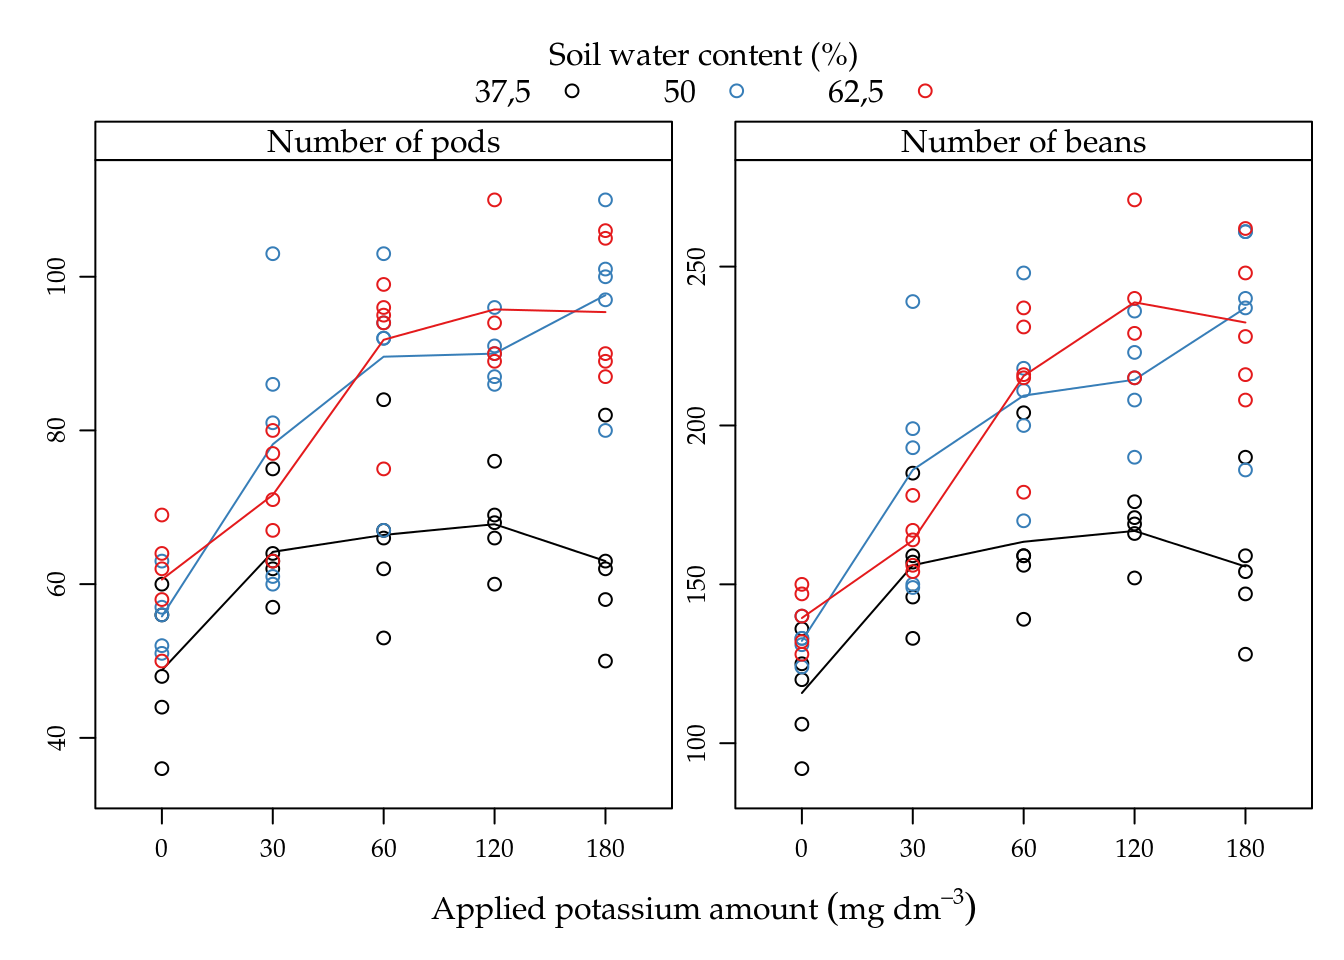
\includegraphics{rmcdbook_files/figure-latex/pods-beans-scatter-1}

\}

\textbackslash{}caption\{Number of pods and beans as function of
potassium amount (K) for each soil water content level (\%). Lines
passes on the average of points. The mean response pattern is the same
on the two variables.\}\label{fig:pods-beans-scatter}
\textbackslash{}end\{figure\}

The following analysis with be carried out in parallel, that is, results
will be showed together in each step for the sake of comparison.

We fit Poisson (P), Gamma-Count (GC) and Poisson-Tweedie (TW) regression
models. The first two were fit by maximum likelihood and the last by
moments specification.

\begin{Shaded}
\begin{Highlighting}[]
\CommentTok{#--------------------------------------------}
\CommentTok{# Poisson.}

\NormalTok{m0 <-}\StringTok{ }\KeywordTok{glm}\NormalTok{(nvag ~}\StringTok{ }\NormalTok{bloc +}\StringTok{ }\NormalTok{umid *}\StringTok{ }\NormalTok{K,}
          \DataTypeTok{data =} \NormalTok{soja,}
          \DataTypeTok{family =} \NormalTok{poisson)}

\CommentTok{#--------------------------------------------}
\CommentTok{# Gamma-Count.}

\NormalTok{m1 <-}\StringTok{ }\KeywordTok{gcnt}\NormalTok{(}\KeywordTok{formula}\NormalTok{(m0), }\DataTypeTok{data =} \NormalTok{soja)}

\CommentTok{#--------------------------------------------}
\CommentTok{# Tweedie.}

\NormalTok{m2 <-}\StringTok{ }\KeywordTok{mcglm}\NormalTok{(}\DataTypeTok{linear_pred =} \KeywordTok{c}\NormalTok{(nvag ~}\StringTok{ }\NormalTok{bloc +}\StringTok{ }\NormalTok{umid *}\StringTok{ }\NormalTok{K),}
            \DataTypeTok{matrix_pred =} \KeywordTok{list}\NormalTok{(}\KeywordTok{mc_id}\NormalTok{(}\DataTypeTok{data =} \NormalTok{soja)),}
            \DataTypeTok{link =} \StringTok{"log"}\NormalTok{,}
            \DataTypeTok{variance =} \StringTok{"poisson_tweedie"}\NormalTok{,}
            \DataTypeTok{power_fixed =} \OtherTok{TRUE}\NormalTok{,}
            \DataTypeTok{data =} \NormalTok{soja,}
            \DataTypeTok{control_algorithm =} \KeywordTok{list}\NormalTok{(}\DataTypeTok{verbose =} \OtherTok{FALSE}\NormalTok{,}
                                     \DataTypeTok{max_iter =} \DecValTok{100}\NormalTok{,}
                                     \DataTypeTok{tunning =} \FloatTok{0.5}\NormalTok{,}
                                     \DataTypeTok{correct =} \OtherTok{FALSE}\NormalTok{))}
\end{Highlighting}
\end{Shaded}

\begin{verbatim}
## Automatic initial values selected.
\end{verbatim}

To fit Poisson and Gamma-Count, the correspond function were used in the
default setting. To fit Poisson Tweedie, we
\texttt{power\_fixed\ =\ TRUE} option, since the number of pods is a
close to equidispersed count variable. The Poisson-Tweedie loses
identifiability in the equidispersion zone because the variance is
\(var(Y) = \mu + \phi\mu^p\), then \(p\) can be any value if \(\phi\)
goes to zero. We fixed \(p = 1\).

\begin{figure}[h]

{\centering 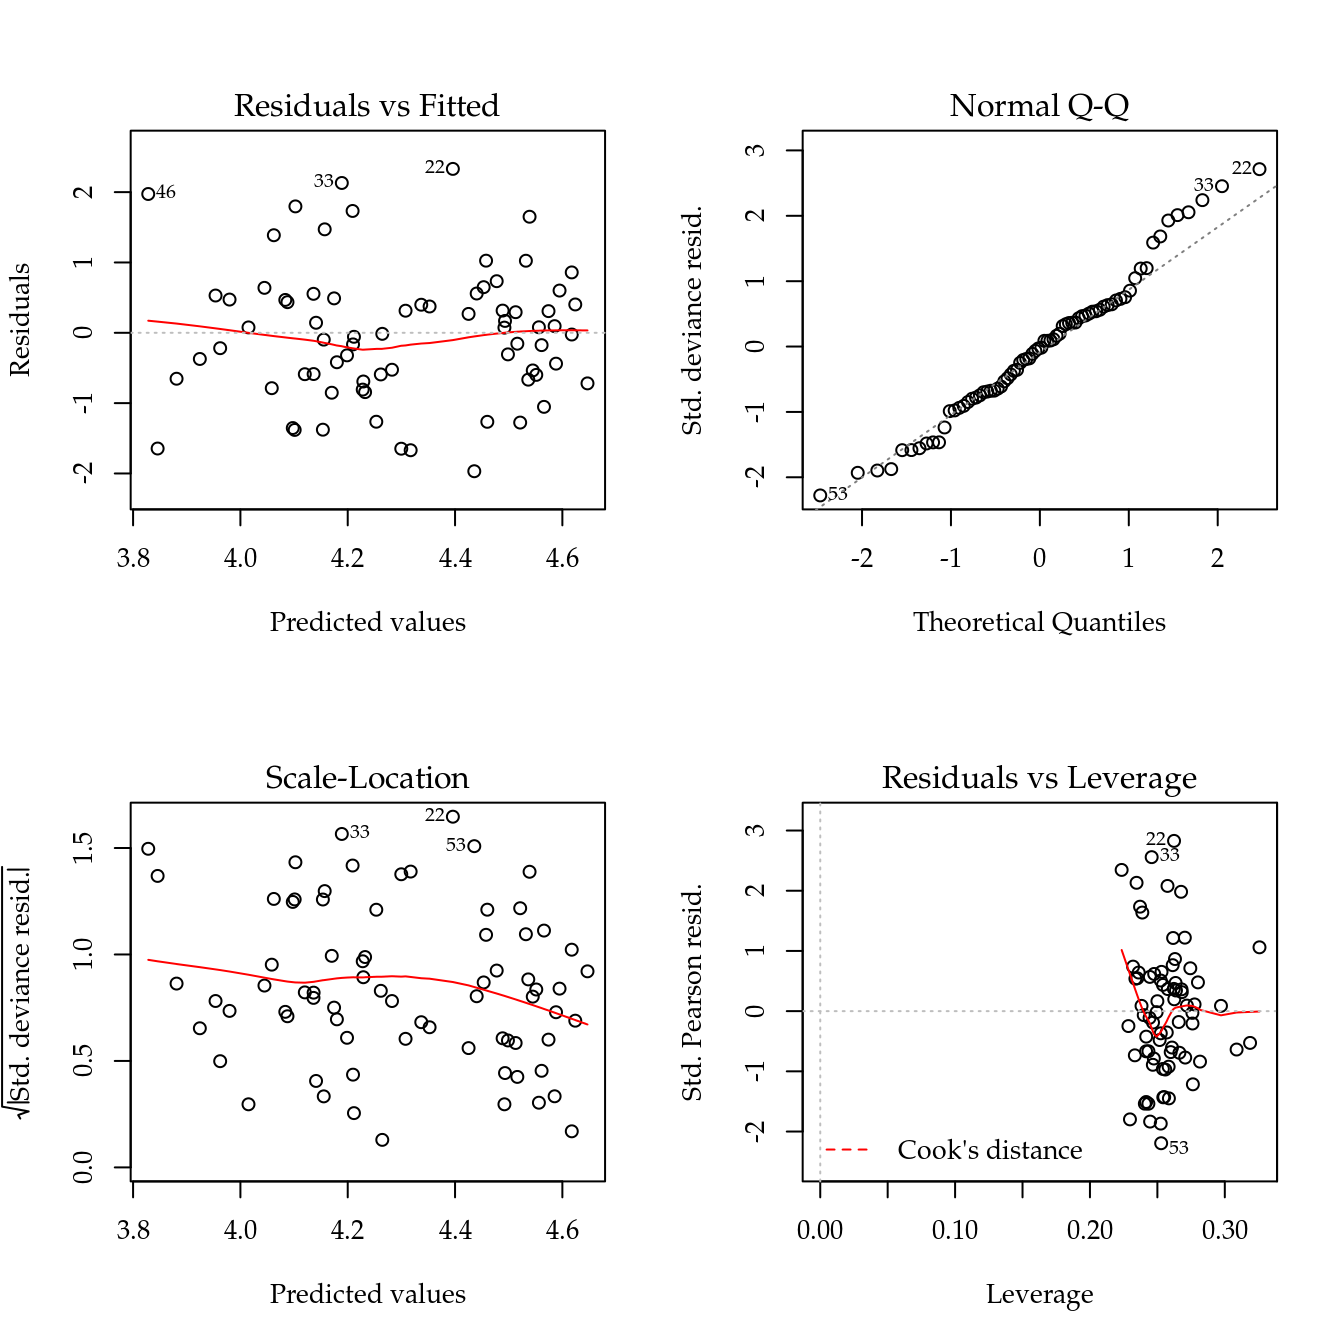
\includegraphics{rmcdbook_files/figure-latex/pods-plot-residuals-1} 

}

\caption{The 4 plots for checking departures of assumptions in the GLM-Poisson regression model for number of soybean pods.}\label{fig:pods-plot-residuals}
\end{figure}

Figure \ref{fig:pods-plot-residuals} shows the 4 plots based on
residuals. This residuals didn't show any departure pattern. On the
contray, the axes of the qq-norm plot shows the same range, indicating a
equidispersed count variable.

The maximised log-likelihood were very close for Poisson and Gamma-Count
models. The profile log-likelihood for Gamma-Count dispersion parameter
contains 0 inside (Figure \ref{fig:profile-alpha-pods}), so indicating a
close to Poisson case.

\begin{Shaded}
\begin{Highlighting}[]
\CommentTok{#-----------------------------------------------------------------------}
\CommentTok{# Comparing models.}

\CommentTok{# Log-likelihood.}
\KeywordTok{c}\NormalTok{(}\DataTypeTok{P =} \KeywordTok{logLik}\NormalTok{(m0), }\DataTypeTok{GC =} \KeywordTok{logLik}\NormalTok{(m1), }\DataTypeTok{TW =} \OtherTok{NA}\NormalTok{)}
\end{Highlighting}
\end{Shaded}

\begin{verbatim}
##    P   GC   TW 
## -260 -259   NA
\end{verbatim}

\begin{Shaded}
\begin{Highlighting}[]
\NormalTok{cap <-}
\StringTok{    "Profile log-likelihood for the Gamma-Count dispersion parameter. The confidence interval based on profile likelihood contains 0 inside as indicated by the solid vertical line."}
\CommentTok{# Likelihhod profile for Gamma-Count dispersion parameter.}
\KeywordTok{plot}\NormalTok{(}\KeywordTok{profile}\NormalTok{(m1, }\DataTypeTok{which =} \StringTok{"alpha"}\NormalTok{))}
\KeywordTok{abline}\NormalTok{(}\DataTypeTok{v =} \DecValTok{0}\NormalTok{, }\DataTypeTok{lty =} \DecValTok{2}\NormalTok{)}
\end{Highlighting}
\end{Shaded}

\begin{figure}[h]

{\centering 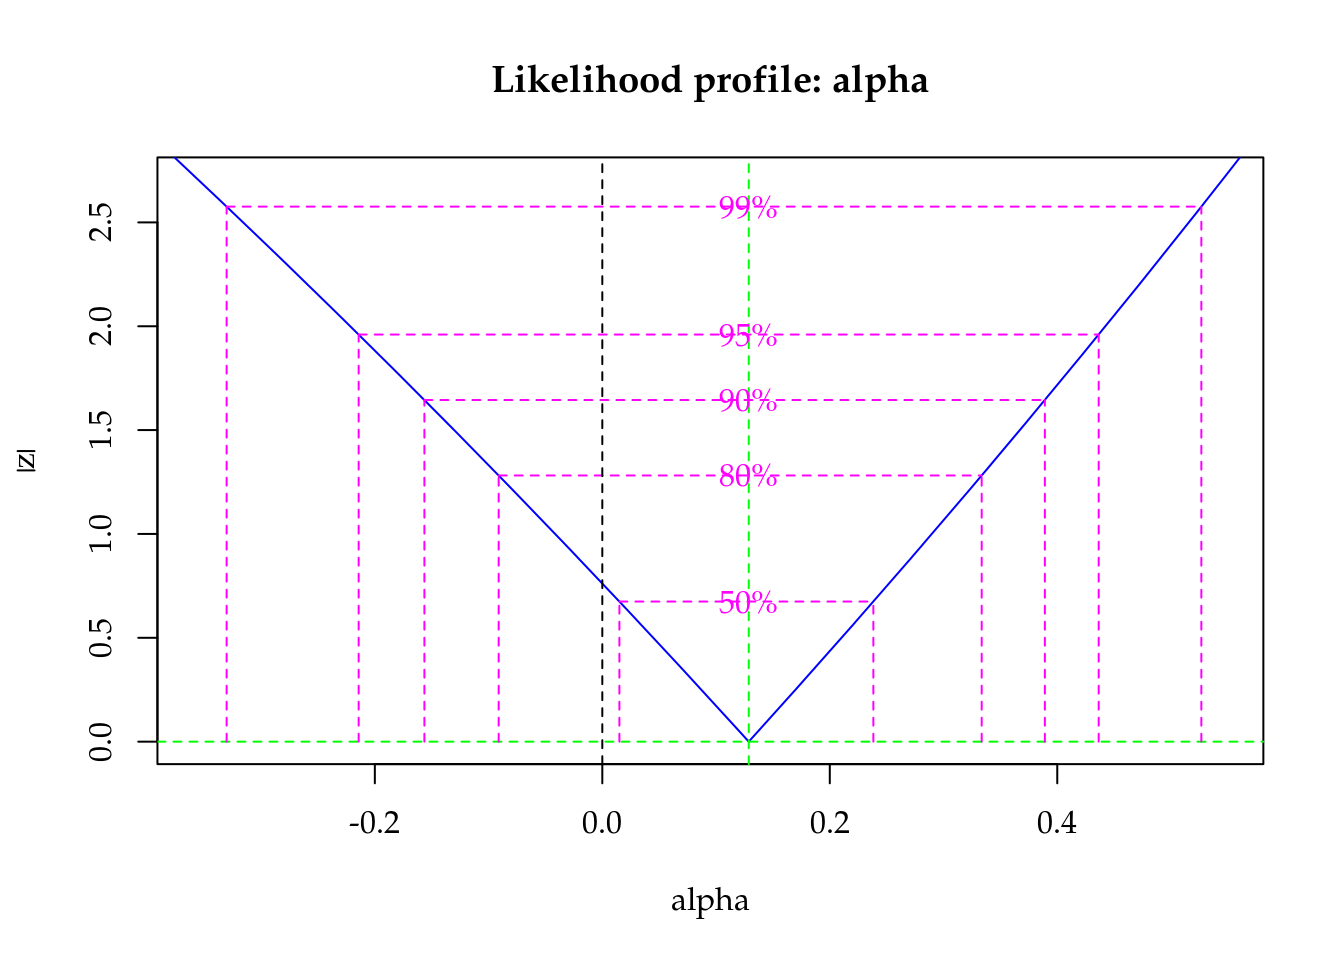
\includegraphics{rmcdbook_files/figure-latex/profile-alpha-pods-1} 

}

\caption{Profile log-likelihood for the Gamma-Count dispersion parameter. The confidence interval based on profile likelihood contains 0 inside as indicated by the solid vertical line.}\label{fig:profile-alpha-pods}
\end{figure}

The estimates and standard erros also were close on the (location)
regression parameters for all models. They differ only in the dispersion
parameter by construction.

\begin{Shaded}
\begin{Highlighting}[]
\NormalTok{c0 <-}\StringTok{ }\KeywordTok{summary}\NormalTok{(m0)$coefficients[, }\DecValTok{1}\NormalTok{:}\DecValTok{2}\NormalTok{]}
\NormalTok{c1 <-}\StringTok{ }\KeywordTok{summary}\NormalTok{(m1)@coef[, }\DecValTok{1}\NormalTok{:}\DecValTok{2}\NormalTok{]}
\NormalTok{c2 <-}\StringTok{ }\KeywordTok{rbind}\NormalTok{(}\KeywordTok{summary}\NormalTok{(m2)[[}\DecValTok{1}\NormalTok{]]$tau[, }\DecValTok{1}\NormalTok{:}\DecValTok{2}\NormalTok{],}
            \KeywordTok{summary}\NormalTok{(m2)[[}\DecValTok{1}\NormalTok{]]$Regression[, }\DecValTok{1}\NormalTok{:}\DecValTok{2}\NormalTok{])}
\end{Highlighting}
\end{Shaded}

\begin{Shaded}
\begin{Highlighting}[]
\CommentTok{# Parameter estimates according to each model.}
\NormalTok{c4 <-}\StringTok{ }\KeywordTok{cbind}\NormalTok{(}\StringTok{"P"} \NormalTok{=}\StringTok{ }\KeywordTok{rbind}\NormalTok{(}\OtherTok{NA}\NormalTok{, c0),}
            \StringTok{"GC"} \NormalTok{=}\StringTok{ }\NormalTok{c1,}
            \StringTok{"TW"} \NormalTok{=}\StringTok{ }\NormalTok{c2)}
\KeywordTok{colnames}\NormalTok{(c4) <-}\StringTok{ }\KeywordTok{substr}\NormalTok{(}\KeywordTok{colnames}\NormalTok{(c4), }\DecValTok{1}\NormalTok{, }\DecValTok{6}\NormalTok{)}
\KeywordTok{round}\NormalTok{(c4, }\DataTypeTok{digits =} \DecValTok{4}\NormalTok{)}
\end{Highlighting}
\end{Shaded}

\begin{verbatim}
##                P.Esti P.Std.  GC.Est GC.Std  TW.Est TW.Std
##                    NA     NA  0.1288 0.1655 -0.1088 0.1458
## (Intercept)    3.9537 0.0689  3.9549 0.0646  3.9537 0.0651
## blocII        -0.0293 0.0409 -0.0293 0.0383 -0.0293 0.0386
## blocIII       -0.0727 0.0414 -0.0726 0.0388 -0.0727 0.0390
## blocIV        -0.1254 0.0419 -0.1253 0.0393 -0.1254 0.0396
## blocV         -0.1079 0.0430 -0.1079 0.0403 -0.1079 0.0406
## umid50         0.1340 0.0877  0.1339 0.0822  0.1340 0.0827
## umid62,5       0.2166 0.0860  0.2163 0.0806  0.2166 0.0812
## K30            0.2743 0.0849  0.2740 0.0796  0.2743 0.0802
## K60            0.3080 0.0843  0.3076 0.0790  0.3080 0.0796
## K120           0.3288 0.0840  0.3285 0.0787  0.3288 0.0793
## K180           0.2554 0.0853  0.2551 0.0799  0.2554 0.0805
## umid50:K30     0.0632 0.1156  0.0632 0.1083  0.0632 0.1091
## umid62,5:K30  -0.1075 0.1154 -0.1073 0.1081 -0.1075 0.1089
## umid50:K60     0.1656 0.1137  0.1655 0.1066  0.1656 0.1073
## umid62,5:K60   0.1074 0.1122  0.1073 0.1052  0.1074 0.1059
## umid50:K120    0.1492 0.1134  0.1491 0.1063  0.1492 0.1070
## umid62,5:K120  0.1184 0.1140  0.1184 0.1069  0.1184 0.1077
## umid50:K180    0.3037 0.1136  0.3035 0.1065  0.3037 0.1072
## umid62,5:K180  0.1984 0.1126  0.1983 0.1055  0.1984 0.1063
\end{verbatim}

Until now, all models perform very close suggesting to keep the Poisson
by parsimony. But for testing purposes, Gamma-Count and Poisson-Tweedie
got a more significant p-value for the potassium amount \(\times\) soil
water content interaction. If a 5\% significance is adoted, models lead
to different practical conclusions.

\begin{Shaded}
\begin{Highlighting}[]
\CommentTok{# Analysis of deviance table.}
\KeywordTok{anova}\NormalTok{(m0, }\DataTypeTok{test =} \StringTok{"Chisq"}\NormalTok{)}
\end{Highlighting}
\end{Shaded}

\begin{verbatim}
## Analysis of Deviance Table
## 
## Model: poisson, link: log
## 
## Response: nvag
## 
## Terms added sequentially (first to last)
## 
## 
##        Df Deviance Resid. Df Resid. Dev Pr(>Chi)    
## NULL                      73        323             
## bloc    4     14.3        69        308   0.0064 ** 
## umid    2     92.9        67        215   <2e-16 ***
## K       4    136.1        63         79   <2e-16 ***
## umid:K  8     14.2        55         65   0.0779 .  
## ---
## Signif. codes:  0 '***' 0.001 '**' 0.01 '*' 0.05 '.' 0.1 ' ' 1
\end{verbatim}

\begin{Shaded}
\begin{Highlighting}[]
\CommentTok{# Wald test for interaction.}
\NormalTok{a <-}\StringTok{ }\KeywordTok{c}\NormalTok{(}\DecValTok{0}\NormalTok{, }\KeywordTok{attr}\NormalTok{(}\KeywordTok{model.matrix}\NormalTok{(m0), }\StringTok{"assign"}\NormalTok{))}
\NormalTok{ai <-}\StringTok{ }\NormalTok{a ==}\StringTok{ }\KeywordTok{max}\NormalTok{(a)}
\NormalTok{L <-}\StringTok{ }\KeywordTok{t}\NormalTok{(}\KeywordTok{replicate}\NormalTok{(}\KeywordTok{sum}\NormalTok{(ai), }\KeywordTok{rbind}\NormalTok{(}\KeywordTok{coef}\NormalTok{(m1) *}\StringTok{ }\DecValTok{0}\NormalTok{), }\DataTypeTok{simplify =} \StringTok{"matrix"}\NormalTok{))}
\NormalTok{L[, ai] <-}\StringTok{ }\KeywordTok{diag}\NormalTok{(}\KeywordTok{sum}\NormalTok{(ai))}
\KeywordTok{linearHypothesis}\NormalTok{(}\DataTypeTok{model =} \NormalTok{m0, }\CommentTok{# m0 is not being used here.}
                 \DataTypeTok{hypothesis.matrix =} \NormalTok{L,}
                 \DataTypeTok{vcov. =} \KeywordTok{vcov}\NormalTok{(m1),}
                 \DataTypeTok{coef. =} \KeywordTok{coef}\NormalTok{(m1))}
\end{Highlighting}
\end{Shaded}

\begin{verbatim}
## Linear hypothesis test
## 
## Hypothesis:
## umid50:K30 = 0
## umid62,5:K30 = 0
## umid50:K60 = 0
## umid62,5:K60 = 0
## umid50:K120 = 0
## umid62,5:K120 = 0
## umid50:K180 = 0
## umid62,5:K180 = 0
## 
## Model 1: restricted model
## Model 2: nvag ~ bloc + umid * K
## 
## Note: Coefficient covariance matrix supplied.
## 
##   Res.Df Df Chisq Pr(>Chisq)  
## 1     63                      
## 2     55  8    16      0.043 *
## ---
## Signif. codes:  0 '***' 0.001 '**' 0.01 '*' 0.05 '.' 0.1 ' ' 1
\end{verbatim}

\begin{Shaded}
\begin{Highlighting}[]
\CommentTok{# Wald test for fixed effects.}
\KeywordTok{anova}\NormalTok{(m2)}
\end{Highlighting}
\end{Shaded}

\begin{verbatim}
## Wald test for fixed effects
## Call: nvag ~ bloc + umid * K
## 
##    Covariate Chi.Square Df p.value
## 1     blocII      13.92  4  0.0076
## 2     umid50       7.15  2  0.0280
## 3        K30      20.93  4  0.0003
## 4 umid50:K30      15.76  8  0.0459
\end{verbatim}

Figure \ref{fig:segplot-pods} shows the estimated cells means with 95\%
confidence intervals. All estimated means are equals along models in
each cell. Gamma-count and Poisson-Tweedie have more shorter confidence
intervals than Poisson, because the extra flexibility enebled by fitting
a dispersion parameter.

\textbackslash{}begin\{figure\}{[}h{]}

\{\centering 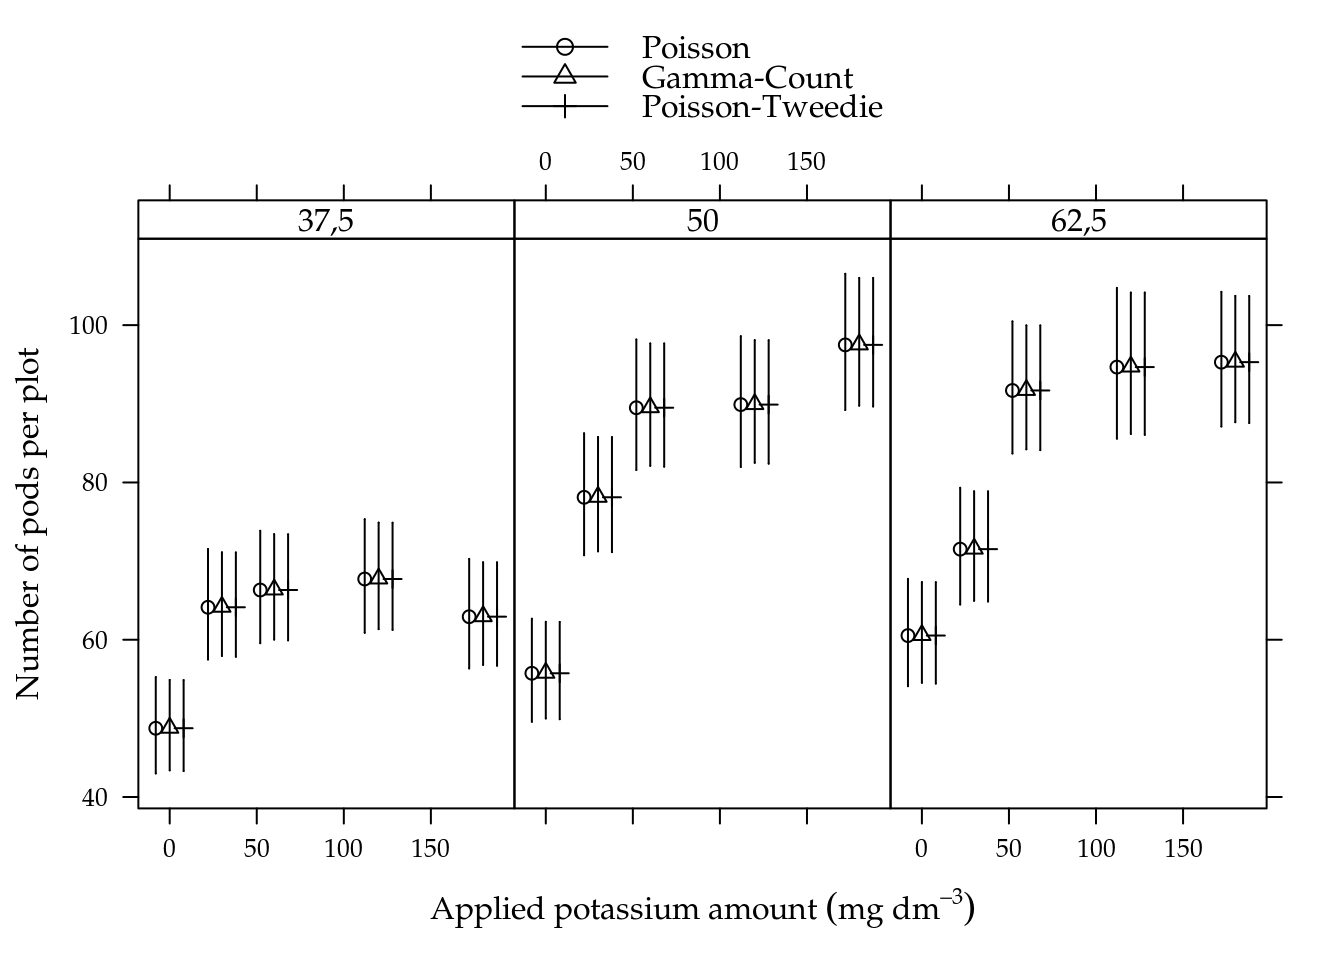
\includegraphics{rmcdbook_files/figure-latex/segplot-pods-1}

\}

\textbackslash{}caption\{Estimated cell means based on Poisson,
Gamma-Count and Poisson-Tweedie regression models. Segments are 95\%
individual coverage confidence intervals.\}\label{fig:segplot-pods}
\textbackslash{}end\{figure\}

We analysed the number of soybean pods. This variable showed
equidispersion than Gamma-Count and Poisson-Tweedie perform very close
to Poisson. For testing fixed effects, on the other hand, Poisson
weren't able to detect the interaction effect under a 5\% significance
level. This points out that more flexible models are powerful in
detecting effects.

\subsection{Number of grains}\label{number-of-grains}

For the analysis of number of beans, the same steps will be carried out,
just adaptating the code when needed. The first adaptation we need make
is to overcome a numerical problem in the Gamma-Count implementation.

The Gamma-Count mass function, and also the likelihood, computes the
difference of Gamma CDF. This difference can be numerically zero by lack
of precision and this leads to a -Inf in the log-likelihood. To overcame
this, we can use an artifitial offset that can prevent those zeros. The
code below shows the effect of offset on the probabilities.

\begin{Shaded}
\begin{Highlighting}[]
\NormalTok{dgcnt}
\end{Highlighting}
\end{Shaded}

\begin{verbatim}
## function (y, lambda, alpha) 
## {
##     p <- pgamma(q = 1, shape = y * alpha, rate = alpha * lambda) - 
##         pgamma(q = 1, shape = (y + 1) * alpha, rate = alpha * 
##             lambda)
##     return(p)
## }
## <environment: namespace:MRDCr>
\end{verbatim}

\begin{Shaded}
\begin{Highlighting}[]
\NormalTok{y <-}\StringTok{ }\DecValTok{0}\NormalTok{:}\DecValTok{30}
\NormalTok{lambda <-}\StringTok{ }\DecValTok{30}
\NormalTok{alpha <-}\StringTok{ }\DecValTok{5}
\NormalTok{off <-}\StringTok{ }\DecValTok{1}
\KeywordTok{pgamma}\NormalTok{(}\DataTypeTok{q =} \NormalTok{off,}
       \DataTypeTok{shape =} \NormalTok{y *}\StringTok{ }\NormalTok{alpha,}
       \DataTypeTok{rate =} \NormalTok{alpha *}\StringTok{ }\NormalTok{lambda) -}
\StringTok{    }\KeywordTok{pgamma}\NormalTok{(}\DataTypeTok{q =} \NormalTok{off,}
           \DataTypeTok{shape =} \NormalTok{(y +}\StringTok{ }\DecValTok{1}\NormalTok{) *}\StringTok{ }\NormalTok{alpha,}
           \DataTypeTok{rate =} \NormalTok{alpha *}\StringTok{ }\NormalTok{lambda)}
\end{Highlighting}
\end{Shaded}

\begin{verbatim}
##  [1] 0.00e+00 0.00e+00 0.00e+00 0.00e+00 0.00e+00 0.00e+00 0.00e+00
##  [8] 0.00e+00 0.00e+00 0.00e+00 0.00e+00 0.00e+00 1.78e-15 1.07e-13
## [15] 4.43e-12 1.32e-10 2.86e-09 4.62e-08 5.65e-07 5.31e-06 3.89e-05
## [22] 2.24e-04 1.03e-03 3.81e-03 1.14e-02 2.80e-02 5.67e-02 9.54e-02
## [29] 1.34e-01 1.59e-01 1.59e-01
\end{verbatim}

\begin{Shaded}
\begin{Highlighting}[]
\NormalTok{off <-}\StringTok{ }\NormalTok{off *}\StringTok{ }\FloatTok{0.5}
\KeywordTok{pgamma}\NormalTok{(}\DataTypeTok{q =} \NormalTok{off,}
       \DataTypeTok{shape =} \NormalTok{y *}\StringTok{ }\NormalTok{alpha,}
       \DataTypeTok{rate =} \NormalTok{alpha *}\StringTok{ }\NormalTok{lambda) -}
\StringTok{    }\KeywordTok{pgamma}\NormalTok{(}\DataTypeTok{q =} \NormalTok{off,}
           \DataTypeTok{shape =} \NormalTok{(y +}\StringTok{ }\DecValTok{1}\NormalTok{) *}\StringTok{ }\NormalTok{alpha,}
           \DataTypeTok{rate =} \NormalTok{alpha *}\StringTok{ }\NormalTok{lambda)}
\end{Highlighting}
\end{Shaded}

\begin{verbatim}
##  [1] 0.00e+00 0.00e+00 0.00e+00 1.24e-14 6.30e-12 1.15e-09 9.09e-08
##  [8] 3.48e-06 7.10e-05 8.29e-04 5.87e-03 2.63e-02 7.76e-02 1.56e-01
## [15] 2.18e-01 2.19e-01 1.60e-01 8.68e-02 3.56e-02 1.12e-02 2.74e-03
## [22] 5.25e-04 8.00e-05 9.77e-06 9.67e-07 7.80e-08 5.18e-09 2.85e-10
## [29] 1.31e-11 5.03e-13 1.64e-14
\end{verbatim}

The practical implication of an artificial offset is changing the size
of the unit were the counts were observed, so the estimates are
multiples of the those with offset 1. To be consistent, we will the same
artifitial offset, 10, in all models. This offset, artifitially, assumes
that the count were observed as a sum of 10 pots.

\begin{Shaded}
\begin{Highlighting}[]
\NormalTok{soja$off <-}\StringTok{ }\DecValTok{10}
\KeywordTok{fivenum}\NormalTok{(}\KeywordTok{with}\NormalTok{(soja, ngra/off))}
\end{Highlighting}
\end{Shaded}

\begin{verbatim}
## [1]  9.2 14.7 17.1 21.6 27.1
\end{verbatim}

\begin{Shaded}
\begin{Highlighting}[]
\CommentTok{#--------------------------------------------}
\CommentTok{# Poisson.}

\NormalTok{m0 <-}\StringTok{ }\KeywordTok{glm}\NormalTok{(ngra ~}\StringTok{ }\KeywordTok{offset}\NormalTok{(}\KeywordTok{log}\NormalTok{(off)) +}\StringTok{ }\NormalTok{bloc +}\StringTok{ }\NormalTok{umid *}\StringTok{ }\NormalTok{K,}
          \DataTypeTok{data =} \NormalTok{soja,}
          \DataTypeTok{family =} \NormalTok{poisson)}

\CommentTok{#--------------------------------------------}
\CommentTok{# Gamma-Count.}

\NormalTok{m1 <-}\StringTok{ }\KeywordTok{gcnt}\NormalTok{(}\KeywordTok{formula}\NormalTok{(m0), }\DataTypeTok{data =} \NormalTok{soja)}

\CommentTok{#--------------------------------------------}
\CommentTok{# Tweedie.}

\NormalTok{m2 <-}\StringTok{ }\KeywordTok{mcglm}\NormalTok{(}\DataTypeTok{linear_pred =} \KeywordTok{c}\NormalTok{(ngra ~}\StringTok{ }\NormalTok{bloc +}\StringTok{ }\NormalTok{umid *}\StringTok{ }\NormalTok{K),}
            \DataTypeTok{matrix_pred =} \KeywordTok{list}\NormalTok{(}\KeywordTok{mc_id}\NormalTok{(}\DataTypeTok{data =} \NormalTok{soja)),}
            \DataTypeTok{link =} \StringTok{"log"}\NormalTok{,}
            \DataTypeTok{offset =} \KeywordTok{list}\NormalTok{(}\KeywordTok{log}\NormalTok{(soja$off)),}
            \DataTypeTok{variance =} \StringTok{"poisson_tweedie"}\NormalTok{,}
            \DataTypeTok{power_fixed =} \OtherTok{FALSE}\NormalTok{,}
            \DataTypeTok{data =} \NormalTok{soja,}
            \DataTypeTok{control_algorithm =} \KeywordTok{list}\NormalTok{(}\DataTypeTok{verbose =} \OtherTok{FALSE}\NormalTok{,}
                                     \DataTypeTok{max_iter =} \DecValTok{100}\NormalTok{,}
                                     \DataTypeTok{tunning =} \FloatTok{0.2}\NormalTok{,}
                                     \DataTypeTok{correct =} \OtherTok{FALSE}\NormalTok{))}
\end{Highlighting}
\end{Shaded}

\begin{verbatim}
## Automatic initial values selected.
\end{verbatim}

To fit Poisson Tweedie for number of beans, we set
\texttt{power\_fixed\ =\ FALSE} option, because the number of beans if a
more dispersed variable than number of pods. We used 0.2 for tunning to
get convergence.

\begin{figure}[h]

{\centering 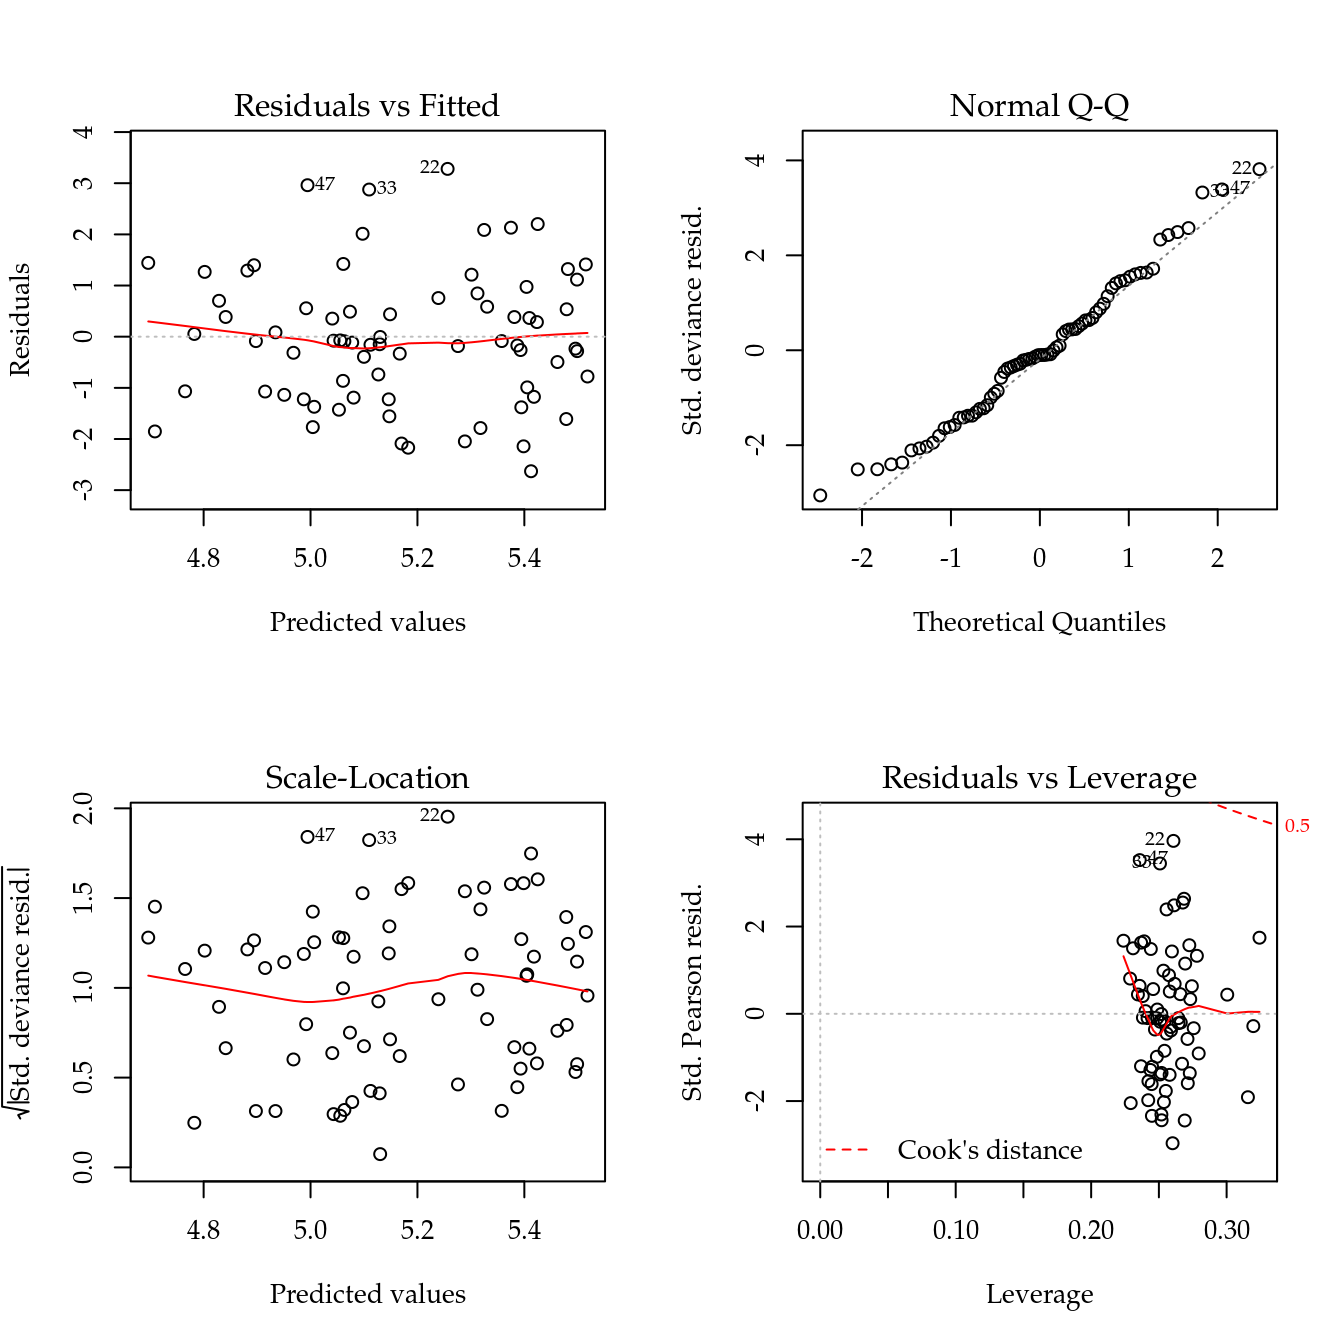
\includegraphics{rmcdbook_files/figure-latex/beans-plot-residuals-1} 

}

\caption{The 4 plots for checking departures of assumptions in the GLM-Poisson regression model for number of soybean pods.}\label{fig:beans-plot-residuals}
\end{figure}

Figure \ref{fig:beans-plot-residuals} shows the 4 plots based on
residuals. This residuals didn't show any departure pattern regarding
mispecification of the predictor (lack of fit, for example). The y axis
of the qq-norm plot has range on -3 to 4, indicating an overdispersed
count variable.

The maximised log-likelihood were different between Poisson and
Gamma-Count models. The profile log-likelihood for Gamma-Count
dispersion parameter does not contain 0 inside (Figure
\ref{fig:profile-alpha-beans}), so indicating a overdispersed case. The
profile show a simmetric shape with almost linear or ``V'' shape that
indicates a quadratic profile likelihood function.

\begin{Shaded}
\begin{Highlighting}[]
\CommentTok{#-----------------------------------------------------------------------}
\CommentTok{# Comparing models.}

\CommentTok{# Log-likelihood.}
\KeywordTok{c}\NormalTok{(}\DataTypeTok{P =} \KeywordTok{logLik}\NormalTok{(m0), }\DataTypeTok{GC =} \KeywordTok{logLik}\NormalTok{(m1), }\DataTypeTok{TW =} \OtherTok{NA}\NormalTok{)}
\end{Highlighting}
\end{Shaded}

\begin{verbatim}
##    P   GC   TW 
## -322 -316   NA
\end{verbatim}

\begin{Shaded}
\begin{Highlighting}[]
\NormalTok{cap <-}
\StringTok{    "Profile log-likelihood for the Gamma-Count dispersion parameter. The confidence interval based on profile likelihood contains 0 inside as indicated by the solid vertical line."}
\CommentTok{# Likelihhod profile for Gamma-Count dispersion parameter.}
\KeywordTok{plot}\NormalTok{(}\KeywordTok{profile}\NormalTok{(m1, }\DataTypeTok{which =} \StringTok{"alpha"}\NormalTok{))}
\end{Highlighting}
\end{Shaded}

\begin{figure}[h]

{\centering 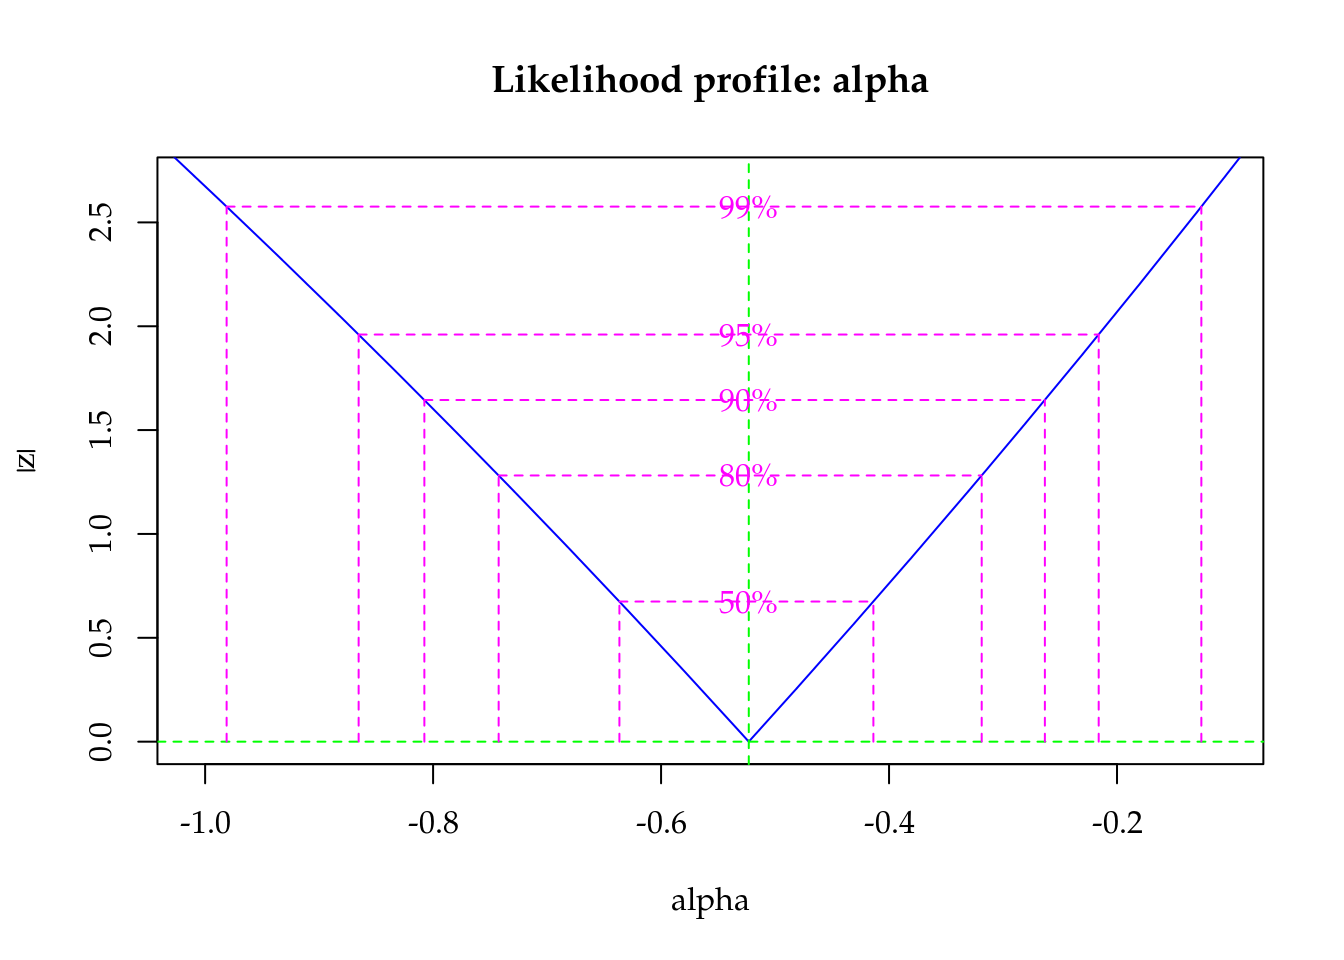
\includegraphics{rmcdbook_files/figure-latex/profile-alpha-beans-1} 

}

\caption{Profile log-likelihood for the Gamma-Count dispersion parameter. The confidence interval based on profile likelihood contains 0 inside as indicated by the solid vertical line.}\label{fig:profile-alpha-beans}
\end{figure}

The estimates for location parameters were the same for all three
models. The standard error for Poisson estimates were smaller than those
for Gamma-Count and Poisson-Tweedie. The ratio of standard errors
between Gamma-Count and Poisson were 1.3 (mean) and for Poisson-Tweedie
1.26 (mean).

\begin{Shaded}
\begin{Highlighting}[]
\NormalTok{c0 <-}\StringTok{ }\KeywordTok{summary}\NormalTok{(m0)$coefficients[, }\DecValTok{1}\NormalTok{:}\DecValTok{2}\NormalTok{]}
\NormalTok{c1 <-}\StringTok{ }\KeywordTok{summary}\NormalTok{(m1)@coef[, }\DecValTok{1}\NormalTok{:}\DecValTok{2}\NormalTok{]}
\NormalTok{c2 <-}\StringTok{ }\KeywordTok{rbind}\NormalTok{(}\KeywordTok{summary}\NormalTok{(m2)[[}\DecValTok{1}\NormalTok{]]$tau[, }\DecValTok{1}\NormalTok{:}\DecValTok{2}\NormalTok{],}
            \KeywordTok{summary}\NormalTok{(m2)[[}\DecValTok{1}\NormalTok{]]$Regression[, }\DecValTok{1}\NormalTok{:}\DecValTok{2}\NormalTok{])}
\end{Highlighting}
\end{Shaded}

\begin{Shaded}
\begin{Highlighting}[]
\CommentTok{# Parameter estimates according to each model.}
\NormalTok{c4 <-}\StringTok{ }\KeywordTok{cbind}\NormalTok{(}\StringTok{"P"} \NormalTok{=}\StringTok{ }\KeywordTok{rbind}\NormalTok{(}\OtherTok{NA}\NormalTok{, c0),}
            \StringTok{"GC"} \NormalTok{=}\StringTok{ }\NormalTok{c1,}
            \StringTok{"TW"} \NormalTok{=}\StringTok{ }\NormalTok{c2)}
\KeywordTok{colnames}\NormalTok{(c4) <-}\StringTok{ }\KeywordTok{substr}\NormalTok{(}\KeywordTok{colnames}\NormalTok{(c4), }\DecValTok{1}\NormalTok{, }\DecValTok{6}\NormalTok{)}
\KeywordTok{round}\NormalTok{(c4, }\DataTypeTok{digits =} \DecValTok{4}\NormalTok{)}
\end{Highlighting}
\end{Shaded}

\begin{verbatim}
##                P.Esti P.Std.  GC.Est GC.Std  TW.Est TW.Std
##                    NA     NA -0.5231 0.1651  0.0053 0.0314
## (Intercept)    2.4994 0.0448  2.4965 0.0582  2.4995 0.0549
## blocII        -0.0194 0.0266 -0.0194 0.0345 -0.0216 0.0352
## blocIII       -0.0366 0.0267 -0.0367 0.0347 -0.0376 0.0353
## blocIV        -0.1056 0.0272 -0.1058 0.0353 -0.1003 0.0356
## blocV         -0.0931 0.0279 -0.0933 0.0362 -0.0974 0.0365
## umid50         0.1325 0.0569  0.1328 0.0740  0.1333 0.0696
## umid62,5       0.1855 0.0562  0.1860 0.0731  0.1871 0.0690
## K30            0.2980 0.0549  0.2988 0.0713  0.2992 0.0678
## K60            0.3443 0.0543  0.3452 0.0706  0.3447 0.0674
## K120           0.3649 0.0541  0.3659 0.0703  0.3662 0.0672
## K180           0.2954 0.0549  0.2962 0.0714  0.2950 0.0679
## umid50:K30     0.0434 0.0748  0.0434 0.0973  0.0401 0.0936
## umid62,5:K30  -0.1367 0.0753 -0.1371 0.0979 -0.1392 0.0940
## umid50:K60     0.1156 0.0736  0.1157 0.0957  0.1146 0.0926
## umid62,5:K60   0.0917 0.0729  0.0917 0.0948  0.0896 0.0920
## umid50:K120    0.1186 0.0733  0.1187 0.0953  0.1184 0.0923
## umid62,5:K120  0.1627 0.0737  0.1628 0.0958  0.1591 0.0937
## umid50:K180    0.2883 0.0733  0.2887 0.0953  0.2884 0.0923
## umid62,5:K180  0.2157 0.0729  0.2159 0.0947  0.2142 0.0920
\end{verbatim}

\begin{Shaded}
\begin{Highlighting}[]
\CommentTok{# Ratios between stardard errors.}
\KeywordTok{cbind}\NormalTok{(}\DataTypeTok{GC =} \KeywordTok{summary}\NormalTok{(c4[-}\DecValTok{1}\NormalTok{, }\DecValTok{4}\NormalTok{]/c4[-}\DecValTok{1}\NormalTok{, }\DecValTok{2}\NormalTok{]),}
      \DataTypeTok{TW =} \KeywordTok{summary}\NormalTok{(c4[-}\DecValTok{1}\NormalTok{, }\DecValTok{6}\NormalTok{]/c4[-}\DecValTok{1}\NormalTok{, }\DecValTok{2}\NormalTok{]))}
\end{Highlighting}
\end{Shaded}

\begin{verbatim}
##          GC   TW
## Min.    1.3 1.22
## 1st Qu. 1.3 1.24
## Median  1.3 1.26
## Mean    1.3 1.26
## 3rd Qu. 1.3 1.27
## Max.    1.3 1.32
\end{verbatim}

The Poisson model gave the higher statistic to the rejection of the null
hypothesis than Gamma-Count and Poisson-Tweedie because it is assuming a
dispersion of 1 that is not the case. Gamma-Count and Poisson-Tweedie
perform very similar to test the interaction.

\begin{Shaded}
\begin{Highlighting}[]
\CommentTok{# Analysis of deviance table.}
\KeywordTok{anova}\NormalTok{(m0, }\DataTypeTok{test =} \StringTok{"Chisq"}\NormalTok{)}
\end{Highlighting}
\end{Shaded}

\begin{verbatim}
## Analysis of Deviance Table
## 
## Model: poisson, link: log
## 
## Response: ngra
## 
## Terms added sequentially (first to last)
## 
## 
##        Df Deviance Resid. Df Resid. Dev Pr(>Chi)    
## NULL                      73        761             
## bloc    4       28        69        733  1.1e-05 ***
## umid    2      185        67        548  < 2e-16 ***
## K       4      380        63        168  < 2e-16 ***
## umid:K  8       43        55        125  8.8e-07 ***
## ---
## Signif. codes:  0 '***' 0.001 '**' 0.01 '*' 0.05 '.' 0.1 ' ' 1
\end{verbatim}

\begin{Shaded}
\begin{Highlighting}[]
\CommentTok{# Wald test for interaction.}
\NormalTok{a <-}\StringTok{ }\KeywordTok{c}\NormalTok{(}\DecValTok{0}\NormalTok{, }\KeywordTok{attr}\NormalTok{(}\KeywordTok{model.matrix}\NormalTok{(m0), }\StringTok{"assign"}\NormalTok{))}
\NormalTok{ai <-}\StringTok{ }\NormalTok{a ==}\StringTok{ }\KeywordTok{max}\NormalTok{(a)}
\NormalTok{L <-}\StringTok{ }\KeywordTok{t}\NormalTok{(}\KeywordTok{replicate}\NormalTok{(}\KeywordTok{sum}\NormalTok{(ai), }\KeywordTok{rbind}\NormalTok{(}\KeywordTok{coef}\NormalTok{(m1) *}\StringTok{ }\DecValTok{0}\NormalTok{), }\DataTypeTok{simplify =} \StringTok{"matrix"}\NormalTok{))}
\NormalTok{L[, ai] <-}\StringTok{ }\KeywordTok{diag}\NormalTok{(}\KeywordTok{sum}\NormalTok{(ai))}
\KeywordTok{linearHypothesis}\NormalTok{(}\DataTypeTok{model =} \NormalTok{m0, }\CommentTok{# m0 is not being used here.}
                 \DataTypeTok{hypothesis.matrix =} \NormalTok{L,}
                 \DataTypeTok{vcov. =} \KeywordTok{vcov}\NormalTok{(m1),}
                 \DataTypeTok{coef. =} \KeywordTok{coef}\NormalTok{(m1))}
\end{Highlighting}
\end{Shaded}

\begin{verbatim}
## Linear hypothesis test
## 
## Hypothesis:
## umid50:K30 = 0
## umid62,5:K30 = 0
## umid50:K60 = 0
## umid62,5:K60 = 0
## umid50:K120 = 0
## umid62,5:K120 = 0
## umid50:K180 = 0
## umid62,5:K180 = 0
## 
## Model 1: restricted model
## Model 2: ngra ~ offset(log(off)) + bloc + umid * K
## 
## Note: Coefficient covariance matrix supplied.
## 
##   Res.Df Df Chisq Pr(>Chisq)   
## 1     63                       
## 2     55  8  25.3     0.0014 **
## ---
## Signif. codes:  0 '***' 0.001 '**' 0.01 '*' 0.05 '.' 0.1 ' ' 1
\end{verbatim}

\begin{Shaded}
\begin{Highlighting}[]
\CommentTok{# Wald test for fixed effects.}
\KeywordTok{anova}\NormalTok{(m2)}
\end{Highlighting}
\end{Shaded}

\begin{verbatim}
## Wald test for fixed effects
## Call: ngra ~ bloc + umid * K
## 
##    Covariate Chi.Square Df p.value
## 1     blocII      12.59  4  0.0134
## 2     umid50       7.68  2  0.0214
## 3        K30      36.96  4  0.0000
## 4 umid50:K30      25.56  8  0.0012
\end{verbatim}

Figure \ref{fig:segplot-beans} shows the estimated cells means with 95\%
confidence intervals. All estimated means are equals along models in
each cell. Gamma-count and Poisson-Tweedie have wider confidence
intervals than Poisson, because the extra variability where incorporated
on the model and have increased the estimates uncertainly.

\textbackslash{}begin\{figure\}{[}h{]}

\{\centering 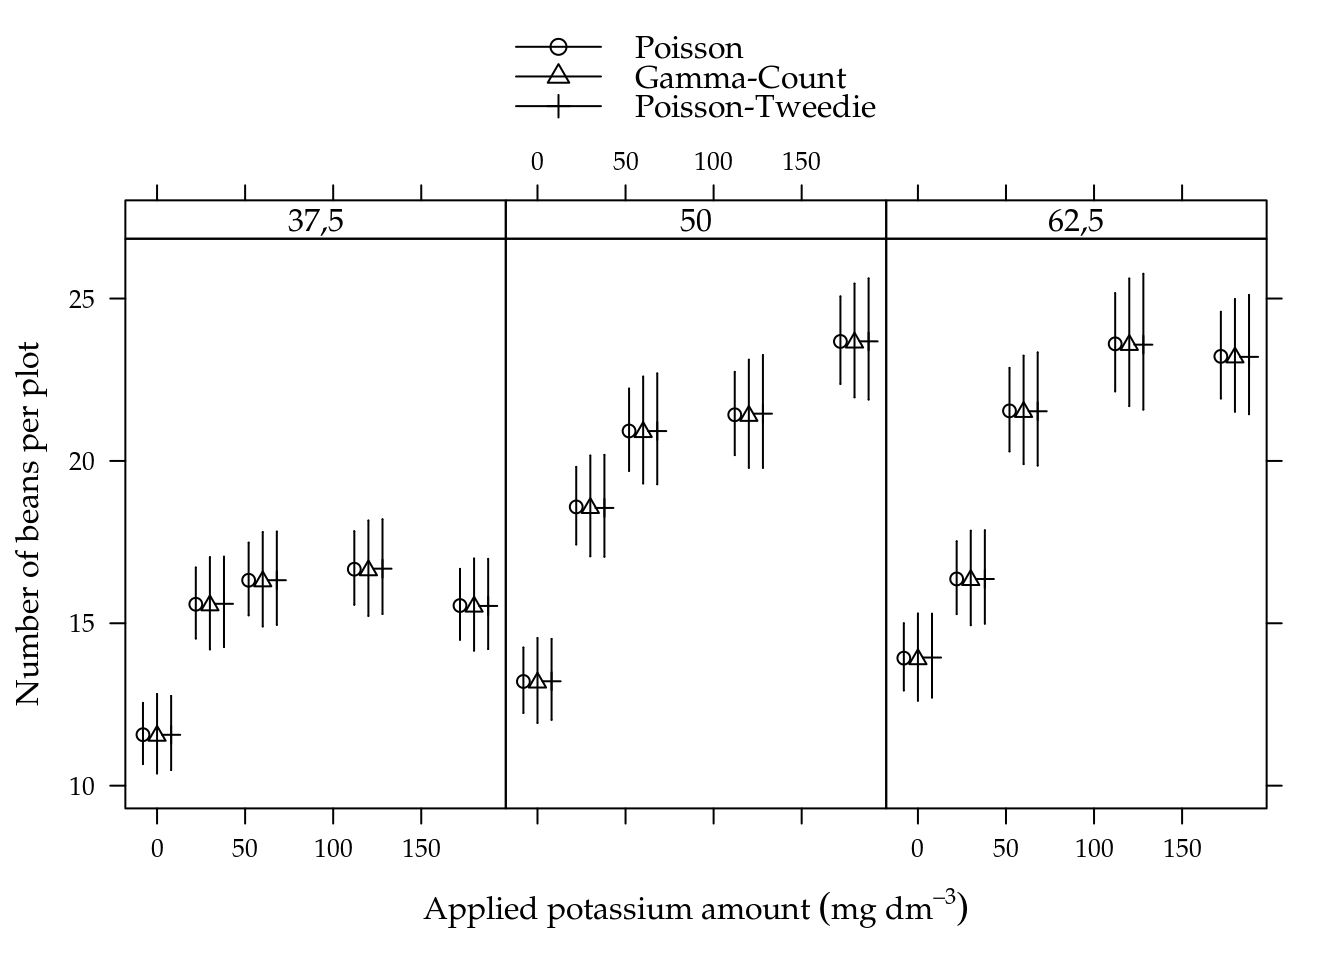
\includegraphics{rmcdbook_files/figure-latex/segplot-beans-1}

\}

\textbackslash{}caption\{Estimated cell means based on Poisson,
Gamma-Count and Poisson-Tweedie regression models. Segments are 95\%
individual coverage confidence intervals.\}\label{fig:segplot-beans}
\textbackslash{}end\{figure\}

We analysed the number of soybean beans. This variable showed slight
overdispersion. Gamma-count and Poisson-Tweedie performed very similiar.

\subsection{Number of grains per pod}\label{number-of-grains-per-pod}

Analyse the number of beans per plot is better than the total number of
beans, because the leter can be a side effect of the number of pods. We
will analyse the number of beans using the number of pods as an offset.

\begin{Shaded}
\begin{Highlighting}[]
\CommentTok{#--------------------------------------------}
\CommentTok{# Poisson.}

\NormalTok{m0 <-}\StringTok{ }\KeywordTok{glm}\NormalTok{(ngra ~}\StringTok{ }\KeywordTok{offset}\NormalTok{(}\KeywordTok{log}\NormalTok{(nvag)) +}\StringTok{ }\NormalTok{bloc +}\StringTok{ }\NormalTok{umid *}\StringTok{ }\NormalTok{K,}
          \DataTypeTok{data =} \NormalTok{soja,}
          \DataTypeTok{family =} \NormalTok{poisson)}

\CommentTok{#--------------------------------------------}
\CommentTok{# Gamma-Count.}

\NormalTok{m1 <-}\StringTok{ }\KeywordTok{gcnt}\NormalTok{(}\KeywordTok{formula}\NormalTok{(m0), }\DataTypeTok{data =} \NormalTok{soja)}

\CommentTok{#--------------------------------------------}
\CommentTok{# Tweedie.}

\NormalTok{m2 <-}\StringTok{ }\KeywordTok{mcglm}\NormalTok{(}\DataTypeTok{linear_pred =} \KeywordTok{c}\NormalTok{(ngra ~}\StringTok{ }\NormalTok{bloc +}\StringTok{ }\NormalTok{umid *}\StringTok{ }\NormalTok{K),}
            \DataTypeTok{matrix_pred =} \KeywordTok{list}\NormalTok{(}\KeywordTok{mc_id}\NormalTok{(}\DataTypeTok{data =} \NormalTok{soja)),}
            \DataTypeTok{link =} \StringTok{"log"}\NormalTok{,}
            \DataTypeTok{offset =} \KeywordTok{list}\NormalTok{(}\KeywordTok{log}\NormalTok{(soja$nvag)),}
            \DataTypeTok{variance =} \StringTok{"poisson_tweedie"}\NormalTok{,}
            \DataTypeTok{power_fixed =} \OtherTok{TRUE}\NormalTok{,}
            \DataTypeTok{data =} \NormalTok{soja,}
            \DataTypeTok{control_algorithm =} \KeywordTok{list}\NormalTok{(}\DataTypeTok{verbose =} \OtherTok{FALSE}\NormalTok{,}
                                     \DataTypeTok{max_iter =} \DecValTok{100}\NormalTok{,}
                                     \DataTypeTok{tunning =} \FloatTok{0.5}\NormalTok{,}
                                     \DataTypeTok{correct =} \OtherTok{FALSE}\NormalTok{))}
\end{Highlighting}
\end{Shaded}

\begin{verbatim}
## Automatic initial values selected.
\end{verbatim}

To accomplish the fitting, we set \texttt{power\_fixed\ =\ TRUE}
otherwise convergence wasn't met.

\begin{figure}[h]

{\centering 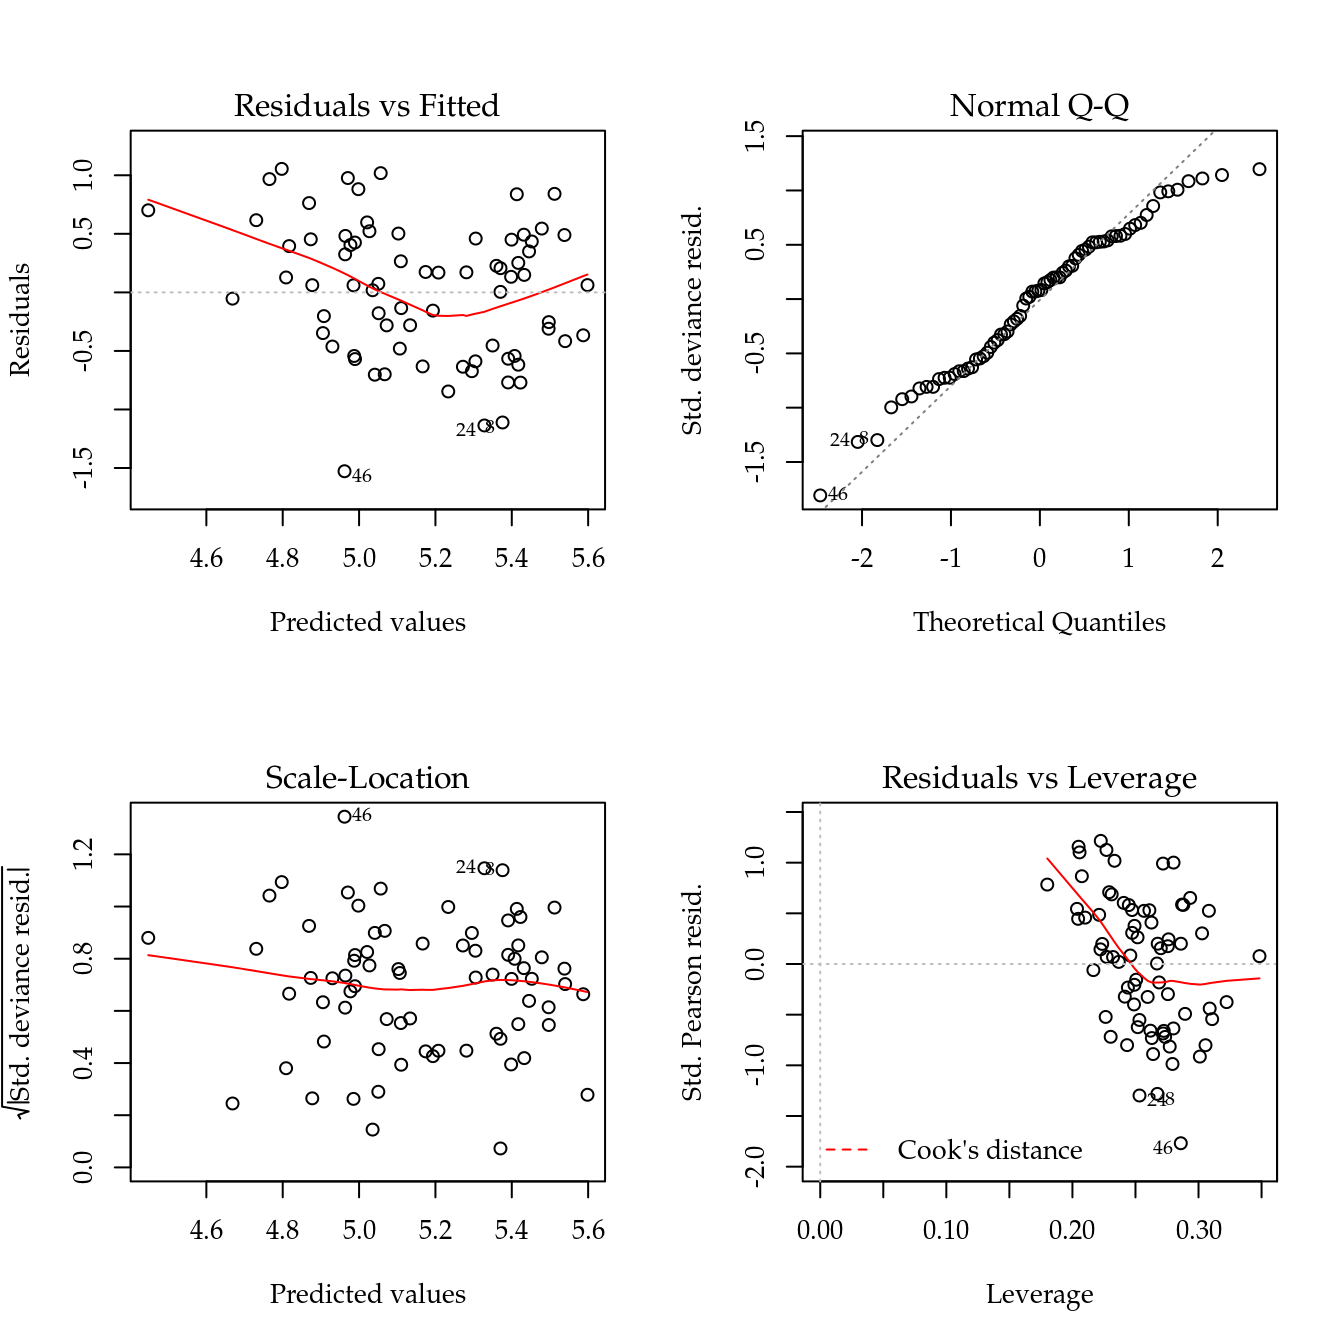
\includegraphics{rmcdbook_files/figure-latex/bp-plot-residuals-1} 

}

\caption{The 4 plots for checking departures of assumptions in the GLM-Poisson regression model for number of soybean pods.}\label{fig:bp-plot-residuals}
\end{figure}

Figure \ref{fig:bp-plot-residuals} shows the 4 plots based on residuals.
The y axis of the qq-norm plot has range on -1.5 to 1.5, indicating an
underdispersed count variable.

The maximised log-likelihood were different between Poisson and
Gamma-Count models. The profile log-likelihood for Gamma-Count
dispersion parameter does not contain 0 inside (Figure
\ref{fig:profile-alpha-bp}), so indicating an underdispersed count. The
profile likelihood is ``V'' shape that represents a quadratic profile
log-likelihood function.

\begin{Shaded}
\begin{Highlighting}[]
\CommentTok{#-----------------------------------------------------------------------}
\CommentTok{# Comparing models.}

\CommentTok{# Log-likelihood.}
\KeywordTok{c}\NormalTok{(}\DataTypeTok{P =} \KeywordTok{logLik}\NormalTok{(m0), }\DataTypeTok{GC =} \KeywordTok{logLik}\NormalTok{(m1), }\DataTypeTok{TW =} \OtherTok{NA}\NormalTok{)}
\end{Highlighting}
\end{Shaded}

\begin{verbatim}
##    P   GC   TW 
## -271 -255   NA
\end{verbatim}

\begin{Shaded}
\begin{Highlighting}[]
\NormalTok{cap <-}
\StringTok{    "Profile log-likelihood for the Gamma-Count dispersion parameter. The confidence interval based on profile likelihood contains 0 inside as indicated by the solid vertical line."}
\CommentTok{# Likelihhod profile for Gamma-Count dispersion parameter.}
\KeywordTok{plot}\NormalTok{(}\KeywordTok{profile}\NormalTok{(m1, }\DataTypeTok{which =} \StringTok{"alpha"}\NormalTok{))}
\end{Highlighting}
\end{Shaded}

\begin{figure}[h]

{\centering 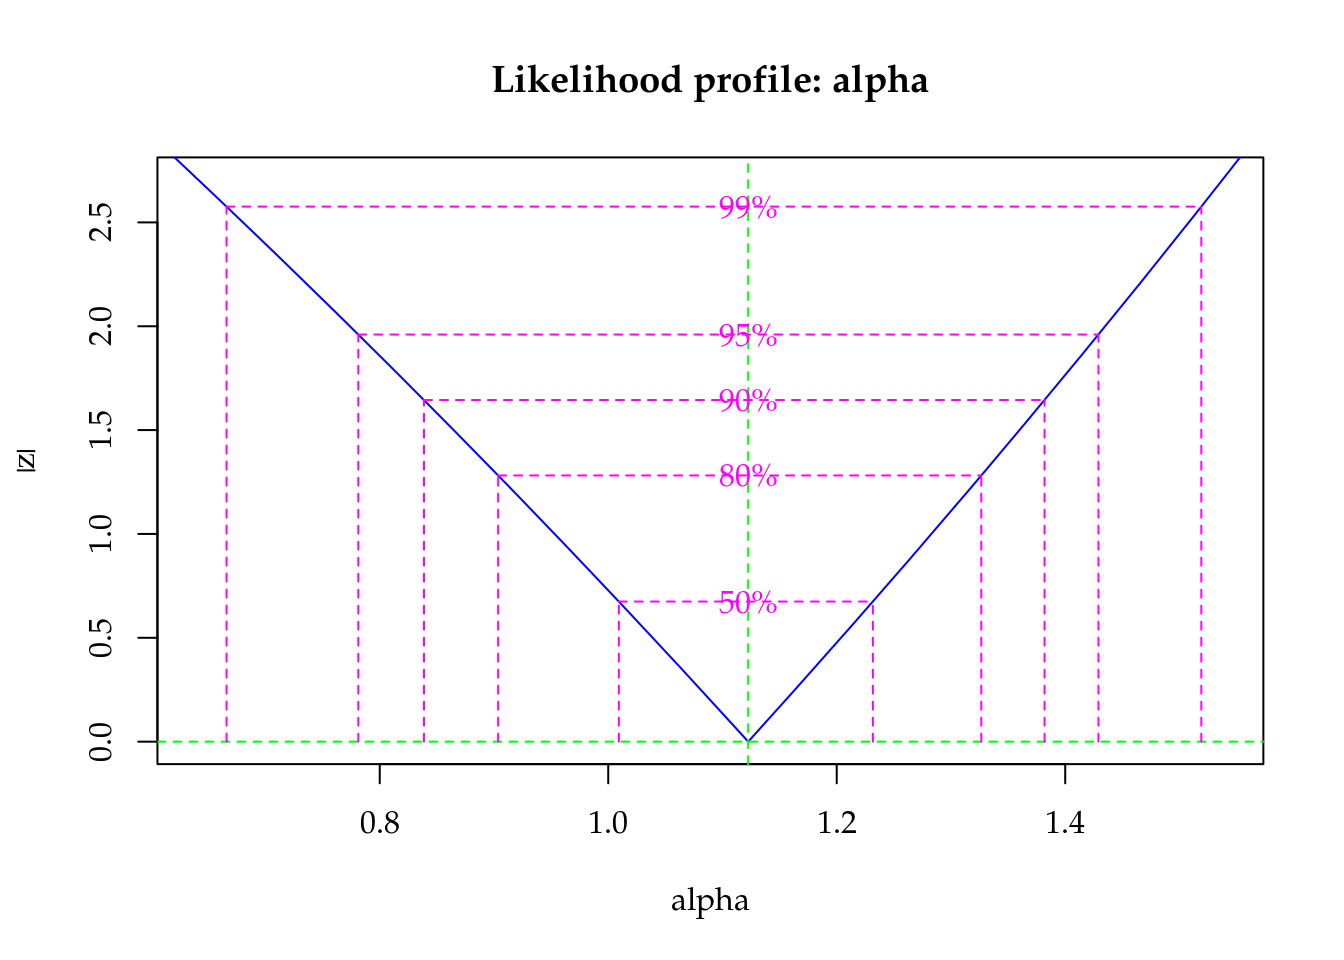
\includegraphics{rmcdbook_files/figure-latex/profile-alpha-bp-1} 

}

\caption{Profile log-likelihood for the Gamma-Count dispersion parameter. The confidence interval based on profile likelihood contains 0 inside as indicated by the solid vertical line.}\label{fig:profile-alpha-bp}
\end{figure}

The point estimates for location parameters were, once more, the same
for all three models. The standard error for Poisson estimates were
greater than those for Gamma-Count and Poisson-Tweedie.

\begin{Shaded}
\begin{Highlighting}[]
\NormalTok{c0 <-}\StringTok{ }\KeywordTok{summary}\NormalTok{(m0)$coefficients[, }\DecValTok{1}\NormalTok{:}\DecValTok{2}\NormalTok{]}
\NormalTok{c1 <-}\StringTok{ }\KeywordTok{summary}\NormalTok{(m1)@coef[, }\DecValTok{1}\NormalTok{:}\DecValTok{2}\NormalTok{]}
\NormalTok{c2 <-}\StringTok{ }\KeywordTok{rbind}\NormalTok{(}\KeywordTok{summary}\NormalTok{(m2)[[}\DecValTok{1}\NormalTok{]]$tau[, }\DecValTok{1}\NormalTok{:}\DecValTok{2}\NormalTok{],}
            \KeywordTok{summary}\NormalTok{(m2)[[}\DecValTok{1}\NormalTok{]]$Regression[, }\DecValTok{1}\NormalTok{:}\DecValTok{2}\NormalTok{])}
\end{Highlighting}
\end{Shaded}

\begin{Shaded}
\begin{Highlighting}[]
\CommentTok{# Parameter estimates according to each model.}
\NormalTok{c4 <-}\StringTok{ }\KeywordTok{cbind}\NormalTok{(}\StringTok{"P"} \NormalTok{=}\StringTok{ }\KeywordTok{rbind}\NormalTok{(}\OtherTok{NA}\NormalTok{, c0),}
            \StringTok{"GC"} \NormalTok{=}\StringTok{ }\NormalTok{c1,}
            \StringTok{"TW"} \NormalTok{=}\StringTok{ }\NormalTok{c2)}
\KeywordTok{colnames}\NormalTok{(c4) <-}\StringTok{ }\KeywordTok{substr}\NormalTok{(}\KeywordTok{colnames}\NormalTok{(c4), }\DecValTok{1}\NormalTok{, }\DecValTok{6}\NormalTok{)}
\KeywordTok{round}\NormalTok{(c4, }\DataTypeTok{digits =} \DecValTok{4}\NormalTok{)}
\end{Highlighting}
\end{Shaded}

\begin{verbatim}
##                P.Esti P.Std.  GC.Est GC.Std  TW.Est TW.Std
##                    NA     NA  1.1225 0.1648 -0.6764 0.0446
## (Intercept)    0.8482 0.0447  0.8510 0.0255  0.8482 0.0254
## blocII         0.0113 0.0266  0.0114 0.0152  0.0113 0.0151
## blocIII        0.0363 0.0267  0.0363 0.0152  0.0363 0.0152
## blocIV         0.0194 0.0272  0.0195 0.0155  0.0194 0.0155
## blocV          0.0161 0.0280  0.0163 0.0159  0.0161 0.0159
## umid50        -0.0019 0.0569 -0.0023 0.0325 -0.0019 0.0324
## umid62,5      -0.0312 0.0563 -0.0317 0.0321 -0.0312 0.0320
## K30            0.0229 0.0549  0.0221 0.0313  0.0229 0.0312
## K60            0.0345 0.0544  0.0337 0.0310  0.0345 0.0309
## K120           0.0353 0.0541  0.0344 0.0309  0.0353 0.0308
## K180           0.0406 0.0549  0.0399 0.0313  0.0406 0.0312
## umid50:K30    -0.0187 0.0748 -0.0187 0.0427 -0.0187 0.0426
## umid62,5:K30  -0.0285 0.0753 -0.0281 0.0429 -0.0285 0.0428
## umid50:K60    -0.0482 0.0736 -0.0483 0.0420 -0.0482 0.0419
## umid62,5:K60  -0.0140 0.0729 -0.0140 0.0416 -0.0140 0.0415
## umid50:K120   -0.0304 0.0733 -0.0305 0.0418 -0.0304 0.0417
## umid62,5:K120  0.0455 0.0738  0.0454 0.0421  0.0455 0.0420
## umid50:K180   -0.0163 0.0733 -0.0167 0.0418 -0.0163 0.0417
## umid62,5:K180  0.0169 0.0729  0.0167 0.0416  0.0169 0.0415
\end{verbatim}

\begin{Shaded}
\begin{Highlighting}[]
\CommentTok{# Ratios between stardard errors.}
\KeywordTok{cbind}\NormalTok{(}\DataTypeTok{GC =} \KeywordTok{summary}\NormalTok{(c4[-}\DecValTok{1}\NormalTok{, }\DecValTok{4}\NormalTok{]/c4[-}\DecValTok{1}\NormalTok{, }\DecValTok{2}\NormalTok{]),}
      \DataTypeTok{TW =} \KeywordTok{summary}\NormalTok{(c4[-}\DecValTok{1}\NormalTok{, }\DecValTok{6}\NormalTok{]/c4[-}\DecValTok{1}\NormalTok{, }\DecValTok{2}\NormalTok{]))}
\end{Highlighting}
\end{Shaded}

\begin{verbatim}
##           GC    TW
## Min.    0.57 0.569
## 1st Qu. 0.57 0.569
## Median  0.57 0.569
## Mean    0.57 0.569
## 3rd Qu. 0.57 0.569
## Max.    0.57 0.569
\end{verbatim}

None of the experimental factors had effect on the number of beans per
pod. Althought, Gamma-Count and Poisson-Tweedie showed more favorable
statistics to the rejection of the null hypothesis than Poisson.

\begin{Shaded}
\begin{Highlighting}[]
\CommentTok{# Analysis of deviance table.}
\KeywordTok{anova}\NormalTok{(m0, }\DataTypeTok{test =} \StringTok{"Chisq"}\NormalTok{)}
\end{Highlighting}
\end{Shaded}

\begin{verbatim}
## Analysis of Deviance Table
## 
## Model: poisson, link: log
## 
## Response: ngra
## 
## Terms added sequentially (first to last)
## 
## 
##        Df Deviance Resid. Df Resid. Dev Pr(>Chi)
## NULL                      73       34.2         
## bloc    4     2.03        69       32.2     0.73
## umid    2     1.75        67       30.5     0.42
## K       4     3.83        63       26.6     0.43
## umid:K  8     2.65        55       24.0     0.95
\end{verbatim}

\begin{Shaded}
\begin{Highlighting}[]
\CommentTok{# Wald test for interaction.}
\NormalTok{a <-}\StringTok{ }\KeywordTok{c}\NormalTok{(}\DecValTok{0}\NormalTok{, }\KeywordTok{attr}\NormalTok{(}\KeywordTok{model.matrix}\NormalTok{(m0), }\StringTok{"assign"}\NormalTok{))}
\NormalTok{ai <-}\StringTok{ }\NormalTok{a ==}\StringTok{ }\KeywordTok{max}\NormalTok{(a)}
\NormalTok{L <-}\StringTok{ }\KeywordTok{t}\NormalTok{(}\KeywordTok{replicate}\NormalTok{(}\KeywordTok{sum}\NormalTok{(ai), }\KeywordTok{rbind}\NormalTok{(}\KeywordTok{coef}\NormalTok{(m1) *}\StringTok{ }\DecValTok{0}\NormalTok{), }\DataTypeTok{simplify =} \StringTok{"matrix"}\NormalTok{))}
\NormalTok{L[, ai] <-}\StringTok{ }\KeywordTok{diag}\NormalTok{(}\KeywordTok{sum}\NormalTok{(ai))}
\KeywordTok{linearHypothesis}\NormalTok{(}\DataTypeTok{model =} \NormalTok{m0, }\CommentTok{# m0 is not being used here.}
                 \DataTypeTok{hypothesis.matrix =} \NormalTok{L,}
                 \DataTypeTok{vcov. =} \KeywordTok{vcov}\NormalTok{(m1),}
                 \DataTypeTok{coef. =} \KeywordTok{coef}\NormalTok{(m1))}
\end{Highlighting}
\end{Shaded}

\begin{verbatim}
## Linear hypothesis test
## 
## Hypothesis:
## umid50:K30 = 0
## umid62,5:K30 = 0
## umid50:K60 = 0
## umid62,5:K60 = 0
## umid50:K120 = 0
## umid62,5:K120 = 0
## umid50:K180 = 0
## umid62,5:K180 = 0
## 
## Model 1: restricted model
## Model 2: ngra ~ offset(log(nvag)) + bloc + umid * K
## 
## Note: Coefficient covariance matrix supplied.
## 
##   Res.Df Df Chisq Pr(>Chisq)
## 1     63                    
## 2     55  8   8.1       0.42
\end{verbatim}

\begin{Shaded}
\begin{Highlighting}[]
\CommentTok{# Wald test for fixed effects.}
\KeywordTok{anova}\NormalTok{(m2)}
\end{Highlighting}
\end{Shaded}

\begin{verbatim}
## Wald test for fixed effects
## Call: ngra ~ bloc + umid * K
## 
##    Covariate Chi.Square Df p.value
## 1     blocII       6.03  4   0.197
## 2     umid50       1.26  2   0.534
## 3        K30       2.09  4   0.719
## 4 umid50:K30       8.20  8   0.414
\end{verbatim}

Figure \ref{fig:segplot-bp} shows the estimated cells means with 95\%
confidence intervals. All estimated means are equals along models in
each cell. Gamma-count and Poisson-Tweedie have more shorter confidence
intervals than Poisson.

\textbackslash{}begin\{figure\}{[}h{]}

\{\centering 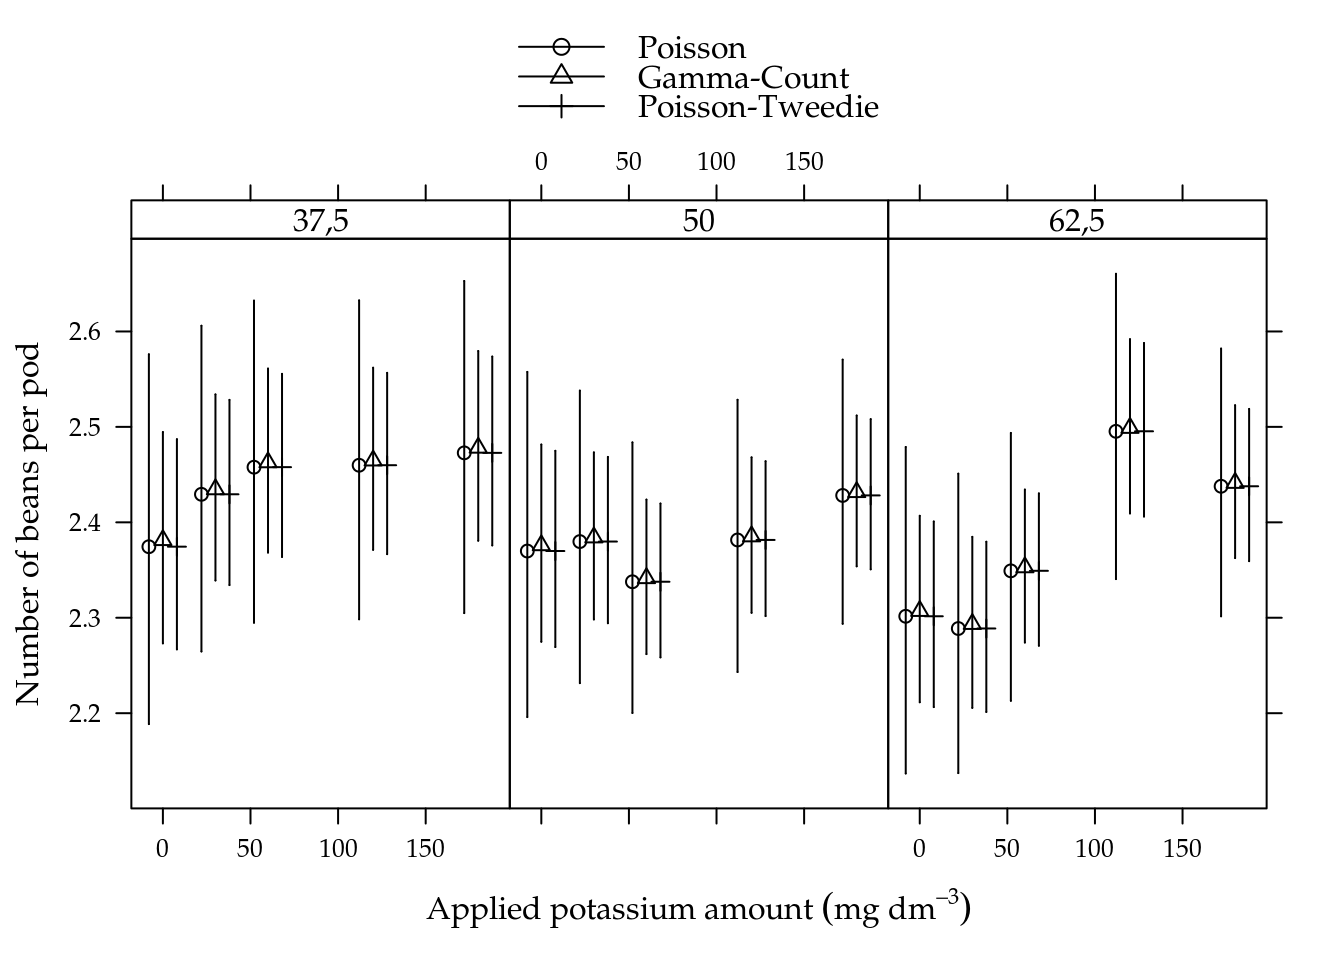
\includegraphics{rmcdbook_files/figure-latex/segplot-bp-1}

\}

\textbackslash{}caption\{Estimated cell means based on Poisson,
Gamma-Count and Poisson-Tweedie regression models. Segments are 95\%
individual coverage confidence intervals.\}\label{fig:segplot-bp}
\textbackslash{}end\{figure\}

We analysed the number of beans por pod in a experiment with soybeans.
This variable showed underdispersion so Gamma-Count and Poisson-Tweedie
perform better than Poisson.

\section{Number of vehicle claims}\label{number-of-vehicle-claims}

Em companhias de seguros é de fundamental importância especificar um
preço adequado correspondente a um segurado, a fim de cobrir o risco
assumido. Tal tarefa geralmente envolve a avaliação de características
do plano de seguro que influenciam na taxa de sinistros observada.

Nesta seção nós apresentamos a análise de um conjunto do dados
referentes ao acompanhamento de 16483 clientes de uma seguradora de
veículos ao longo de um ano. Os dados estão disponíveis no pacote
\texttt{MRDCr} (com documentação em português) e podem ser carregados
com

\begin{Shaded}
\begin{Highlighting}[]
\NormalTok{##----------------------------------------------------------------------}
\NormalTok{## Load and organize data}
\KeywordTok{data}\NormalTok{(}\DataTypeTok{package =} \StringTok{"MRDCr"}\NormalTok{)}
\KeywordTok{help}\NormalTok{(seguros, }\DataTypeTok{h =} \StringTok{"html"}\NormalTok{)}
\end{Highlighting}
\end{Shaded}

Após a tradução dos níveis das variáveis categóricas a estrutura dos
dados fica

\begin{Shaded}
\begin{Highlighting}[]
\NormalTok{## Translate levels of categorical variables and colnames}
\KeywordTok{colnames}\NormalTok{(seguros) <-}\StringTok{ }\KeywordTok{c}\NormalTok{(}\StringTok{"age"}\NormalTok{, }\StringTok{"sex"}\NormalTok{, }\StringTok{"price"}\NormalTok{, }\StringTok{"expo"}\NormalTok{, }\StringTok{"nclaims"}\NormalTok{)}
\KeywordTok{levels}\NormalTok{(seguros$sex) <-}\StringTok{ }\KeywordTok{c}\NormalTok{(}\StringTok{"Female"}\NormalTok{, }\StringTok{"Male"}\NormalTok{)}
\KeywordTok{str}\NormalTok{(seguros)}
\end{Highlighting}
\end{Shaded}

\begin{verbatim}
## 'data.frame':    16483 obs. of  5 variables:
##  $ age    : int  59 45 42 63 36 33 35 63 54 32 ...
##  $ sex    : Factor w/ 2 levels "Female","Male": 1 2 2 1 1 2 2 2 2 2 ...
##  $ price  : num  24.6 23.4 86.6 77.5 25.9 ...
##  $ expo   : num  0.5 0.7 0.79 0.01 0.51 0.79 0.81 0.01 0.76 0.79 ...
##  $ nclaims: int  1 0 0 0 0 0 0 0 0 0 ...
\end{verbatim}

In this dataset a variável \texttt{age} é mensurada em anos, e
\texttt{price} em 1000 reais. A variável \texttt{expo} representa o
período de cobertura do cliente, durante o ano sob análise, um valor de
0.5 significa que o cliente esteve exposto ao sinistro durante metade do
ano.

A Figura \ref{fig:desc-claim} mostra a descrição das variáveis a serem
utilizadas na análise. Embora esses gráficos não considerem todas as
variáveis conjuntamente, o gráfico à esquerda sugere que há um excesso
de contagens nulas, no geral 95.183\% das contagens são 0.

\begin{figure}[h]

{\centering 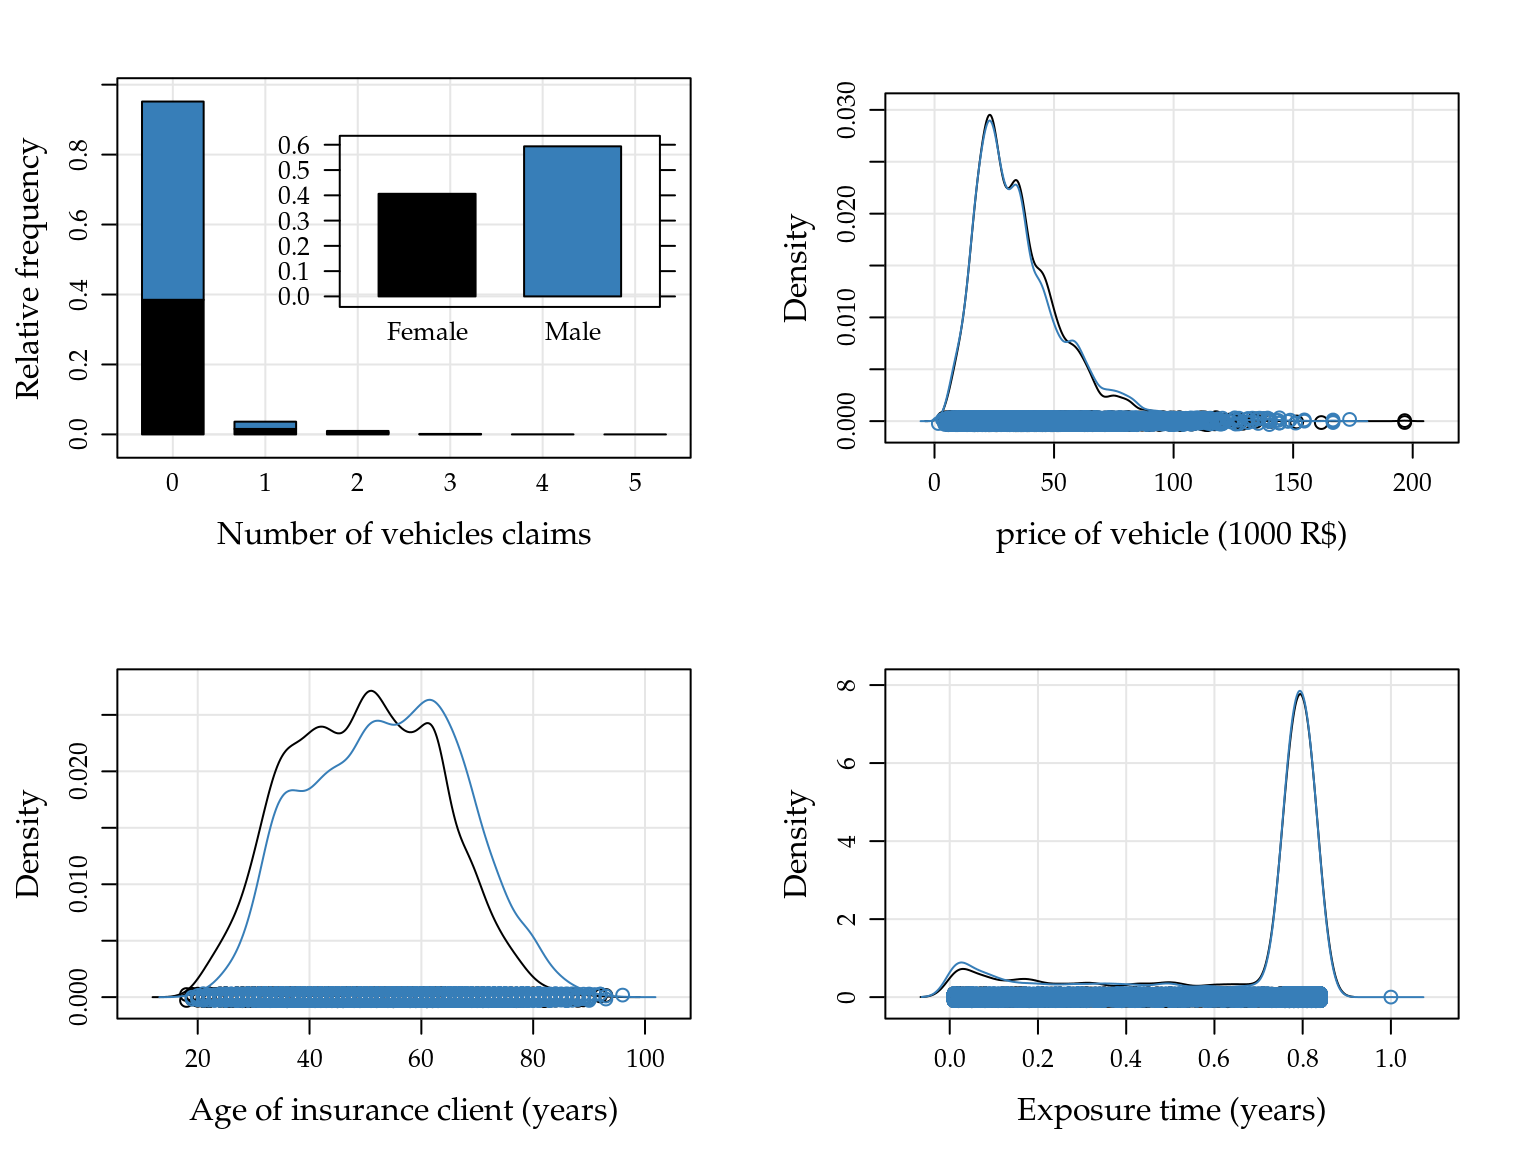
\includegraphics{rmcdbook_files/figure-latex/desc-claim-1} 

}

\caption{Relative frequencies for number of vehicle claims, and empirical densities to price of vehicle, age of clients and exposure time by sex of insurance clients.}\label{fig:desc-claim}
\end{figure}

Para análise desses dados consideramos efeitos quadráticos para
variáveis contínuas e intercepto variando conforme sexo do cliente.
\texttt{price} foi tomada como preditor pode ser escrito como

\begin{equation*}
  \begin{split}
  \log\left ( \frac{\mu_i}{\texttt{expo}_i} \right ) = &
  \beta_0 + \beta_1 \mathbb{1}(\texttt{sex}_i) +
  \beta_2 \texttt{price}_i + \\
  & + \beta_3 \texttt{price}_i^2 +
  \beta_4 \texttt{age}_i +
  \beta_5 \texttt{age}_i^2
  \end{split}
\end{equation*}

em R definimos o preditor conforme sintaxe para objetos da classe
\texttt{formula}. Note que a variável \texttt{expo} é envolta na função
\texttt{offset} e sendo assim é considerado apenas como denominador das
contagens.

\begin{Shaded}
\begin{Highlighting}[]
\NormalTok{## Define preditor}
\NormalTok{form0 <-}\StringTok{ }\NormalTok{nclaims ~}\StringTok{ }\KeywordTok{offset}\NormalTok{(}\KeywordTok{log}\NormalTok{(expo)) +}\StringTok{ }\NormalTok{sex +}
\StringTok{    }\NormalTok{price +}\StringTok{ }\KeywordTok{I}\NormalTok{(price^}\DecValTok{2}\NormalTok{) +}\StringTok{ }\NormalTok{age +}\StringTok{ }\KeywordTok{I}\NormalTok{(age^}\DecValTok{2}\NormalTok{)}
\end{Highlighting}
\end{Shaded}

Nós ajustamos os modelos de regressão Poisson e Poisson-Tweedie usando
os frameworks \texttt{stats::glm} e \texttt{mcglm::mcglm}, que se baseam
em máxima verossimilhança e especificação por momentos respectivamente.

\begin{Shaded}
\begin{Highlighting}[]
\NormalTok{## Fit Poisson}
\NormalTok{m0PO <-}\StringTok{ }\KeywordTok{glm}\NormalTok{(form0, }\DataTypeTok{data =} \NormalTok{seguros, }\DataTypeTok{family =} \NormalTok{poisson)}

\NormalTok{## Fit Poisson-Tweedie}
\NormalTok{m0PT <-}\StringTok{ }\KeywordTok{mcglm}\NormalTok{(}
    \DataTypeTok{linear_pred =} \KeywordTok{c}\NormalTok{(form0),}
    \DataTypeTok{matrix_pred =} \KeywordTok{list}\NormalTok{(}\KeywordTok{mc_id}\NormalTok{(seguros)),}
    \DataTypeTok{link =} \StringTok{"log"}\NormalTok{,}
    \DataTypeTok{variance =} \StringTok{"poisson_tweedie"}\NormalTok{,}
    \DataTypeTok{power_fixed =} \OtherTok{FALSE}\NormalTok{,}
    \DataTypeTok{data =} \NormalTok{seguros)}
\end{Highlighting}
\end{Shaded}

\begin{verbatim}
## Automatic initial values selected.
\end{verbatim}

Os parâmetros de regressão estimados nos modelos Poisson e
Poisson-Tweedie são exibidos abaixo juntamente com seus erros padrão.
Uma coluna com a razão entre as estimatimas e erros-padrão é acrescida.
Note que as estimativas muito similares e os erros-Padrão são em torno
de 20\% maiores quando considerado o modelo Poisson-Tweedie.

\begin{Shaded}
\begin{Highlighting}[]
\NormalTok{##----------------------------------------------------------------------}
\NormalTok{## Parameter estimates}
\NormalTok{parPO <-}\StringTok{ }\KeywordTok{summary}\NormalTok{(m0PO)$coefficients[, }\DecValTok{1}\NormalTok{:}\DecValTok{2}\NormalTok{]}
\NormalTok{parPT <-}\StringTok{ }\KeywordTok{summary}\NormalTok{(m0PT)[[}\DecValTok{1}\NormalTok{]]$Regression[, }\DecValTok{1}\NormalTok{:}\DecValTok{2}\NormalTok{]}
\end{Highlighting}
\end{Shaded}

\begin{verbatim}
## Call: nclaims ~ offset(log(expo)) + sex + price + I(price^2) + age + 
##     I(age^2)
## 
## Link function: log
## Variance function: poisson_tweedie
## Covariance function: identity
## Regression:
##             Estimates Std.error Z value
## (Intercept) -2.277314  4.76e-01   -4.79
## sexMale     -0.190856  7.69e-02   -2.48
## price        0.016413  6.03e-03    2.72
## I(price^2)  -0.000115  5.65e-05   -2.03
## age         -0.032210  1.82e-02   -1.77
## I(age^2)     0.000301  1.72e-04    1.75
## 
## Power:
##   Estimates Std.error Z value
## 1       2.2      1.12    1.96
## 
## Dispersion:
##   Estimates Std.error Z value
## 1      12.1      37.4   0.322
## 
## Algorithm: chaser
## Correction: TRUE
## Number iterations: 10
\end{verbatim}

\begin{Shaded}
\begin{Highlighting}[]
\NormalTok{pars <-}\StringTok{ }\KeywordTok{cbind}\NormalTok{(parPO, parPT)}
\KeywordTok{cbind}\NormalTok{(pars, }\KeywordTok{cbind}\NormalTok{(}\StringTok{"RatioEst"} \NormalTok{=}\StringTok{ }\NormalTok{pars[, }\DecValTok{3}\NormalTok{]/pars[, }\DecValTok{1}\NormalTok{],}
                  \StringTok{"RatioStd"} \NormalTok{=}\StringTok{ }\NormalTok{pars[, }\DecValTok{4}\NormalTok{]/pars[, }\DecValTok{2}\NormalTok{]))}
\end{Highlighting}
\end{Shaded}

\begin{verbatim}
##              Estimate Std. Error Estimates Std.error RatioEst
## (Intercept) -1.703449   3.91e-01 -2.277314  4.76e-01    1.337
## sexMale     -0.175449   6.38e-02 -0.190856  7.69e-02    1.088
## price        0.018583   5.28e-03  0.016413  6.03e-03    0.883
## I(price^2)  -0.000125   5.03e-05 -0.000115  5.65e-05    0.921
## age         -0.038209   1.50e-02 -0.032210  1.82e-02    0.843
## I(age^2)     0.000336   1.41e-04  0.000301  1.72e-04    0.895
##             RatioStd
## (Intercept)     1.22
## sexMale         1.20
## price           1.14
## I(price^2)      1.12
## age             1.22
## I(age^2)        1.22
\end{verbatim}

Embora tenhamos ajustados os modelos e avaliados seus resultados, uma
suposição que é inerente ao modelo não foi avaliada. A inclusão do
offset (exposição) pressupõe relação identidade entre a exposição e o
número médio de sinistros (\(\mu_i \texttt{expo}_i = \lambda_i\)), em
outras palavras, sob as mesmas condições esperamos que um indivíduo com
tempo de exposição de \(1\) ano tenha o dobro de sinistros do que um
indivíduo com tempo de exposição de \(0.5\). A avaliação dessa suposição
é realizada estimando esse coeficiente e comparando-o com o valor
fixado.

\begin{Shaded}
\begin{Highlighting}[]
\NormalTok{## Define preditors (free offset of first order and second order)}
\NormalTok{form1 <-}\StringTok{ }\NormalTok{nclaims ~}\StringTok{ }\KeywordTok{log}\NormalTok{(expo) +}\StringTok{ }\NormalTok{sex +}
\StringTok{    }\NormalTok{price +}\StringTok{ }\KeywordTok{I}\NormalTok{(price^}\DecValTok{2}\NormalTok{) +}\StringTok{ }\NormalTok{age +}\StringTok{ }\KeywordTok{I}\NormalTok{(age^}\DecValTok{2}\NormalTok{)}

\NormalTok{## Fit Poisson}
\NormalTok{m1PO <-}\StringTok{ }\KeywordTok{glm}\NormalTok{(form1, }\DataTypeTok{data =} \NormalTok{seguros, }\DataTypeTok{family =} \NormalTok{poisson)}

\NormalTok{## Fit Poisson-Tweedie}
\NormalTok{m1PT <-}\StringTok{ }\KeywordTok{mcglm}\NormalTok{(}\DataTypeTok{linear_pred =} \KeywordTok{c}\NormalTok{(form1),}
          \DataTypeTok{matrix_pred =} \KeywordTok{list}\NormalTok{(}\KeywordTok{mc_id}\NormalTok{(seguros)),}
          \DataTypeTok{link =} \StringTok{"log"}\NormalTok{,}
          \DataTypeTok{variance =} \StringTok{"poisson_tweedie"}\NormalTok{,}
          \DataTypeTok{power_fixed =} \OtherTok{FALSE}\NormalTok{,}
          \DataTypeTok{data =} \NormalTok{seguros)}
\end{Highlighting}
\end{Shaded}

\begin{verbatim}
## Automatic initial values selected.
\end{verbatim}

Nos modelos Poisson o método \texttt{anova} em R realiza o teste de
razão de verossimilhanças para modelos aninhados.

\begin{Shaded}
\begin{Highlighting}[]
\NormalTok{## Analysis of deviance table for nested models}
\NormalTok{(an <-}\StringTok{ }\KeywordTok{anova}\NormalTok{(m0PO, m1PO, }\DataTypeTok{test =} \StringTok{"Chisq"}\NormalTok{))}
\end{Highlighting}
\end{Shaded}

\begin{verbatim}
## Analysis of Deviance Table
## 
## Model 1: nclaims ~ offset(log(expo)) + sex + price + I(price^2) + age + 
##     I(age^2)
## Model 2: nclaims ~ log(expo) + sex + price + I(price^2) + age + I(age^2)
##   Resid. Df Resid. Dev Df Deviance Pr(>Chi)    
## 1     16477       6495                         
## 2     16476       6269  1      226   <2e-16 ***
## ---
## Signif. codes:  0 '***' 0.001 '**' 0.01 '*' 0.05 '.' 0.1 ' ' 1
\end{verbatim}

Com a estimação do coeficiente para \(\log(\texttt{expo})\), houve uma
diferença de 226.5 em relação ao modelo cujo coeficiente é fixado em 1,
evidenciando que a suposição de identidade entre o a exposição e as
contagens não é atendida.

Para os modelos Poisson-Tweedie os testes de razão de verossimilhanças
também são possíveis, porém tendem a ser computacionalmente intensivos
uma vez que a função de densidade é definida por uma integral
intratável. Sendo assim uma alternativa é comparar os modelos via
measures of Goodness-of-Fit que não precisam da verossimilhança like
pseudo Gaussian log-likelihood (plogLik), pseudo Akaike Information
Criterion (pAIC), pseudo Kullback-Leibler Information Criterion (pKLIC)
and Error Sum of Squares (ESS), que além de mais rápidas podem ser
utilizadas para o modelo Poisson-Tweedie estendido que não se baseia em
verossimilhança. Essas medidas são calculadas com função
\texttt{mcglm::gof}.

\begin{Shaded}
\begin{Highlighting}[]
\NormalTok{## Measures of goodness-of-fit for compare nested models}
\NormalTok{goflist <-}\StringTok{ }\KeywordTok{lapply}\NormalTok{(}\KeywordTok{list}\NormalTok{(m0PT, m1PT), gof)}
\NormalTok{(gofPT <-}\StringTok{ }\KeywordTok{do.call}\NormalTok{(}\StringTok{"rbind"}\NormalTok{, goflist))}
\end{Highlighting}
\end{Shaded}

\begin{verbatim}
##   plogLik Df pAIC pKLIC pBIC
## 1   -3276  8 6569  6744 6630
## 2   -3126  9 6270  6445 6339
\end{verbatim}

Da mesma forma nos modelos Poisson-Tweedie também há fortes indicações
de que o coeficiente para o logarítimo das exposições não seja \(1\).
Sendo assim seguimos as análises com os modelos que consideram a
estimação do efeito dos tempos de exposição.

As estimativas pontuais com erros-padrão são obtidas da mesma forma que
nos primeiros modelos ajustados. Note que não houve uma mudança drástica
nas estimativas comparando ao modelo com offset, indicando que não há
relação entre os tempos de exposição e as covariáveis. A similaridade
das estimativas do modelo Poisson e Poisson-Tweedie se mantém assim como
o aumento em 20\% nos erros-padrão.

\begin{Shaded}
\begin{Highlighting}[]
\NormalTok{##----------------------------------------------------------------------}
\NormalTok{## Parameter estimates}
\NormalTok{parPO <-}\StringTok{ }\KeywordTok{summary}\NormalTok{(m1PO)$coefficients[, }\DecValTok{1}\NormalTok{:}\DecValTok{2}\NormalTok{]}
\NormalTok{parPT <-}\StringTok{ }\KeywordTok{summary}\NormalTok{(m1PT)[[}\DecValTok{1}\NormalTok{]]$Regression[, }\DecValTok{1}\NormalTok{:}\DecValTok{2}\NormalTok{]}
\end{Highlighting}
\end{Shaded}

\begin{verbatim}
## Call: nclaims ~ log(expo) + sex + price + I(price^2) + age + I(age^2)
## 
## Link function: log
## Variance function: poisson_tweedie
## Covariance function: identity
## Regression:
##             Estimates Std.error Z value
## (Intercept) -2.092150  4.75e-01   -4.41
## log(expo)    0.192759  4.72e-02    4.08
## sexMale     -0.184397  7.68e-02   -2.40
## price        0.016408  6.11e-03    2.69
## I(price^2)  -0.000114  5.75e-05   -1.98
## age         -0.034693  1.81e-02   -1.91
## I(age^2)     0.000320  1.71e-04    1.87
## 
## Power:
##   Estimates Std.error Z value
## 1      1.83     0.873     2.1
## 
## Dispersion:
##   Estimates Std.error Z value
## 1      4.36      10.5   0.416
## 
## Algorithm: chaser
## Correction: TRUE
## Number iterations: 10
\end{verbatim}

\begin{Shaded}
\begin{Highlighting}[]
\NormalTok{pars <-}\StringTok{ }\KeywordTok{cbind}\NormalTok{(parPO, parPT)}
\KeywordTok{cbind}\NormalTok{(pars, }\KeywordTok{cbind}\NormalTok{(}\StringTok{"RatioEst"} \NormalTok{=}\StringTok{ }\NormalTok{pars[, }\DecValTok{3}\NormalTok{]/pars[, }\DecValTok{1}\NormalTok{],}
                  \StringTok{"RatioStd"} \NormalTok{=}\StringTok{ }\NormalTok{pars[, }\DecValTok{4}\NormalTok{]/pars[, }\DecValTok{2}\NormalTok{]))}
\end{Highlighting}
\end{Shaded}

\begin{verbatim}
##              Estimate Std. Error Estimates Std.error RatioEst
## (Intercept) -2.135916   3.91e-01 -2.092150  4.75e-01    0.980
## log(expo)    0.186930   4.11e-02  0.192759  4.72e-02    1.031
## sexMale     -0.184568   6.38e-02 -0.184397  7.68e-02    0.999
## price        0.017008   5.21e-03  0.016408  6.11e-03    0.965
## I(price^2)  -0.000120   4.94e-05 -0.000114  5.75e-05    0.949
## age         -0.033467   1.49e-02 -0.034693  1.81e-02    1.037
## I(age^2)     0.000308   1.41e-04  0.000320  1.71e-04    1.039
##             RatioStd
## (Intercept)     1.21
## log(expo)       1.15
## sexMale         1.20
## price           1.17
## I(price^2)      1.16
## age             1.21
## I(age^2)        1.21
\end{verbatim}

Finalmente a Figura \ref@(fig:claims-pred) apresenta as curvas de
predição conforme cada variável, como temos mais de uma covariável
numérica no modelo, fixamos as demais variáveis seu valor mediano para
construção das curvas. O efeito quadrático das variáveis \texttt{price}
e \texttt{age} é evidente. A média de sinistros é maior para veículos
entre 50 e 100 mil reais, veículos de valores baixos ou muito elevados
tendem a ter um taxa de sinistros menor, o que faz sentido no mercado
brasileiro onde furtos e acidentes ocorrem com maior frequência em
carros populares. Para a idade temos a interpretação contrária,
espera-se menos sinistros para idades medianas, entre 40 e 70 anos e
maiores para jovens e idosos.

Comparando os modelos temos curvas de predição e intervalos de confiança
muito similares, sendo levemente maiores quando considerado o
Poisson-Tweedie. O que se destaque no gráfico é a diferença nos
intervalos de confiança para o preço do veículo, nesse caso o modelo
Poisson-Tweedie é muito mais conservador onde há menos observações, no
intervalo de preços mais elevados.

\begin{Shaded}
\begin{Highlighting}[]
\NormalTok{cap <-}\StringTok{ }\KeywordTok{paste}\NormalTok{(}\StringTok{"Curves of predict values an confidence intervals (95}\CharTok{\textbackslash{}\textbackslash{}}\StringTok{%)"}\NormalTok{,}
             \StringTok{"based on Poisson and Poisson-Tweedie regression models"}\NormalTok{,}
             \StringTok{"for each numerical covariate setting the others in the"}\NormalTok{,}
             \StringTok{"median."}\NormalTok{)}

\NormalTok{##-------------------------------------------}
\NormalTok{## Prediction to exposure}
\NormalTok{aux <-}\StringTok{ }\KeywordTok{with}\NormalTok{(seguros, \{}
    \KeywordTok{expand.grid}\NormalTok{(}
        \DataTypeTok{expo =} \KeywordTok{seq}\NormalTok{(}\KeywordTok{min}\NormalTok{(expo), }\KeywordTok{max}\NormalTok{(expo), }\DataTypeTok{length.out =} \DecValTok{30}\NormalTok{),}
        \DataTypeTok{sex =} \KeywordTok{unique}\NormalTok{(sex),}
        \DataTypeTok{price =} \KeywordTok{median}\NormalTok{(price),}
        \DataTypeTok{age =} \KeywordTok{median}\NormalTok{(age)}
    \NormalTok{)}
\NormalTok{\})}

\NormalTok{da <-}\StringTok{ }\KeywordTok{data.frame}\NormalTok{(}\DataTypeTok{var =} \StringTok{"Exposure"}\NormalTok{, }\DataTypeTok{x =} \NormalTok{aux$expo, }\DataTypeTok{sex =} \NormalTok{aux$sex)}
\NormalTok{X <-}\StringTok{ }\KeywordTok{model.matrix}\NormalTok{(}\KeywordTok{update}\NormalTok{(form1, }\OtherTok{NULL} \NormalTok{~}\StringTok{ }\NormalTok{.), }\DataTypeTok{data =} \NormalTok{aux)}
\NormalTok{pred <-}\StringTok{ }\KeywordTok{list}\NormalTok{(}\DataTypeTok{PO =} \NormalTok{da, }\DataTypeTok{PT =} \NormalTok{da)}

\NormalTok{## Poisson model}
\NormalTok{aux <-}\StringTok{ }\KeywordTok{confint}\NormalTok{(}\KeywordTok{glht}\NormalTok{(m1PO, }\DataTypeTok{linfct =} \NormalTok{X),}
               \DataTypeTok{calpha =} \KeywordTok{univariate_calpha}\NormalTok{())$confint}
\KeywordTok{colnames}\NormalTok{(aux)[}\DecValTok{1}\NormalTok{] <-}\StringTok{ "fit"}
\NormalTok{pred$PO <-}\StringTok{ }\KeywordTok{cbind}\NormalTok{(pred$PO, }\KeywordTok{exp}\NormalTok{(aux)[, }\KeywordTok{c}\NormalTok{(}\StringTok{"lwr"}\NormalTok{, }\StringTok{"fit"}\NormalTok{, }\StringTok{"upr"}\NormalTok{)])}

\NormalTok{## Poisson-Tweedie model}
\NormalTok{qn <-}\StringTok{ }\KeywordTok{qnorm}\NormalTok{(}\FloatTok{0.975}\NormalTok{) *}\StringTok{ }\KeywordTok{c}\NormalTok{(}\DataTypeTok{lwr =} \NormalTok{-}\DecValTok{1}\NormalTok{, }\DataTypeTok{fit =} \DecValTok{0}\NormalTok{, }\DataTypeTok{upr =} \DecValTok{1}\NormalTok{)}
\NormalTok{V <-}\StringTok{ }\KeywordTok{vcov}\NormalTok{(m1PT)}
\NormalTok{i <-}\StringTok{ }\KeywordTok{grepl}\NormalTok{(}\StringTok{"beta"}\NormalTok{, }\KeywordTok{colnames}\NormalTok{(V))}
\NormalTok{eta <-}\StringTok{ }\NormalTok{X %*%}\StringTok{ }\KeywordTok{coef}\NormalTok{(m1PT, }\DataTypeTok{type =} \StringTok{"beta"}\NormalTok{)$Estimates}
\NormalTok{std <-}\StringTok{ }\KeywordTok{sqrt}\NormalTok{(}\KeywordTok{diag}\NormalTok{(}\KeywordTok{as.matrix}\NormalTok{(X %*%}\StringTok{ }\KeywordTok{as.matrix}\NormalTok{(V[i, i]) %*%}\StringTok{ }\KeywordTok{t}\NormalTok{(X))))}
\NormalTok{me <-}\StringTok{ }\KeywordTok{outer}\NormalTok{(std, qn, }\DataTypeTok{FUN =} \StringTok{"*"}\NormalTok{)}
\NormalTok{aux <-}\StringTok{ }\KeywordTok{sweep}\NormalTok{(me, }\DecValTok{1}\NormalTok{, eta, }\DataTypeTok{FUN =} \StringTok{"+"}\NormalTok{)}
\NormalTok{pred$PT <-}\StringTok{ }\KeywordTok{cbind}\NormalTok{(pred$PT, }\KeywordTok{exp}\NormalTok{(aux))}

\NormalTok{## Organize predictions}
\NormalTok{predsex <-}\StringTok{ }\KeywordTok{ldply}\NormalTok{(pred, }\DataTypeTok{.id =} \StringTok{"model"}\NormalTok{)}

\NormalTok{##-------------------------------------------}
\NormalTok{## Prediction to price}
\NormalTok{aux <-}\StringTok{ }\KeywordTok{with}\NormalTok{(seguros, \{}
    \KeywordTok{expand.grid}\NormalTok{(}
        \DataTypeTok{expo =} \KeywordTok{median}\NormalTok{(expo),}
        \DataTypeTok{sex =} \KeywordTok{unique}\NormalTok{(sex),}
        \DataTypeTok{price =} \KeywordTok{seq}\NormalTok{(}\KeywordTok{min}\NormalTok{(price), }\KeywordTok{max}\NormalTok{(price), }\DataTypeTok{length.out =} \DecValTok{30}\NormalTok{),}
        \DataTypeTok{age =} \KeywordTok{median}\NormalTok{(age)}
    \NormalTok{)}
\NormalTok{\})}

\NormalTok{da <-}\StringTok{ }\KeywordTok{data.frame}\NormalTok{(}\DataTypeTok{var =} \StringTok{"Price"}\NormalTok{, }\DataTypeTok{x =} \NormalTok{aux$price, }\DataTypeTok{sex =} \NormalTok{aux$sex)}
\NormalTok{X <-}\StringTok{ }\KeywordTok{model.matrix}\NormalTok{(}\KeywordTok{update}\NormalTok{(form1, }\OtherTok{NULL} \NormalTok{~}\StringTok{ }\NormalTok{.), }\DataTypeTok{data =} \NormalTok{aux)}
\NormalTok{pred <-}\StringTok{ }\KeywordTok{list}\NormalTok{(}\DataTypeTok{PO =} \NormalTok{da, }\DataTypeTok{PT =} \NormalTok{da)}

\NormalTok{## Poisson model}
\NormalTok{aux <-}\StringTok{ }\KeywordTok{confint}\NormalTok{(}\KeywordTok{glht}\NormalTok{(m1PO, }\DataTypeTok{linfct =} \NormalTok{X),}
               \DataTypeTok{calpha =} \KeywordTok{univariate_calpha}\NormalTok{())$confint}
\KeywordTok{colnames}\NormalTok{(aux)[}\DecValTok{1}\NormalTok{] <-}\StringTok{ "fit"}
\NormalTok{pred$PO <-}\StringTok{ }\KeywordTok{cbind}\NormalTok{(pred$PO, }\KeywordTok{exp}\NormalTok{(aux)[, }\KeywordTok{c}\NormalTok{(}\StringTok{"lwr"}\NormalTok{, }\StringTok{"fit"}\NormalTok{, }\StringTok{"upr"}\NormalTok{)])}

\NormalTok{## Poisson-Tweedie model}
\NormalTok{qn <-}\StringTok{ }\KeywordTok{qnorm}\NormalTok{(}\FloatTok{0.975}\NormalTok{) *}\StringTok{ }\KeywordTok{c}\NormalTok{(}\DataTypeTok{lwr =} \NormalTok{-}\DecValTok{1}\NormalTok{, }\DataTypeTok{fit =} \DecValTok{0}\NormalTok{, }\DataTypeTok{upr =} \DecValTok{1}\NormalTok{)}
\NormalTok{V <-}\StringTok{ }\KeywordTok{vcov}\NormalTok{(m1PT)}
\NormalTok{i <-}\StringTok{ }\KeywordTok{grepl}\NormalTok{(}\StringTok{"beta"}\NormalTok{, }\KeywordTok{colnames}\NormalTok{(V))}
\NormalTok{eta <-}\StringTok{ }\NormalTok{X %*%}\StringTok{ }\KeywordTok{coef}\NormalTok{(m1PT, }\DataTypeTok{type =} \StringTok{"beta"}\NormalTok{)$Estimates}
\NormalTok{std <-}\StringTok{ }\KeywordTok{sqrt}\NormalTok{(}\KeywordTok{diag}\NormalTok{(}\KeywordTok{as.matrix}\NormalTok{(X %*%}\StringTok{ }\KeywordTok{as.matrix}\NormalTok{(V[i, i]) %*%}\StringTok{ }\KeywordTok{t}\NormalTok{(X))))}
\NormalTok{me <-}\StringTok{ }\KeywordTok{outer}\NormalTok{(std, qn, }\DataTypeTok{FUN =} \StringTok{"*"}\NormalTok{)}
\NormalTok{aux <-}\StringTok{ }\KeywordTok{sweep}\NormalTok{(me, }\DecValTok{1}\NormalTok{, eta, }\DataTypeTok{FUN =} \StringTok{"+"}\NormalTok{)}
\NormalTok{pred$PT <-}\StringTok{ }\KeywordTok{cbind}\NormalTok{(pred$PT, }\KeywordTok{exp}\NormalTok{(aux))}

\NormalTok{## Organize predictions}
\NormalTok{predspr <-}\StringTok{ }\KeywordTok{ldply}\NormalTok{(pred, }\DataTypeTok{.id =} \StringTok{"model"}\NormalTok{)}

\NormalTok{##-------------------------------------------}
\NormalTok{## Prediction to age}
\NormalTok{aux <-}\StringTok{ }\KeywordTok{with}\NormalTok{(seguros, \{}
    \KeywordTok{expand.grid}\NormalTok{(}
        \DataTypeTok{expo =} \KeywordTok{median}\NormalTok{(expo),}
        \DataTypeTok{sex =} \KeywordTok{unique}\NormalTok{(sex),}
        \DataTypeTok{price =} \KeywordTok{median}\NormalTok{(price),}
        \DataTypeTok{age =} \KeywordTok{seq}\NormalTok{(}\KeywordTok{min}\NormalTok{(age), }\KeywordTok{max}\NormalTok{(age), }\DataTypeTok{length.out =} \DecValTok{30}\NormalTok{)}
    \NormalTok{)}
\NormalTok{\})}

\NormalTok{da <-}\StringTok{ }\KeywordTok{data.frame}\NormalTok{(}\DataTypeTok{var =} \StringTok{"Age"}\NormalTok{, }\DataTypeTok{x =} \NormalTok{aux$age, }\DataTypeTok{sex =} \NormalTok{aux$sex)}
\NormalTok{X <-}\StringTok{ }\KeywordTok{model.matrix}\NormalTok{(}\KeywordTok{update}\NormalTok{(form1, }\OtherTok{NULL} \NormalTok{~}\StringTok{ }\NormalTok{.), }\DataTypeTok{data =} \NormalTok{aux)}
\NormalTok{pred <-}\StringTok{ }\KeywordTok{list}\NormalTok{(}\DataTypeTok{PO =} \NormalTok{da, }\DataTypeTok{PT =} \NormalTok{da)}

\NormalTok{## Poisson model}
\NormalTok{aux <-}\StringTok{ }\KeywordTok{confint}\NormalTok{(}\KeywordTok{glht}\NormalTok{(m1PO, }\DataTypeTok{linfct =} \NormalTok{X),}
               \DataTypeTok{calpha =} \KeywordTok{univariate_calpha}\NormalTok{())$confint}
\KeywordTok{colnames}\NormalTok{(aux)[}\DecValTok{1}\NormalTok{] <-}\StringTok{ "fit"}
\NormalTok{pred$PO <-}\StringTok{ }\KeywordTok{cbind}\NormalTok{(pred$PO, }\KeywordTok{exp}\NormalTok{(aux)[, }\KeywordTok{c}\NormalTok{(}\StringTok{"lwr"}\NormalTok{, }\StringTok{"fit"}\NormalTok{, }\StringTok{"upr"}\NormalTok{)])}

\NormalTok{## Poisson-Tweedie model}
\NormalTok{qn <-}\StringTok{ }\KeywordTok{qnorm}\NormalTok{(}\FloatTok{0.975}\NormalTok{) *}\StringTok{ }\KeywordTok{c}\NormalTok{(}\DataTypeTok{lwr =} \NormalTok{-}\DecValTok{1}\NormalTok{, }\DataTypeTok{fit =} \DecValTok{0}\NormalTok{, }\DataTypeTok{upr =} \DecValTok{1}\NormalTok{)}
\NormalTok{V <-}\StringTok{ }\KeywordTok{vcov}\NormalTok{(m1PT)}
\NormalTok{i <-}\StringTok{ }\KeywordTok{grepl}\NormalTok{(}\StringTok{"beta"}\NormalTok{, }\KeywordTok{colnames}\NormalTok{(V))}
\NormalTok{eta <-}\StringTok{ }\NormalTok{X %*%}\StringTok{ }\KeywordTok{coef}\NormalTok{(m1PT, }\DataTypeTok{type =} \StringTok{"beta"}\NormalTok{)$Estimates}
\NormalTok{std <-}\StringTok{ }\KeywordTok{sqrt}\NormalTok{(}\KeywordTok{diag}\NormalTok{(}\KeywordTok{as.matrix}\NormalTok{(X %*%}\StringTok{ }\KeywordTok{as.matrix}\NormalTok{(V[i, i]) %*%}\StringTok{ }\KeywordTok{t}\NormalTok{(X))))}
\NormalTok{me <-}\StringTok{ }\KeywordTok{outer}\NormalTok{(std, qn, }\DataTypeTok{FUN =} \StringTok{"*"}\NormalTok{)}
\NormalTok{aux <-}\StringTok{ }\KeywordTok{sweep}\NormalTok{(me, }\DecValTok{1}\NormalTok{, eta, }\DataTypeTok{FUN =} \StringTok{"+"}\NormalTok{)}
\NormalTok{pred$PT <-}\StringTok{ }\KeywordTok{cbind}\NormalTok{(pred$PT, }\KeywordTok{exp}\NormalTok{(aux))}

\NormalTok{## Organize predictions}
\NormalTok{predsag <-}\StringTok{ }\KeywordTok{ldply}\NormalTok{(pred, }\DataTypeTok{.id =} \StringTok{"model"}\NormalTok{)}

\NormalTok{##-------------------------------------------}
\NormalTok{## Graph}
\NormalTok{preds <-}\StringTok{ }\KeywordTok{rbind}\NormalTok{(predsex, predspr, predsag)}
\KeywordTok{useOuterStrips}\NormalTok{(}
    \KeywordTok{xyplot}\NormalTok{(fit ~}\StringTok{ }\NormalTok{x |}\StringTok{ }\NormalTok{var +}\StringTok{ }\NormalTok{sex,}
           \DataTypeTok{data =} \NormalTok{preds,}
           \DataTypeTok{groups =} \NormalTok{model,}
           \DataTypeTok{type =} \KeywordTok{c}\NormalTok{(}\StringTok{"g"}\NormalTok{, }\StringTok{"l"}\NormalTok{),}
           \DataTypeTok{ly =} \NormalTok{preds$lwr, }\DataTypeTok{uy =} \NormalTok{preds$upr,}
           \DataTypeTok{layout =} \KeywordTok{c}\NormalTok{(}\OtherTok{NA}\NormalTok{, }\DecValTok{1}\NormalTok{),}
           \DataTypeTok{as.table =} \OtherTok{TRUE}\NormalTok{,}
           \DataTypeTok{alpha =} \FloatTok{0.2}\NormalTok{,}
           \DataTypeTok{xlab =} \StringTok{"Value of covariate"}\NormalTok{,}
           \DataTypeTok{ylab =} \StringTok{"Mean of vehicles claims"}\NormalTok{,}
           \NormalTok{## scales = list(x = "free"),}
           \DataTypeTok{scales =} \StringTok{"free"}\NormalTok{,}
           \DataTypeTok{auto.key =} \KeywordTok{list}\NormalTok{(}
               \DataTypeTok{columns =} \DecValTok{2}\NormalTok{,}
               \DataTypeTok{lines =} \OtherTok{TRUE}\NormalTok{,}
               \DataTypeTok{points =} \OtherTok{FALSE}\NormalTok{,}
               \DataTypeTok{text =} \KeywordTok{c}\NormalTok{(}\StringTok{"Poisson"}\NormalTok{, }\StringTok{"Poisson-Tweedie"}\NormalTok{)}
           \NormalTok{),}
           \DataTypeTok{cty =} \StringTok{"bands"}\NormalTok{, }\DataTypeTok{fill =} \StringTok{"gray80"}\NormalTok{,}
           \DataTypeTok{panel =} \NormalTok{panel.superpose,}
           \DataTypeTok{panel.groups =} \NormalTok{panel.cbH,}
           \DataTypeTok{prepanel =} \NormalTok{prepanel.cbH)}
\NormalTok{)}
\end{Highlighting}
\end{Shaded}

\begin{center}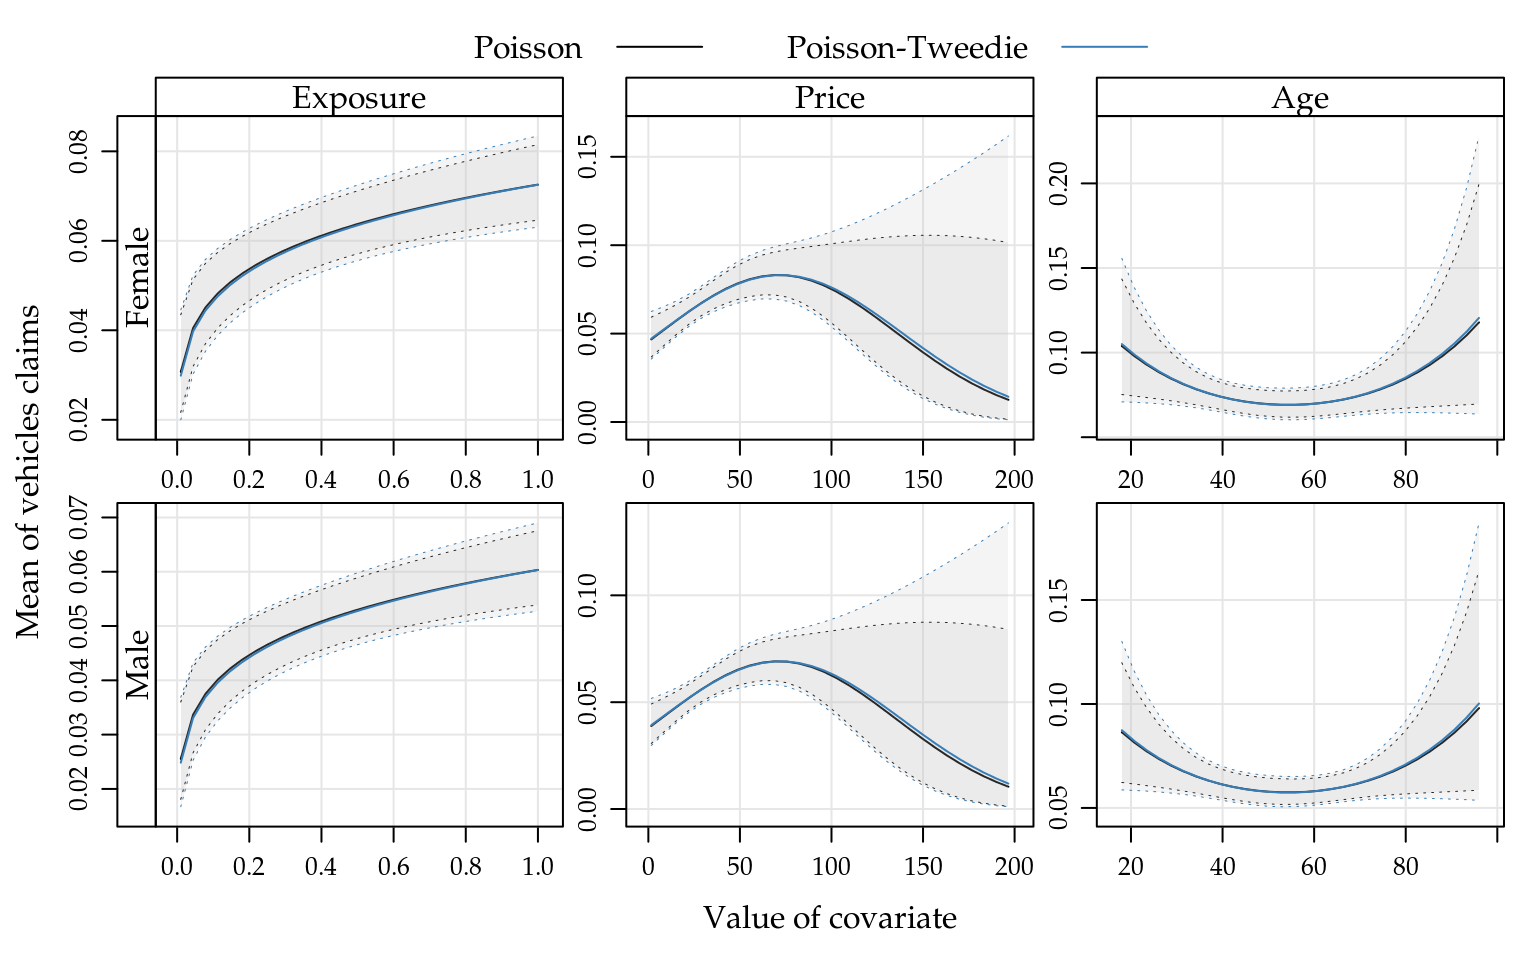
\includegraphics{rmcdbook_files/figure-latex/claims-pred-1} \end{center}

Para avaliar o poder preditivo dos modelos nós calculamos as frequências
estimadas pelos dois modelos considerados e comparamos com as
observadas. As frequências estimadas \(\hat{\mathrm{Fr}}\), para um dado
valor \(y\) são calculadas como

\[
\hat{\mathrm{Fr}}(y) = \sum_{i=1}^n \Pr(Y=y \mid \boldsymbol{\hat{\theta}}_i)
\]

Onde \(\Pr(Y=y \mid \hat{\boldsymbol{\theta}}_i)\) é a função massa de
probabilidade definida pelo conjunto de parâmetros
\(\boldsymbol{\hat{\theta}}_i\). Para o modelo Poisson
\(\hat{\boldsymbol{\theta}}_i = \hat{\mu}_i\) e para o modelo
Poisson-Tweedie
\(\hat{\boldsymbol{\theta}}_i = [\hat{\mu}_i \hat{\phi}=4.359] \hat{p}=1.832]\).
For Poisson-Tweedie model we evaluate the integral using the
Gauss-Laguerre method (with 100 points). The results shows that
Poisson-Tweedie model offers a better fit with adjust frequencies very
close of observed frequencies.

\begin{Shaded}
\begin{Highlighting}[]
\NormalTok{## Adjust frequencies by models}

\NormalTok{## Calcule probabilities}
\NormalTok{X <-}\StringTok{ }\KeywordTok{model.matrix}\NormalTok{(form1, }\DataTypeTok{data =} \NormalTok{seguros)}
\NormalTok{y <-}\StringTok{ }\DecValTok{0}\NormalTok{:}\DecValTok{6}
\NormalTok{n <-}\StringTok{ }\KeywordTok{nrow}\NormalTok{(seguros)}
\NormalTok{freqs <-}\StringTok{ }\KeywordTok{list}\NormalTok{()}

\NormalTok{## Observed}
\NormalTok{freqs$Obs <-}\StringTok{ }\KeywordTok{with}\NormalTok{(seguros, }\KeywordTok{sapply}\NormalTok{(y, function(x) \{}
    \KeywordTok{sum}\NormalTok{(nclaims ==}\StringTok{ }\NormalTok{x)}
\NormalTok{\}))}

\NormalTok{## By Poisson}
\NormalTok{muPO <-}\StringTok{ }\KeywordTok{exp}\NormalTok{(X %*%}\StringTok{ }\KeywordTok{coef}\NormalTok{(m1PO))}
\NormalTok{probsPO <-}\StringTok{ }\KeywordTok{do.call}\NormalTok{(}
    \StringTok{"rbind"}\NormalTok{,}
    \KeywordTok{lapply}\NormalTok{(muPO, function(mui) \{}
        \NormalTok{py <-}\StringTok{ }\KeywordTok{dpois}\NormalTok{(y, }\DataTypeTok{lambda =} \NormalTok{mui)}
    \NormalTok{\}))}
\NormalTok{freqs$PO <-}\StringTok{ }\KeywordTok{round}\NormalTok{(}\KeywordTok{apply}\NormalTok{(probsPO, }\DecValTok{2}\NormalTok{, sum))}

\NormalTok{## By Poisson-Tweedie}
\NormalTok{##  -- very time consuming.}
\NormalTok{muPT <-}\StringTok{ }\KeywordTok{exp}\NormalTok{(X %*%}\StringTok{ }\KeywordTok{coef}\NormalTok{(m1PT, }\DataTypeTok{type =} \StringTok{"beta"}\NormalTok{)$Estimates)}
\NormalTok{phi <-}\StringTok{ }\KeywordTok{with}\NormalTok{(}\KeywordTok{coef}\NormalTok{(m1PT), Estimates[Type ==}\StringTok{ "tau"}\NormalTok{])}
\NormalTok{power <-}\StringTok{ }\KeywordTok{with}\NormalTok{(}\KeywordTok{coef}\NormalTok{(m1PT), Estimates[Type ==}\StringTok{ "power"}\NormalTok{])}
\NormalTok{probsPT <-}\KeywordTok{do.call}\NormalTok{(}
    \StringTok{"rbind"}\NormalTok{,}
    \KeywordTok{lapply}\NormalTok{(muPT, function(mui) \{}
        \NormalTok{py <-}\StringTok{ }\KeywordTok{dptw}\NormalTok{(}\DataTypeTok{y =} \NormalTok{y, }\DataTypeTok{mu =} \NormalTok{mui, }\DataTypeTok{phi =} \NormalTok{phi,}
                   \DataTypeTok{power =} \NormalTok{power, }\DataTypeTok{n_pts =} \DecValTok{100}\NormalTok{,}
                   \DataTypeTok{method =} \StringTok{"laguerre"}\NormalTok{)}
    \NormalTok{\}))}
\NormalTok{freqs$PT <-}\StringTok{ }\KeywordTok{round}\NormalTok{(}\KeywordTok{apply}\NormalTok{(probsPT, }\DecValTok{2}\NormalTok{, sum))}
\NormalTok{tabf <-}\StringTok{ }\KeywordTok{ldply}\NormalTok{(freqs)}

\KeywordTok{colnames}\NormalTok{(tabf) <-}\StringTok{ }\KeywordTok{c}\NormalTok{(}\StringTok{""}\NormalTok{, y)}
\NormalTok{tabf}
\end{Highlighting}
\end{Shaded}

\begin{verbatim}
##           0   1   2  3 4 5 6
## 1 Obs 15689 602 166 22 3 1 0
## 2  PO 15498 953  31  1 0 0 0
## 3  PT 15673 663 121 26 6 2 0
\end{verbatim}

\section{Radiation-induced chromosome aberration
counts}\label{radiation-induced-chromosome-aberration-counts}

In biological dosimetry studies essentially the response variables are
data counts. These experiments measure the number of chromosome
aberrations in human lymphocytes after to controlled exposure of
ionizing radiation. The aim of the studies are analyse the biological
effects induced by ionizing radiation. The aberrations most commonly
mensured are the dicentrics, centric rings, and micronucle .

In this section the dataset considered was obtained after irradiating
blood samples with five different doses between 0.1 and 1 Gy of 2.1 MeV
neutrons. In this case, the frequencies of dicentrics and centric rings
after a culture of 72 hours are analysed. The dataset was analysed by
\citet{Oliveira2006}, as an example of zero-inflated data and
\citet{Bonat2016b}, using extend Poisson-Tweedie approach.

The data are available in \texttt{data/chromossome.rda} file. In
\texttt{R} it can be loaded with

\begin{Shaded}
\begin{Highlighting}[]
\NormalTok{##----------------------------------------------------------------------}
\NormalTok{## Load}
\KeywordTok{load}\NormalTok{(}\StringTok{"./data/chromosome.rda"}\NormalTok{)}
\KeywordTok{str}\NormalTok{(chromosome)}
\end{Highlighting}
\end{Shaded}

\begin{verbatim}
## 'data.frame':    5232 obs. of  2 variables:
##  $ ndic: num  0 0 0 0 0 0 0 0 0 0 ...
##  $ dose: num  0.1 0.1 0.1 0.1 0.1 0.1 0.1 0.1 0.1 0.1 ...
\end{verbatim}

The Figure \ref{fig:desc-chromo} shows the frequencies chromosome
aberrations (left) and average of chromosome aberrations by radiation
doses (right). Note that the highest frequencies are observed for zero
counts and the averages are between 0 and 1, suggesting excess zero.

\begin{figure}[h]

{\centering 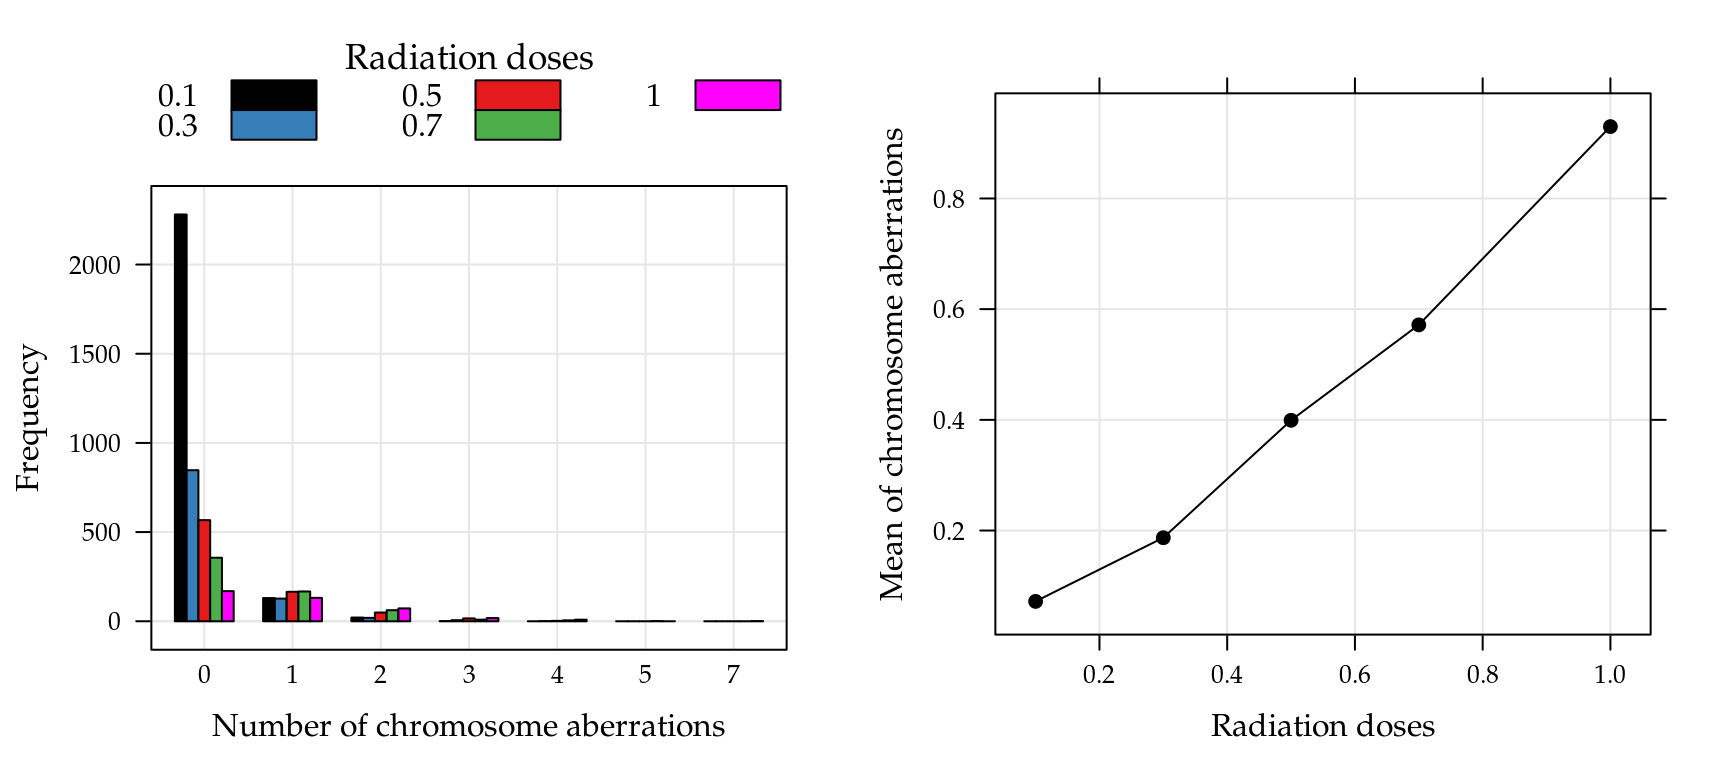
\includegraphics{rmcdbook_files/figure-latex/desc-chromo-1} 

}

\caption{Observed frequencies of the chromosome aberrations counts by radiation doses (left) and means of chromosome aberrations for each radiation doses (right).}\label{fig:desc-chromo}
\end{figure}

For this application we fit the Poisson, Gamma-Count, COM-Poisson and
Poisson-Tweedie distributions. The linear predictor considered is a
quadratic dose model, follow \citet{Bonat2016b}. The codes below fit the
four models using the \texttt{MRDCd} and \texttt{mcglm} packages. Note
that for \texttt{MRDCr::cmp} function we need specify \texttt{sumto},
the number of increments for a infinite sum, i.e in this case
\(Z(\hat{\lambda}_i, \hat{\nu}) = \sum_j^{50}\hat{\lambda}_i^j / (j!)^{\hat{\nu}}\).

\begin{Shaded}
\begin{Highlighting}[]
\NormalTok{##----------------------------------------------------------------------}
\NormalTok{## Modelling}
\NormalTok{form <-}\StringTok{ }\NormalTok{ndic ~}\StringTok{ }\NormalTok{dose +}\StringTok{ }\KeywordTok{I}\NormalTok{(dose^}\DecValTok{2}\NormalTok{)}

\NormalTok{m0PO <-}\StringTok{ }\KeywordTok{glm}\NormalTok{(form, }\DataTypeTok{family =} \NormalTok{poisson, }\DataTypeTok{data =} \NormalTok{chromosome)}
\NormalTok{m0GC <-}\StringTok{ }\KeywordTok{gcnt}\NormalTok{(form, }\DataTypeTok{data =} \NormalTok{chromosome)}
\NormalTok{m0CP <-}\StringTok{ }\KeywordTok{cmp}\NormalTok{(form, }\DataTypeTok{data =} \NormalTok{chromosome, }\DataTypeTok{sumto =} \DecValTok{50}\NormalTok{)}
\NormalTok{m0PT <-}\StringTok{ }\KeywordTok{mcglm}\NormalTok{(}
    \DataTypeTok{linear_pred =} \KeywordTok{c}\NormalTok{(form),}
    \DataTypeTok{matrix_pred =} \KeywordTok{list}\NormalTok{(}\KeywordTok{mc_id}\NormalTok{(chromosome)),}
    \DataTypeTok{link =} \StringTok{"log"}\NormalTok{,}
    \DataTypeTok{variance =} \StringTok{"poisson_tweedie"}\NormalTok{,}
    \DataTypeTok{power_fixed =} \OtherTok{FALSE}\NormalTok{,}
    \DataTypeTok{data =} \NormalTok{chromosome)}
\end{Highlighting}
\end{Shaded}

\begin{verbatim}
## Automatic initial values selected.
\end{verbatim}

No issues were reported during the estimation process. A better research
about the algorithm covergence for Poisson-Tweedie models is implemented
by \texttt{mcglm::plot(model,\ type\ =\ "algorithm")}. This four graphs
shows the trajectory or iterations of the fitting algorithm, we can see
that both cases the lines converged.

\begin{Shaded}
\begin{Highlighting}[]
\NormalTok{## Check algorithm convergence}
\KeywordTok{plot}\NormalTok{(m0PT, }\DataTypeTok{type =} \StringTok{"algorithm"}\NormalTok{)}
\end{Highlighting}
\end{Shaded}

\begin{center}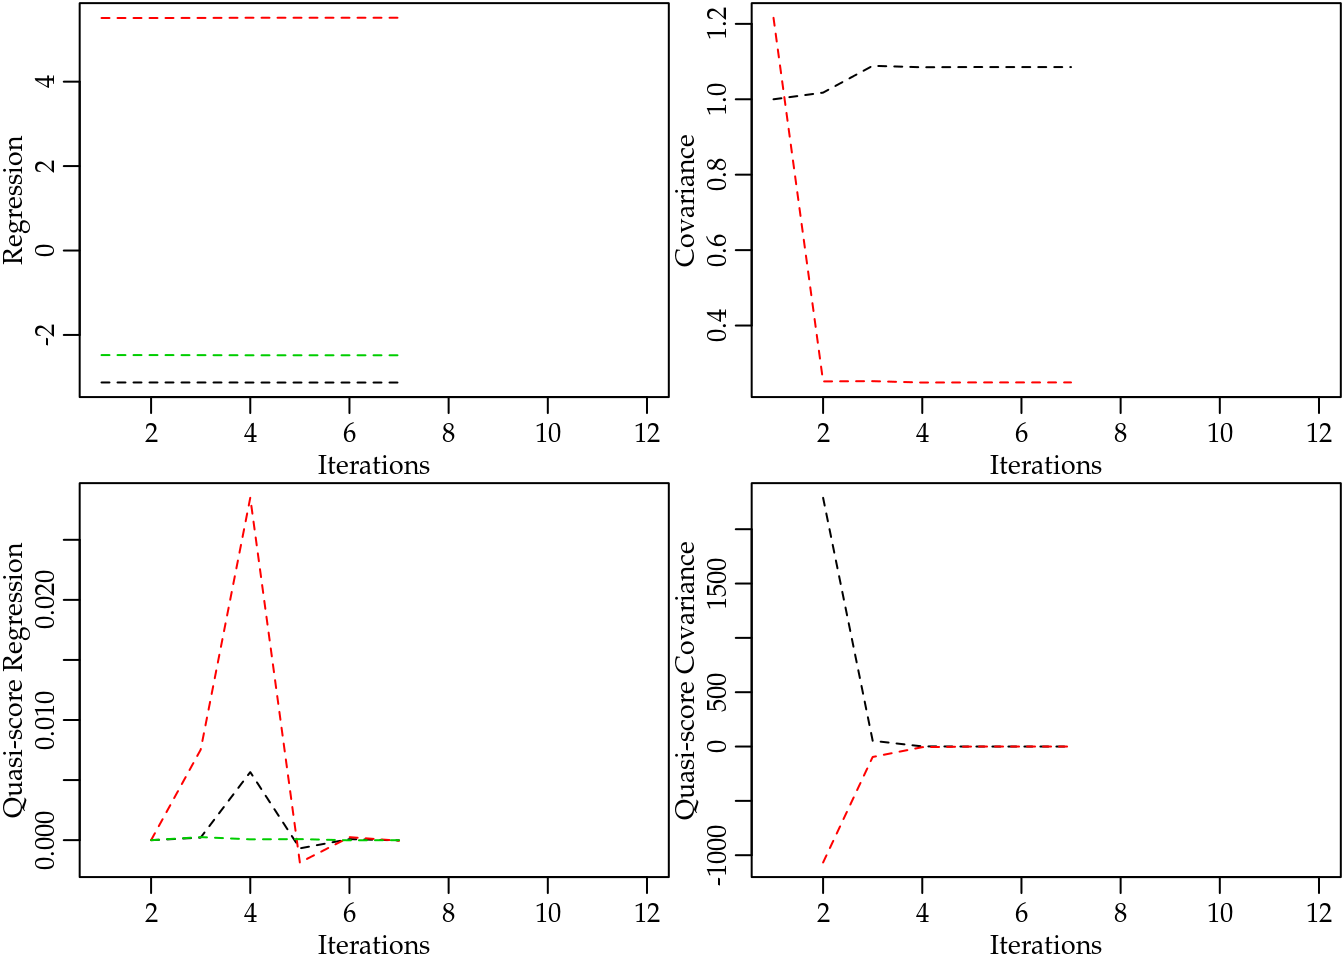
\includegraphics{rmcdbook_files/figure-latex/conv-chromo-1} \end{center}

For the COM-Poisson and Gamma-Count we can see the \texttt{details}
slots, (\texttt{model@details}). This shows the components list of
\texttt{optim}, the list object \texttt{convergence} when 0 means that
optimization was successful and \texttt{counts} shows the number of
calls to log-likelihood function and numerical gradient function. Note
the in this case the COM-Poisson model required fewer interactions than
Gamma-Count model. However, we don't evaluate the time of fit because to
compute log-likelihood function for COM-Poisson is more difficult than
for Gamma-Count.

\begin{Shaded}
\begin{Highlighting}[]
\NormalTok{## Check optim convergence}
\KeywordTok{do.call}\NormalTok{(}\StringTok{"rbind"}\NormalTok{,}
        \KeywordTok{lapply}\NormalTok{(}\KeywordTok{list}\NormalTok{(}\StringTok{"GC"} \NormalTok{=}\StringTok{ }\NormalTok{m0GC, }\StringTok{"CP"} \NormalTok{=}\StringTok{ }\NormalTok{m0CP),}
               \NormalTok{function(model) \{}
                   \KeywordTok{c}\NormalTok{(model@details$counts,}
                     \StringTok{"convergence"} \NormalTok{=}\StringTok{ }\NormalTok{model@details$convergence)}
               \NormalTok{\}))}
\end{Highlighting}
\end{Shaded}

\begin{verbatim}
##    function gradient convergence
## GC       46       16           0
## CP       29       10           0
\end{verbatim}

For COM-POisson model, we also need verify that the number of increments
for \(Z(\hat{\lambda}_i, \hat{\nu})\) is satisfactory for accurate sums.
The function \texttt{MRDCr::covergencez} shows a number of increments
necessary for a given tolerance. For each line represent the \(i\)th
observation, as we only have five different doses only five lines are
showed. Note that the \texttt{sumto=50} is more than necessary for the
convergence of all constansts.

\begin{Shaded}
\begin{Highlighting}[]
\NormalTok{## Check Z(lambda, nu) convergence}
\KeywordTok{convergencez}\NormalTok{(m0CP, }\DataTypeTok{tol =} \FloatTok{1e-5}\NormalTok{)}
\end{Highlighting}
\end{Shaded}

\begin{center}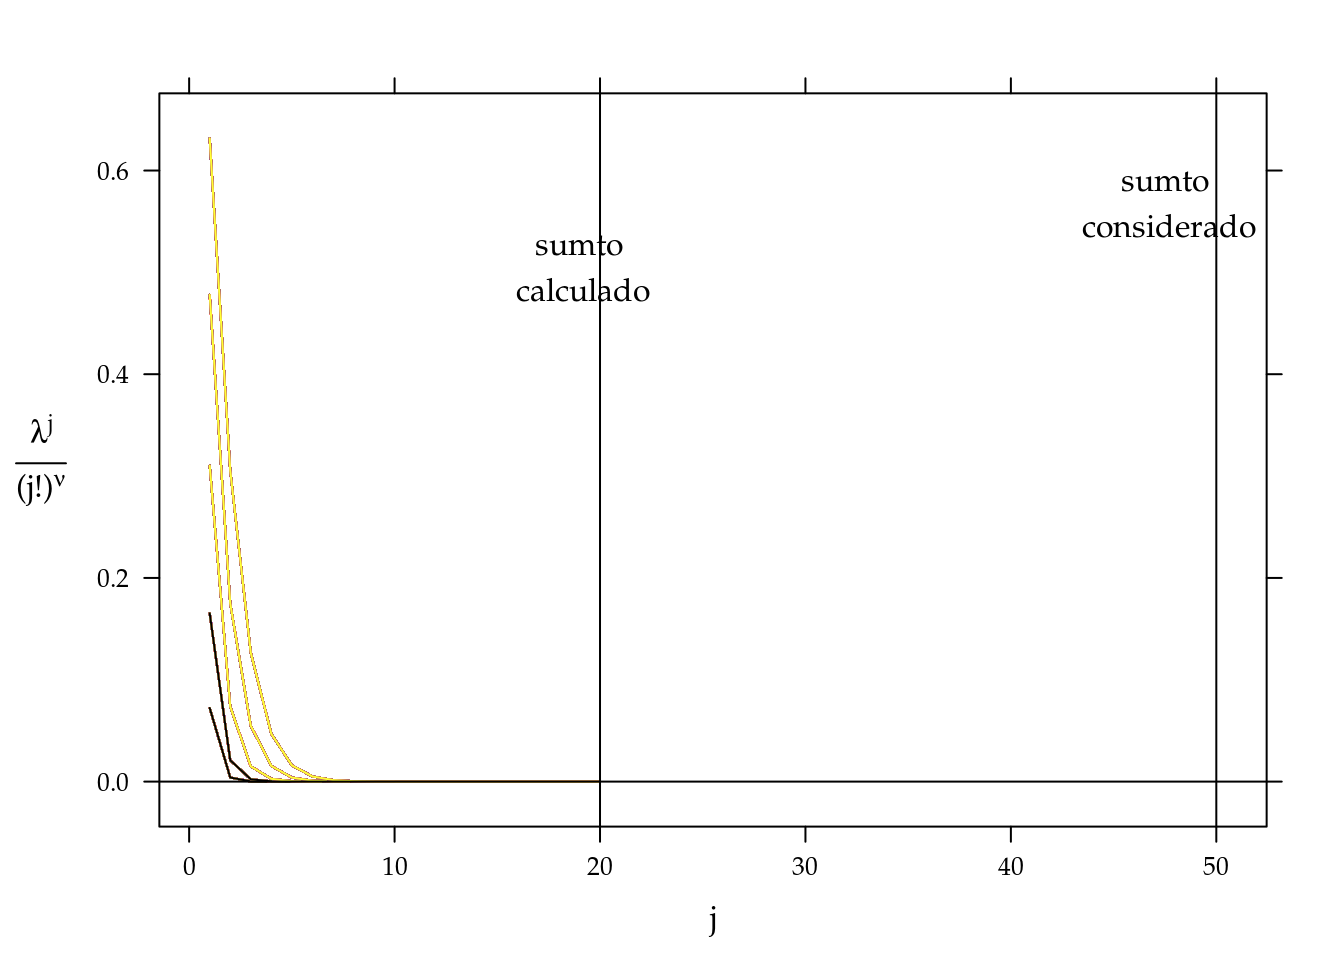
\includegraphics{rmcdbook_files/figure-latex/unnamed-chunk-58-1} \end{center}

For compare models we used the log-likelihood value and AIC and BIC
criteria. In the Gamma-Count and COM-Poisson the measures are easily
obtained by \texttt{logLik}, \texttt{AIC} and \texttt{BIC} functions. In
the Poisson-Tweedie model this functions are not implemented, because
the models are estimated only by second-moments assumptions. However, in
this case we can compute log-likelihood, and consequently AIC and BIC
criteria. This is possible beacause the parameter \(p\) was estimated on
1.085. The codes below compute these measures for the four models. Note
that in R we only implement \texttt{logLik.mcglm} function, the other
functions \texttt{AIC} and \texttt{BIC} are methods for \texttt{logLik}
objects.

The measures of goodness-of-fit show that Poisson-Tweedie approach is
more suitable in this case. Gamma-Count and COM-Poisson models present
similar results and Poisson model the worse results. This is attributed
to the inadequate assumption of equidespersion and excess of zeros.

\begin{Shaded}
\begin{Highlighting}[]
\NormalTok{##----------------------------------------------------------------------}
\NormalTok{## Goodness of fit}

\NormalTok{## Compute logLik for Poisson-Tweedie}
\NormalTok{##    ** especific for this example}
\NormalTok{logLik.mcglm <-}\StringTok{ }\NormalTok{function(object) \{}
    \NormalTok{y <-}\StringTok{ }\KeywordTok{c}\NormalTok{(}\DecValTok{0}\NormalTok{:}\DecValTok{5}\NormalTok{, }\DecValTok{7}\NormalTok{)}
    \NormalTok{data <-}\StringTok{ }\KeywordTok{data.frame}\NormalTok{(}\DataTypeTok{dose =} \KeywordTok{unique}\NormalTok{(chromosome$dose))}
    \NormalTok{## ---}
    \NormalTok{form <-}\StringTok{ }\KeywordTok{update}\NormalTok{(object$linear_pred[[}\DecValTok{1}\NormalTok{]], }\OtherTok{NULL} \NormalTok{~}\StringTok{ }\NormalTok{.)}
    \NormalTok{X <-}\StringTok{ }\KeywordTok{model.matrix}\NormalTok{(form, data)}
    \NormalTok{mu <-}\StringTok{ }\KeywordTok{exp}\NormalTok{(X %*%}\StringTok{ }\KeywordTok{coef}\NormalTok{(object, }\DataTypeTok{type =} \StringTok{"beta"}\NormalTok{)$Estimates)}
    \NormalTok{phi <-}\StringTok{ }\KeywordTok{with}\NormalTok{(}\KeywordTok{coef}\NormalTok{(object), Estimates[Type ==}\StringTok{ "tau"}\NormalTok{])}
    \NormalTok{power <-}\StringTok{ }\KeywordTok{with}\NormalTok{(}\KeywordTok{coef}\NormalTok{(object), Estimates[Type ==}\StringTok{ "power"}\NormalTok{])}
    \NormalTok{obs <-}\StringTok{ }\KeywordTok{xtabs}\NormalTok{(~ndic +}\StringTok{ }\NormalTok{dose, }\DataTypeTok{data =} \NormalTok{chromosome)}
    \NormalTok{matpred <-}\StringTok{ }\KeywordTok{do.call}\NormalTok{(}\StringTok{"cbind"}\NormalTok{, }\KeywordTok{lapply}\NormalTok{(mu, function(mui) \{}
        \KeywordTok{dptw}\NormalTok{(}\DataTypeTok{y =} \NormalTok{y, }\DataTypeTok{mu =} \NormalTok{mui, }\DataTypeTok{phi =} \NormalTok{phi, }\DataTypeTok{power =} \NormalTok{power,}
             \DataTypeTok{n_pts =} \DecValTok{180}\NormalTok{, }\StringTok{"laguerre"}\NormalTok{)}
    \NormalTok{\}))}
    \NormalTok{ll <-}\StringTok{ }\KeywordTok{sum}\NormalTok{(}\KeywordTok{log}\NormalTok{(matpred) *}\StringTok{ }\NormalTok{obs)}
    \KeywordTok{attr}\NormalTok{(ll, }\StringTok{"df"}\NormalTok{) <-}\StringTok{ }\KeywordTok{nrow}\NormalTok{(}\KeywordTok{coef}\NormalTok{(object))}
    \KeywordTok{attr}\NormalTok{(ll, }\StringTok{"nobs"}\NormalTok{) <-}\StringTok{ }\NormalTok{m0PT$n_obs}
    \KeywordTok{class}\NormalTok{(ll) <-}\StringTok{ "logLik"}
    \KeywordTok{return}\NormalTok{(ll)}
\NormalTok{\}}

\NormalTok{## Compute table of gof}
\NormalTok{models <-}\StringTok{ }\KeywordTok{list}\NormalTok{(}\StringTok{"Poisson"} \NormalTok{=}\StringTok{ }\NormalTok{m0PO, }\StringTok{"Gamma-Count"} \NormalTok{=}\StringTok{ }\NormalTok{m0GC,}
               \StringTok{"COM-Poisson"} \NormalTok{=}\StringTok{ }\NormalTok{m0CP, }\StringTok{"Poisson-Tweedie"} \NormalTok{=}\StringTok{ }\NormalTok{m0PT)}
\NormalTok{(measures <-}\StringTok{ }\KeywordTok{sapply}\NormalTok{(models, function(x)}
    \KeywordTok{c}\NormalTok{(}\StringTok{"LogLik"} \NormalTok{=}\StringTok{ }\KeywordTok{logLik}\NormalTok{(x), }\StringTok{"AIC"} \NormalTok{=}\StringTok{ }\KeywordTok{AIC}\NormalTok{(x), }\StringTok{"BIC"} \NormalTok{=}\StringTok{ }\KeywordTok{BIC}\NormalTok{(x))))}
\end{Highlighting}
\end{Shaded}

\begin{verbatim}
##        Poisson Gamma-Count COM-Poisson Poisson-Tweedie
## LogLik   -2995       -2966       -2967           -2951
## AIC       5997        5940        5943            5911
## BIC       6016        5966        5969            5944
\end{verbatim}

The parameters estimates can be obtained by \texttt{summary} methods.
The codes below shows the estimates of location and dispersion
parameters. Note that the estimates for the location parameters were
very close in Poisson, COM-Poisson and Poisson-Tweedie. For the
Gamma-Count model the estimates are many differents though the signs are
the same. Regarding the standard deviations, we have the Poisson and
COM-Poisson very close, Poisson-Tweedie with standard deviations a
little bigger and the Gamma-Count much bigger than others, totally
dissagre.

\begin{Shaded}
\begin{Highlighting}[]
\NormalTok{##----------------------------------------------------------------------}
\NormalTok{## Parameter estimates}
\NormalTok{par <-}\StringTok{ }\KeywordTok{list}\NormalTok{()}
\NormalTok{par$PO <-}\StringTok{ }\KeywordTok{rbind}\NormalTok{(}\OtherTok{NA}\NormalTok{, }\KeywordTok{summary}\NormalTok{(m0PO)$coefficients[, }\DecValTok{1}\NormalTok{:}\DecValTok{2}\NormalTok{])}
\NormalTok{par$GC <-}\StringTok{ }\KeywordTok{summary}\NormalTok{(m0GC)@coef[, }\DecValTok{1}\NormalTok{:}\DecValTok{2}\NormalTok{]}
\NormalTok{par$CP <-}\StringTok{ }\KeywordTok{summary}\NormalTok{(m0CP)@coef[, }\DecValTok{1}\NormalTok{:}\DecValTok{2}\NormalTok{]}
\NormalTok{par$PT <-}\StringTok{ }\KeywordTok{rbind}\NormalTok{(}\KeywordTok{summary}\NormalTok{(m0PT)[[}\DecValTok{1}\NormalTok{]]$tau[, }\DecValTok{1}\NormalTok{:}\DecValTok{2}\NormalTok{],}
               \KeywordTok{summary}\NormalTok{(m0PT)[[}\DecValTok{1}\NormalTok{]]$Regression[, }\DecValTok{1}\NormalTok{:}\DecValTok{2}\NormalTok{])}
\end{Highlighting}
\end{Shaded}

\begin{verbatim}
## Call: ndic ~ dose + I(dose^2)
## 
## Link function: log
## Variance function: poisson_tweedie
## Covariance function: identity
## Regression:
##             Estimates Std.error Z value
## (Intercept)     -3.13     0.106  -29.40
## dose             5.51     0.408   13.52
## I(dose^2)       -2.48     0.342   -7.26
## 
## Power:
##   Estimates Std.error Z value
## 1      1.09       0.3    3.62
## 
## Dispersion:
##   Estimates Std.error Z value
## 1     0.249       0.1    2.48
## 
## Algorithm: chaser
## Correction: TRUE
## Number iterations: 7Call: ndic ~ dose + I(dose^2)
## 
## Link function: log
## Variance function: poisson_tweedie
## Covariance function: identity
## Regression:
##             Estimates Std.error Z value
## (Intercept)     -3.13     0.106  -29.40
## dose             5.51     0.408   13.52
## I(dose^2)       -2.48     0.342   -7.26
## 
## Power:
##   Estimates Std.error Z value
## 1      1.09       0.3    3.62
## 
## Dispersion:
##   Estimates Std.error Z value
## 1     0.249       0.1    2.48
## 
## Algorithm: chaser
## Correction: TRUE
## Number iterations: 7
\end{verbatim}

\begin{Shaded}
\begin{Highlighting}[]
\KeywordTok{do.call}\NormalTok{(}\StringTok{"cbind"}\NormalTok{, par)}
\end{Highlighting}
\end{Shaded}

\begin{verbatim}
##             PO.Estimate PO.Std. Error GC.Estimate GC.Std. Error
##                      NA            NA      -0.749         0.134
## (Intercept)       -3.12        0.0968      -6.091         0.798
## dose               5.51        0.3693      10.468         1.472
## I(dose^2)         -2.48        0.3086      -5.053         0.883
##             CP.Estimate CP.Std. Error PT.Estimates PT.Std.error
##                  -0.955        0.1952        0.249        0.100
## (Intercept)      -3.114        0.0931       -3.126        0.106
## dose              5.121        0.3486        5.514        0.408
## I(dose^2)        -2.466        0.2818       -2.481        0.342
\end{verbatim}

The predict values with confidence intervals are calculated with matrix
operations, using delta method for confidence intervals. The results for
all models are presents in Figure \ref{fig:pred-chromo} together with
the observed values (black points). Though the estimates parameters are
very different the other models, for Gamma-Count the pontual prediction
is consistent with others. However, the confidence intervals for
Gamma-Count are much more conservative.

The practical interpretation of the results in \ref{fig:pred-chromo} is
that the chromosome aberration in blood samples increase as doses.
However the increase does not have the same intensity for all doses.

\begin{Shaded}
\begin{Highlighting}[]
\NormalTok{cap <-}\StringTok{ }\KeywordTok{paste}\NormalTok{(}\StringTok{"Dispersion diagram of observed chromossome aberrations and"}\NormalTok{,}
             \StringTok{"curves of predict values an confidence intervals (95}\CharTok{\textbackslash{}\textbackslash{}}\StringTok{%)"}\NormalTok{,}
             \StringTok{"based on Poisson, Gamma-Count, COM-Poisson and"}\NormalTok{,}
             \StringTok{"Poisson-Tweedie regression models."}\NormalTok{)}

\NormalTok{##-------------------------------------------}
\NormalTok{## Visualize means}

\NormalTok{## pred2 <- subset(preds, model %in% c("PO", "PT"))}
\KeywordTok{xyplot}\NormalTok{(fit ~}\StringTok{ }\NormalTok{dose,}
       \DataTypeTok{data =} \NormalTok{preds,}
       \DataTypeTok{groups =} \NormalTok{model,}
       \DataTypeTok{type =} \KeywordTok{c}\NormalTok{(}\StringTok{"g"}\NormalTok{, }\StringTok{"l"}\NormalTok{),}
       \DataTypeTok{ly =} \NormalTok{preds$lwr, }\DataTypeTok{uy =} \NormalTok{preds$upr,}
       \DataTypeTok{layout =} \KeywordTok{c}\NormalTok{(}\OtherTok{NA}\NormalTok{, }\DecValTok{1}\NormalTok{),}
       \DataTypeTok{as.table =} \OtherTok{TRUE}\NormalTok{,}
       \DataTypeTok{alpha =} \FloatTok{0.2}\NormalTok{,}
       \DataTypeTok{xlab =} \StringTok{"Radiation doses"}\NormalTok{,}
       \DataTypeTok{ylab =} \StringTok{"Mean of chromosomic aberrations"}\NormalTok{,}
       \DataTypeTok{auto.key =} \KeywordTok{list}\NormalTok{(}
           \DataTypeTok{columns =} \DecValTok{2}\NormalTok{,}
           \DataTypeTok{lines =} \OtherTok{TRUE}\NormalTok{,}
           \DataTypeTok{points =} \OtherTok{FALSE}\NormalTok{,}
           \DataTypeTok{text =} \KeywordTok{c}\NormalTok{(}\StringTok{"Poisson"}\NormalTok{, }\StringTok{"Gamma-Count"}\NormalTok{,}
                    \StringTok{"COM-Poisson"}\NormalTok{, }\StringTok{"Poisson-Tweedie"}\NormalTok{)}
       \NormalTok{),}
       \DataTypeTok{cty =} \StringTok{"bands"}\NormalTok{, }\DataTypeTok{fill =} \StringTok{"gray80"}\NormalTok{,}
       \DataTypeTok{panel =} \NormalTok{panel.superpose,}
       \DataTypeTok{panel.groups =} \NormalTok{panel.cbH,}
       \DataTypeTok{prepanel =} \NormalTok{prepanel.cbH) +}
\StringTok{    }\KeywordTok{as.layer}\NormalTok{(}
        \KeywordTok{update}\NormalTok{(xy2, }\DataTypeTok{type =} \StringTok{"p"}\NormalTok{)}
    \NormalTok{)}
\end{Highlighting}
\end{Shaded}

\begin{figure}[h]

{\centering 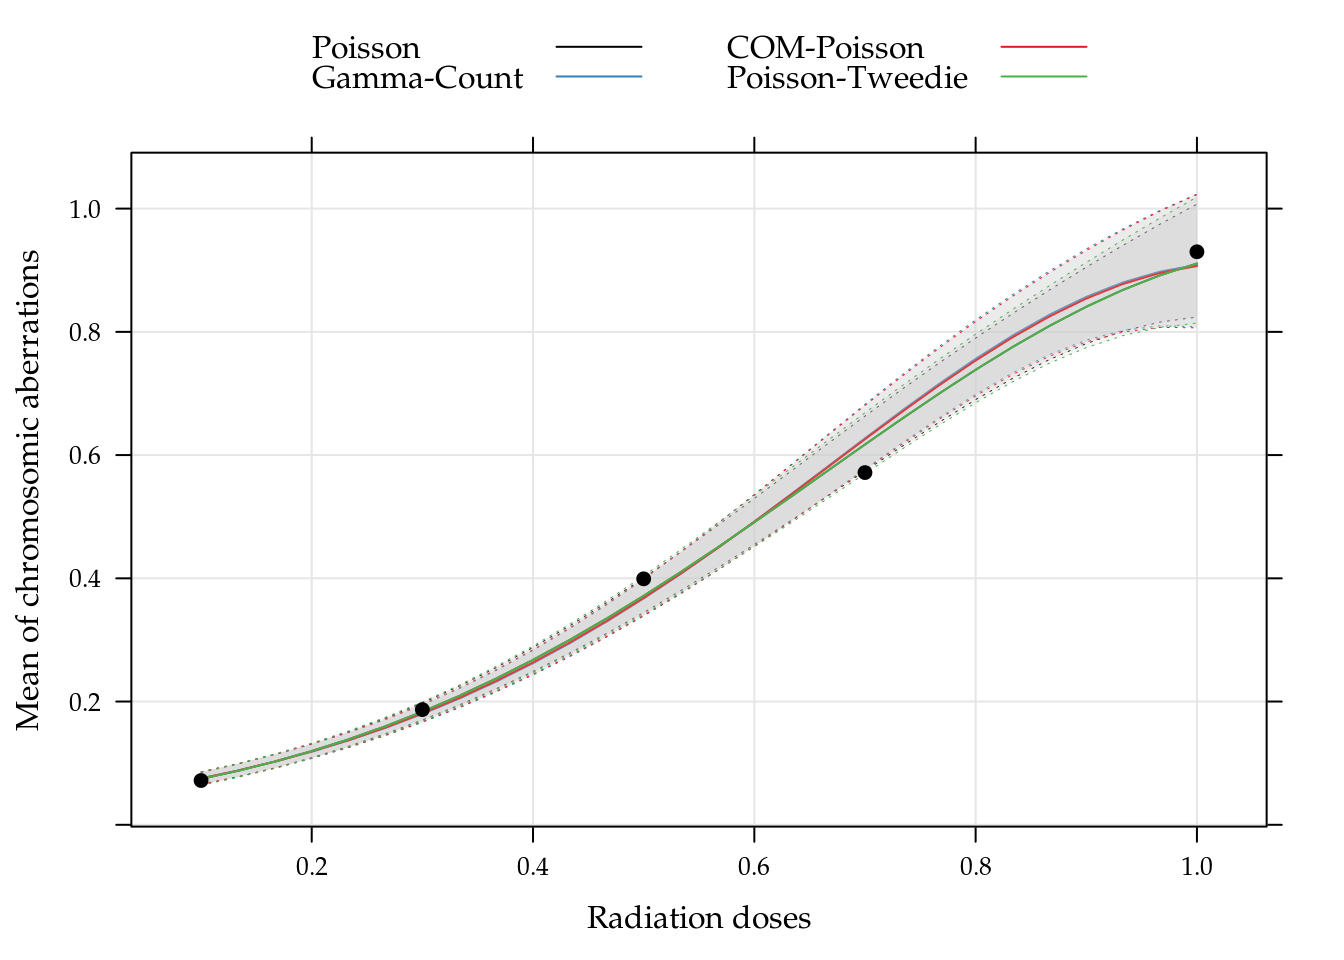
\includegraphics{rmcdbook_files/figure-latex/mean-chromo-1} 

}

\caption{Dispersion diagram of observed chromossome aberrations and curves of predict values an confidence intervals (95\%) based on Poisson, Gamma-Count, COM-Poisson and Poisson-Tweedie regression models.}\label{fig:mean-chromo}
\end{figure}

To complement the study we compute the probability distribution for the
five doses used in the experiment. This distributions are presents in
Figure \ref{fig:probs-chromo}. Note that for 0.1Gy of 2.1MeV dose
neutrons the probabilities are strongly concentrated in 0 count, for 1Gy
of 2.1MeV dose the distributions still strongly assymmetric on the
right, but the probabilities are more dispersed. It is worth mentioning
that all distribuitions, thought different, are the same average.

\begin{Shaded}
\begin{Highlighting}[]
\NormalTok{##-------------------------------------------}
\NormalTok{## Calcule probabilities}
\NormalTok{index <-}\StringTok{ }\NormalTok{preds$dose %in%}\StringTok{ }\KeywordTok{unique}\NormalTok{(chromosome$dose)}
\NormalTok{means <-}\StringTok{ }\NormalTok{preds[index, }\KeywordTok{c}\NormalTok{(}\StringTok{"model"}\NormalTok{, }\StringTok{"dose"}\NormalTok{, }\StringTok{"fit"}\NormalTok{)]}
\NormalTok{probs <-}\StringTok{ }\KeywordTok{list}\NormalTok{()}
\NormalTok{y <-}\StringTok{ }\DecValTok{0}\NormalTok{:}\DecValTok{5}

\NormalTok{## Poisson model}
\NormalTok{indPO <-}\StringTok{ }\KeywordTok{grep}\NormalTok{(}\StringTok{"PO"}\NormalTok{, means$model)}
\NormalTok{probs$PO <-}\StringTok{ }\KeywordTok{do.call}\NormalTok{(}
    \StringTok{"rbind"}\NormalTok{,}
    \KeywordTok{lapply}\NormalTok{(indPO, function(i) \{}
        \KeywordTok{with}\NormalTok{(means, \{}
            \NormalTok{py <-}\StringTok{ }\KeywordTok{dpois}\NormalTok{(y, fit[i])}
            \KeywordTok{data.frame}\NormalTok{(}\DataTypeTok{dose =} \NormalTok{dose[i], }\DataTypeTok{y =} \NormalTok{y, }\DataTypeTok{prob =} \NormalTok{py)}
        \NormalTok{\})}
    \NormalTok{\})}
\NormalTok{)}

\NormalTok{## Gamma-Count model}
\NormalTok{indGC <-}\StringTok{ }\KeywordTok{grep}\NormalTok{(}\StringTok{"GC"}\NormalTok{, means$model)}
\NormalTok{alpha <-}\StringTok{ }\KeywordTok{exp}\NormalTok{(}\KeywordTok{coef}\NormalTok{(m0GC)[}\StringTok{"alpha"}\NormalTok{])}
\NormalTok{probs$GC <-}\StringTok{ }\KeywordTok{do.call}\NormalTok{(}
    \StringTok{"rbind"}\NormalTok{,}
    \KeywordTok{lapply}\NormalTok{(indGC, function(i) \{}
        \KeywordTok{with}\NormalTok{(means, \{}
            \NormalTok{aux <-}\StringTok{ }\KeywordTok{predict}\NormalTok{(m0GC, }\DataTypeTok{newdata =} \KeywordTok{t}\NormalTok{(}\KeywordTok{cbind}\NormalTok{(X[i, ])),}
                           \DataTypeTok{type =} \StringTok{"link"}\NormalTok{)}
            \NormalTok{lambda <-}\StringTok{ }\NormalTok{alpha %*%}\StringTok{ }\KeywordTok{exp}\NormalTok{(aux)}
            \NormalTok{py <-}\StringTok{ }\KeywordTok{dgcnt}\NormalTok{(y, }\DataTypeTok{lambda =} \NormalTok{lambda, }\DataTypeTok{alpha =} \NormalTok{alpha)}
            \KeywordTok{data.frame}\NormalTok{(}\DataTypeTok{dose =} \NormalTok{dose[i], }\DataTypeTok{y =} \NormalTok{y, }\DataTypeTok{prob =} \NormalTok{py)}
        \NormalTok{\})}
    \NormalTok{\})}
\NormalTok{)}

\NormalTok{## COM-Poisson model}
\NormalTok{indCP <-}\StringTok{ }\KeywordTok{grep}\NormalTok{(}\StringTok{"CP"}\NormalTok{, means$model)}
\NormalTok{nu <-}\StringTok{ }\KeywordTok{exp}\NormalTok{(}\KeywordTok{coef}\NormalTok{(m0CP)[}\StringTok{"phi"}\NormalTok{])}
\NormalTok{sumto <-}\StringTok{ }\NormalTok{m0CP@data$sumto}
\NormalTok{probs$CP <-}\StringTok{ }\KeywordTok{do.call}\NormalTok{(}
    \StringTok{"rbind"}\NormalTok{,}
    \KeywordTok{lapply}\NormalTok{(indCP, function(i) \{}
        \KeywordTok{with}\NormalTok{(means, \{}
            \NormalTok{aux <-}\StringTok{ }\KeywordTok{predict}\NormalTok{(m0CP, }\DataTypeTok{newdata =} \KeywordTok{t}\NormalTok{(}\KeywordTok{cbind}\NormalTok{(X[i, ])),}
                           \DataTypeTok{type =} \StringTok{"link"}\NormalTok{)}
            \NormalTok{lambda <-}\StringTok{ }\KeywordTok{exp}\NormalTok{(aux)}
            \NormalTok{py <-}\StringTok{ }\KeywordTok{dcmp}\NormalTok{(y, }\DataTypeTok{lambda =} \NormalTok{lambda, }\DataTypeTok{nu =} \NormalTok{nu, }\DataTypeTok{sumto =} \NormalTok{sumto)}
            \KeywordTok{data.frame}\NormalTok{(}\DataTypeTok{dose =} \NormalTok{dose[i], }\DataTypeTok{y =} \NormalTok{y, }\DataTypeTok{prob =} \NormalTok{py)}
        \NormalTok{\})}
    \NormalTok{\})}
\NormalTok{)}

\NormalTok{## Poisson-Tweedie model}
\NormalTok{indPT <-}\StringTok{ }\KeywordTok{grep}\NormalTok{(}\StringTok{"PT"}\NormalTok{, means$model)}
\NormalTok{phi <-}\StringTok{ }\KeywordTok{with}\NormalTok{(}\KeywordTok{coef}\NormalTok{(m0PT), Estimates[Type ==}\StringTok{ "tau"}\NormalTok{])}
\NormalTok{power <-}\StringTok{ }\KeywordTok{with}\NormalTok{(}\KeywordTok{coef}\NormalTok{(m0PT), Estimates[Type ==}\StringTok{ "power"}\NormalTok{])}
\NormalTok{probs$PT <-}\StringTok{ }\KeywordTok{do.call}\NormalTok{(}
    \StringTok{"rbind"}\NormalTok{,}
    \KeywordTok{lapply}\NormalTok{(indPT, function(i) \{}
        \KeywordTok{with}\NormalTok{(means, \{}
            \NormalTok{py <-}\StringTok{ }\KeywordTok{dptw}\NormalTok{(}\DataTypeTok{y =} \NormalTok{y, }\DataTypeTok{mu =} \NormalTok{fit[i], }\DataTypeTok{phi =} \NormalTok{phi,}
                       \DataTypeTok{power =} \NormalTok{power, }\DataTypeTok{n_pts =} \DecValTok{180}\NormalTok{,}
                       \DataTypeTok{method =} \StringTok{"laguerre"}\NormalTok{)}
            \KeywordTok{data.frame}\NormalTok{(}\DataTypeTok{dose =} \NormalTok{dose[i], }\DataTypeTok{y =} \NormalTok{y, }\DataTypeTok{prob =} \NormalTok{py)}
        \NormalTok{\})}
    \NormalTok{\})}
\NormalTok{)}

\NormalTok{## Visualize the probabilities}
\NormalTok{daprobs <-}\StringTok{ }\KeywordTok{ldply}\NormalTok{(probs, }\DataTypeTok{.id =} \StringTok{"model"}\NormalTok{)}

\KeywordTok{barchart}\NormalTok{(prob ~}\StringTok{ }\NormalTok{y |}\StringTok{ }\KeywordTok{factor}\NormalTok{(dose), }\DataTypeTok{groups =} \NormalTok{model,}
         \DataTypeTok{data =} \NormalTok{daprobs,}
         \DataTypeTok{horizontal =} \OtherTok{FALSE}\NormalTok{,}
         \DataTypeTok{axis =} \NormalTok{axis.grid,}
         \DataTypeTok{as.table =} \OtherTok{TRUE}\NormalTok{,}
         \DataTypeTok{origin =} \DecValTok{0}\NormalTok{,}
         \DataTypeTok{xlab =} \StringTok{"Number of chromosomic aberrations"}\NormalTok{,}
         \DataTypeTok{ylab =} \StringTok{"Probability"}\NormalTok{,}
         \DataTypeTok{scales =} \KeywordTok{list}\NormalTok{(}\DataTypeTok{x =} \KeywordTok{list}\NormalTok{(}\DataTypeTok{labels =} \NormalTok{y)),}
         \DataTypeTok{auto.key =} \KeywordTok{list}\NormalTok{(}
             \DataTypeTok{columns =} \DecValTok{2}\NormalTok{,}
             \DataTypeTok{text =} \KeywordTok{c}\NormalTok{(}\StringTok{"Poisson"}\NormalTok{, }\StringTok{"Gamma-Count"}\NormalTok{,}
                      \StringTok{"COM-Poisson"}\NormalTok{, }\StringTok{"Poisson-Tweedie"}\NormalTok{)}
         \NormalTok{),}
         \DataTypeTok{strip =} \KeywordTok{strip.custom}\NormalTok{(}
             \DataTypeTok{strip.name =} \OtherTok{TRUE}\NormalTok{,}
             \DataTypeTok{var.name =} \StringTok{"dose"}\NormalTok{,}
             \DataTypeTok{sep =} \StringTok{" = "}
         \NormalTok{))}
\end{Highlighting}
\end{Shaded}

\begin{figure}[h]

{\centering 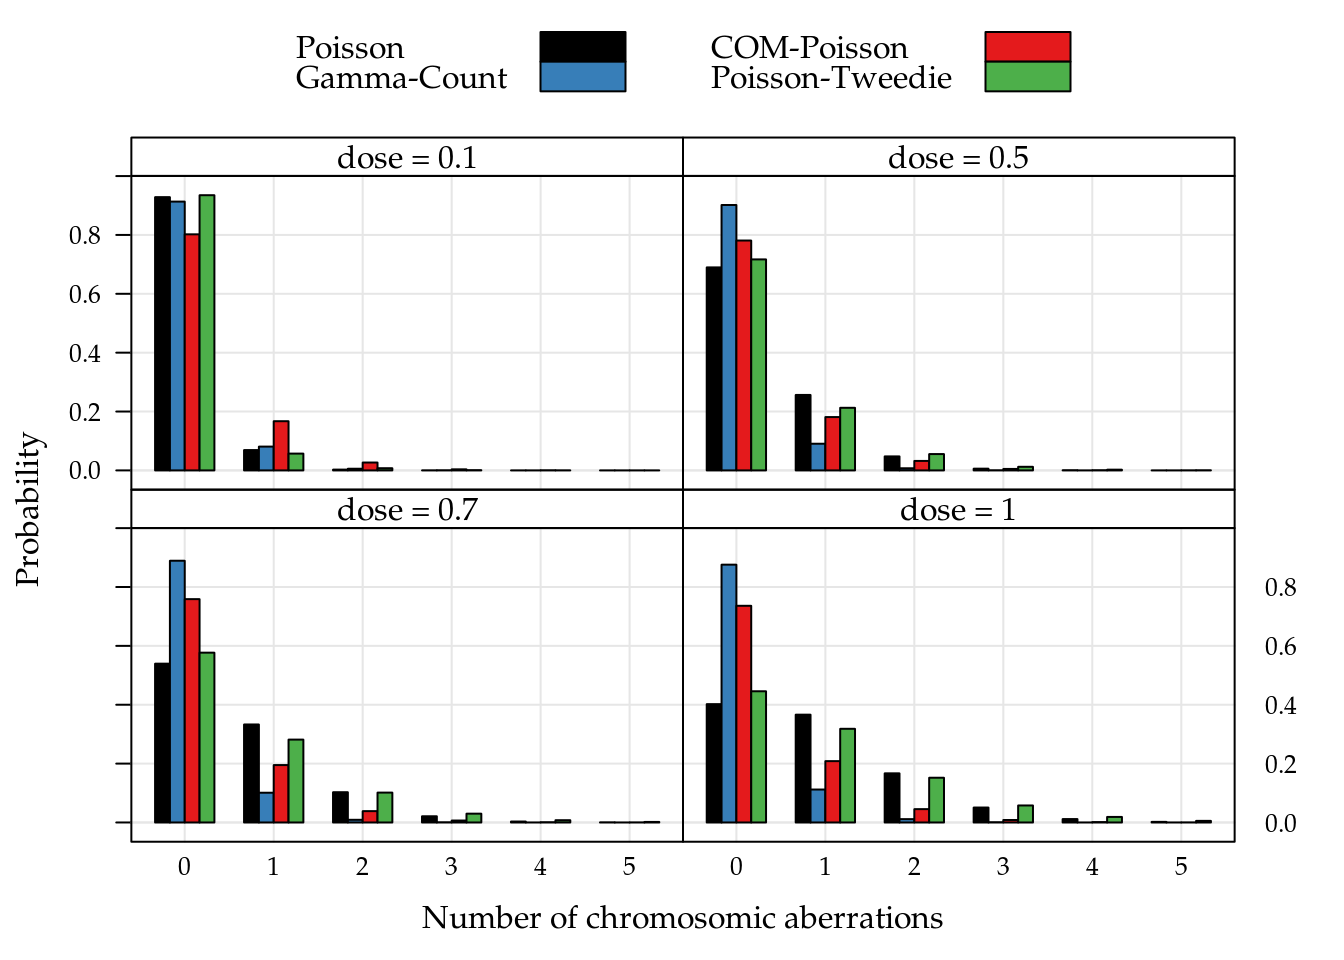
\includegraphics{rmcdbook_files/figure-latex/probs-chromo-1} 

}

\caption{Adjust probability distribution for the chromossome aberrations counts by five irradiation doses.}\label{fig:probs-chromo}
\end{figure}

\bibliography{config/rmcd.bib}


\end{document}
